\documentclass[11pt,a4paper,oneside,english]{tubaf-report}

\usepackage[english]{babel}
\usepackage{microtype}
\usepackage{amsmath,amssymb,mathtools,bm}
\usepackage{booktabs,longtable,tabularx,xltabular,array,multirow}
\usepackage{graphicx,float,caption,subcaption}
\usepackage{xcolor}
\usepackage{enumitem}
\usepackage{listings}
\usepackage{tikz}
\usetikzlibrary{arrows.meta,positioning,shapes.geometric,fit,calc,backgrounds}
\usepackage[most]{tcolorbox}
\usepackage[hidelinks]{hyperref}
\usepackage[nameinlink,noabbrev]{cleveref}

% Central report metadata.
\newcommand{\ReportTitle}{%
  Thermodynamically Consistent Neural Hyperelasticity for Multiscale
  Homogenization of Rigid-Particle-Reinforced PDMS%
}
\newcommand{\ReportSubtitle}{%
  A PyTorch--NGSolve Implementation with Periodic RVE Homogenization%
}
\newcommand{\ReportAuthor}{Vignesh Ravi}
\newcommand{\MatriculationNumber}{71807}
\newcommand{\DegreeProgramme}{Master Computational Materials Science}
\newcommand{\Semester}{Summer Semester 2026}
\newcommand{\Supervisor}{Dr.-Ing. habil. Martin Abendroth}
\newcommand{\Examiners}{%
  Prof.\ Dr.-Ing.\ habil.\ Bernhard Eidel\\
  & PD Dr.-Ing.\ habil.\ Arun Prakash\\
  & Dr.-Ing.\ Stefan Pr\"uger%
}
\newcommand{\SubmissionDate}{22 November 2026}
\newcommand{\RepositoryURL}{\url{https://github.com/Vignesh10ravi/PPP}}
\newcommand{\University}{TU Bergakademie Freiberg}


\graphicspath{{figures/}}
\setlist{nosep}
\setlength{\emergencystretch}{3em}
\setcounter{secnumdepth}{3}
\setcounter{tocdepth}{2}
\captionsetup{font=small,labelfont=bf}

\lstset{
  basicstyle=\ttfamily\small,
  frame=single,
  breaklines=true,
  columns=fullflexible,
  showstringspaces=false,
  backgroundcolor=\color{black!3}
}

% ---------- notation -------------------------------------------------------
\newcommand{\F}{\bm F}
\newcommand{\Fbar}{\overline{\bm F}}
\newcommand{\Pstress}{\bm P}
\newcommand{\Pbar}{\overline{\bm P}}
\newcommand{\Psibar}{\overline{\Psi}}
\newcommand{\Aten}{\mathbb A}
\newcommand{\Abar}{\overline{\mathbb A}}
\newcommand{\Iten}{\bm I}
\newcommand{\Cten}{\bm C}
\newcommand{\Rten}{\bm R}
\newcommand{\vfrac}{v_{\mathrm f}}
\newcommand{\dd}{\,\mathrm d}
\makeatletter
\DeclareRobustCommand{\code}[1]{{\ttfamily\let\@origus\_%
  \def\_{\@origus\allowbreak}\def\slash{/\allowbreak}#1}}
\makeatother
\newcommand{\ReportPlaceholder}[1]{%
  \textcolor{red!70!black}{\textbf{[TO COMPLETE: #1]}}%
}

% ---------- boxes ----------------------------------------------------------
\definecolor{tubafblue}{HTML}{0069B4}
\newtcolorbox{keybox}[1][]{colback=tubafblue!5,colframe=tubafblue!70,
  boxrule=0.6pt,arc=1pt,left=6pt,right=6pt,top=4pt,bottom=4pt,
  fonttitle=\bfseries\small,title={#1}}
\newtcolorbox{intuition}{colback=black!3,colframe=black!25,boxrule=0.4pt,arc=1pt,
  left=6pt,right=6pt,top=3pt,bottom=3pt,fontupper=\small}

% ---------- test-case layout (PPP guideline, Ch. 5, item 10) ---------------
\newcommand{\testcase}[2]{\subsubsection*{Test Case #1: #2}\addcontentsline{toc}{subsubsection}{Test Case #1: #2}}
\newcommand{\taim}{\par\noindent\textbf{Aim.}~}
\newcommand{\tsetup}{\par\noindent\textbf{Setup.}~}
\newcommand{\trun}{\par\noindent\textbf{How to run.}~}
\newcommand{\texpect}{\par\noindent\textbf{Expected result.}~}
\newcommand{\tobtain}{\par\noindent\textbf{Obtained result.}~}
\newcommand{\tinfer}{\par\noindent\textbf{Inference.}~}

\title[Neural Hyperelasticity for Multiscale Homogenization]{\ReportTitle}
\subtitle{\ReportSubtitle}
\subject{Personal Programming Project Report -- \Semester}
\author{\ReportAuthor}
\date{\SubmissionDate}
\publishers{\University}
\titlefoot{%
  \begin{tabular}{@{}ll@{}}
    Degree programme: & \DegreeProgramme\\
    Matriculation number: & \MatriculationNumber\\
    Supervisor: & \Supervisor\\
    Examiners: & \Examiners
  \end{tabular}%
}

\hypersetup{pdftitle={\ReportTitle}, pdfauthor={\ReportAuthor}}

\begin{document}

\pagenumbering{roman}
\maketitle
\chapter*{Abstract}
\addcontentsline{toc}{chapter}{Abstract}

Simulating a soft polymer that carries rigid particles normally requires a
microstructural finite-element (FE) problem at every macroscopic integration
point. This Personal Programming Project implements, verifies and critically
assesses an offline alternative for polydimethylsiloxane (PDMS) reinforced by
rigid glass spheres. A periodic representative volume element (RVE) with a
near-incompressible mixed $P_2/P_1$ matrix and an \emph{exactly} rigid,
freely rotating particle is solved in NGSolve. Its work-conjugate homogenized
stress follows from the assembled particle reaction, and its consistent
$9\times9$ tangent from Schur condensation of the discrete energy Hessian. The
resulting labels train a volume-fraction-conditioned, partially input-convex
neural network (pICNN) in PyTorch, whose energy is differentiated
automatically and coupled to a total-Lagrangian NGSolve Newton solver.

All 26 verification tests pass. These include the guideline-mandated checks:
six rigid-body zero eigenvalues, the twelve hourglass modes of an under-integrated hexahedron, and
single-element tests under full deformation and under stress control. The RVE satisfies periodicity and rigidity to $10^{-16}$ and the
Hill--Mandel condition to $10^{-15}$, and its tangent shows Taylor remainder
order $2.000$. Its small-strain moduli agree with the Mori--Tanaka rigid-sphere
estimate within $1.1\%$.

The surrogate assessment is deliberately split into pressure and deviatoric
stress. The pICNN reproduces pressure to a median $0.03\%$ but deviatoric stress
only to a median $76$--$83\%$ outside expansion states, and it overestimates the small-strain shear
modulus by $46$--$70\%$. The cause is identified quantitatively: with
$\kappa/\mu=10^4$ the training loss is dominated by volumetric energy, so that
removing the entire deviatoric stress would raise the validation stress loss
by only $1.5\%$. The
frozen model replaces a $134\,$s RVE solve by a $2.3\,$ms evaluation, a median
speed-up of about $5.8\times10^4$. It runs inside a macroscopic FE solve to
$5\%$ stretch with linear elements, although this solution is shown to be
volumetrically locked, while quadratic elements reach $1\%$ on two of three meshes. The project
therefore delivers a verified multiscale software pipeline, a diagnosed
limitation of the surrogate's accuracy, and a concrete remedy: isochoric
polyconvex features with a split loss, and a mixed macroscopic formulation.

\medskip\noindent\textbf{Keywords:} computational homogenization;
hyperelasticity; input-convex neural network; representative volume element;
NGSolve; PyTorch; PDMS; verification.

\chapter*{Declaration}
\addcontentsline{toc}{chapter}{Declaration}

I hereby declare that I have written this Personal Programming Project report
independently. All scientific decisions, the interpretation of the results and
the final responsibility for code and report are my own. External software,
libraries, adapted code and literature are identified in
\cref{ch:codes} and in the source documentation. The use of AI-based tools is
declared in \cref{ch:chatbots}.

\vspace{2.5cm}
\noindent Freiberg, \SubmissionDate\hfill\rule{6cm}{0.4pt}\\
\hspace*{\fill}\ReportAuthor\ (Matr.-No.\ \MatriculationNumber)

\chapter*{List of Symbols and Abbreviations}
\addcontentsline{toc}{chapter}{List of Symbols and Abbreviations}

\begin{longtable}{@{}p{0.2\textwidth}p{0.74\textwidth}@{}}
\toprule
Symbol & Meaning\\
\midrule
\endhead
$\F,\ \Fbar$ & microscopic and macroscopic deformation gradient\\
$J=\det\F$ & volume ratio\\
$\Cten=\F^{\mathsf T}\F$ & right Cauchy--Green tensor\\
$I_1,\ I_2$ & first and second principal invariants of $\Cten$\\
$\Psi,\ \Psibar$ & microscopic and homogenized strain-energy density\\
$\Pstress,\ \Pbar$ & microscopic and homogenized first Piola--Kirchhoff stress\\
$\Aten,\ \Abar$ & microscopic and homogenized material tangent $\partial\Pstress/\partial\F$ (stored as $9\times9$)\\
$\bm\sigma,\ p,\ \bm s$ & Cauchy stress, pressure $\tfrac13\operatorname{tr}\bm\sigma$, deviator $\bm\sigma-p\Iten$\\
$\bm w$ & periodic displacement fluctuation in the RVE\\
$\Rten\in SO(3)$ & particle rotation\\
$\vfrac$ & particle volume fraction\\
$\mu,\ \kappa$ & matrix shear and bulk modulus ($\mu=1$, $\kappa=10^4$)\\
$\mu_{\mathrm{eff}},\ K_{\mathrm{eff}}$ & effective small-strain shear and bulk modulus\\
$h$ & maximum element size of the macroscopic mesh\\
$\bm X,\ \bm x=\bm\varphi(\bm X)$ & reference and current position; $\bm\varphi$ is the deformation map\\
$\Omega_0,\ \Omega$ & reference body of the macroscopic problem; RVE (unit cube)\\
$\bm u,\ \delta\bm u$ & displacement and test function\\
$\bar I_1,\ \bar I_2$ & invariants of the isochoric part: $I_1=J^{2/3}\bar I_1$, $I_2=J^{4/3}\bar I_2$\\
$\bm\varepsilon$ & small-strain tensor\\
$\Pi,\ p$ & mixed (displacement--pressure) functional; Lagrange pressure\\
$\lambda$ & Lam\'e constant of the neo-Hookean reference law ($\lambda=10$, \cref{ch:theory}); in \cref{ch:methods} also an eigenvalue ($\lambda_{\min}(\bm K)$)\\
$K_{\mathrm{MT}},\ \mu_{\mathrm{MT}},\ \eta$ & Mori--Tanaka bulk and shear modulus; auxiliary modulus in \cref{eq:mt}\\
$\bm y,\ \hat{\bm y},\ \hat c$ & invariant features $[I_1,I_2,J,-\ln J]$, their standardized values, standardized volume fraction\\
$W^{+}=\mathrm{softplus}(W)$ & non-negative network weights (the symbol $\sigma$ also denotes the softplus activation in the network equations)\\
$\bm\beta,\ \bm b_l$ & biases of the energy network; bias shifts produced by the context network\\
$\Psi_{\mathrm{raw}},\ \widehat\Psi$ & network output and its normalized value (zero energy and stress at $\F=\Iten$)\\
$\mathcal L,\ w_P,\ s_\Psi,\ s_P$ & training loss, stress weight, energy and stress scales\\
$\Psi_{\mathrm{iso}},\ \Psi_{\mathrm{vol}}$ & isochoric and volumetric energy of the proposed split\\
$\bm K,\ \bm R,\ \alpha$ & tangent stiffness matrix, residual, spectral shift of the Newton fallback\\
$\bm\theta$ & rotation increment of the particle\\
$\gamma$ & amount of simple shear\\
$\epsilon,\ \varepsilon_{\mathrm{mach}}$ & finite-difference step; machine epsilon\\
$\rho$ & Spearman rank correlation\\
\midrule
Abbreviation & Meaning\\
\midrule
AD & automatic differentiation\\
DOF & degree of freedom\\
FD & finite difference\\
MT & Mori--Tanaka\\
NH, SVK & neo-Hookean, Saint~Venant--Kirchhoff (reference material laws)\\
OCC & Open CASCADE geometry kernel used by Netgen\\
PBS & portable batch system (cluster job scheduler)\\
RMS & root mean square\\
$SO(3)$ & group of three-dimensional rotations\\
FE, FEM & finite element(s), finite-element method\\
FE$^2$ & concurrent two-scale finite-element method\\
ICNN / pICNN & (partially) input-convex neural network\\
NRMSE & normalized root-mean-square error\\
PBC & periodic boundary condition\\
PDMS & polydimethylsiloxane\\
RVE & representative volume element\\
$P_1,\ P_2$ & linear / quadratic Lagrange elements\\
\bottomrule
\end{longtable}


\tableofcontents
\clearpage
{\setlength{\parskip}{0pt}\renewcommand{\baselinestretch}{0.95}\selectfont
\listoffigures}
\listoftables
\clearpage

\pagenumbering{arabic}
\chapter{Introduction}\label{ch:intro}

\paragraph{Motivation.} Elastomers filled with stiff particles combine
the compliance of the matrix with a tunable stiffness. For PDMS with glass
beads the contrast is extreme: the matrix has a shear modulus of order
$1\,$MPa and is nearly incompressible, while glass is about five orders of
magnitude stiffer. The macroscopic response is strongly nonlinear and depends
on the particle content. A concurrent FE$^2$ simulation resolves this by
solving a microstructural boundary-value problem at every macroscopic
integration point and load step~\cite{Kouznetsova2001,Miehe2002}. Its cost scales with the product of the macroscopic and microscopic problem
sizes. The alternative pursued here is
\emph{offline} homogenization. Representative volume elements (RVEs) are solved
once for many prescribed macroscopic deformations, and a surrogate learns the
homogenized energy so that it can act as a material law in the macroscopic
solver. For a Newton solver the surrogate must return the energy $\Psibar$
together with the first Piola stress $\Pbar$ and the consistent tangent $\Abar$,
and these three quantities must be mutually consistent.

\paragraph{Objective.} The project proposal (defended in SS~2026) defined the project as a
Python implementation of a thermodynamically consistent neural material law
inside NGSolve, built in two phases:
\begin{enumerate}
  \item \emph{Phase 1 (proof of concept):} a PyTorch--NGSolve material
        bridge, trained on a neo-Hookean law and verified on elementary FE problems;
  \item \emph{Phase 2 (multiscale):} periodic PDMS--glass RVEs,
        homogenized data generation, training of a volume-fraction-conditioned
        pICNN, and its deployment in a macroscopic FE simulation.
\end{enumerate}

\paragraph{Contributions and outcome.} All software components were
implemented and verified. An exactly rigid, freely rotating particle replaced the
proposed stiffness penalty, and a Schur-condensed energy Hessian replaced the
finite-difference RVE tangent. The verification covers the guideline's mandatory
element and single-element tests. A pressure/deviatoric split of the surrogate error
reveals and explains a large shear error, and an analysis shows that the
linear-element macroscopic solution is volumetrically locked.
\Cref{tab:proposal,tab:committee} compare the proposal milestones and the
committee's recommendations with their outcome.

\paragraph{Organization.} The chapters follow the order of the PPP
guideline: theory, numerical methods, available codes, flowchart, use of AI tools,
verification, assessment, computation time, conclusion, manual, literature and
git log.

\chapter{Theory}\label{ch:theory}

\section{Finite-strain hyperelasticity}

A material point $\bm X$ of the reference body $\Omega_0$ moves to
$\bm x=\bm\varphi(\bm X)$. With the deformation gradient
$\F=\partial\bm\varphi/\partial\bm X$, $J=\det\F>0$ and $\Cten=\F^{\mathsf T}\F$,
a hyperelastic material is defined by a stored-energy density $\Psi(\F)$, from
which stress and tangent follow~\cite{Holzapfel2000}:
\begin{equation}
  P_{iJ}=\frac{\partial\Psi}{\partial F_{iJ}},\qquad
  \Aten_{iJkL}=\frac{\partial^2\Psi}{\partial F_{iJ}\,\partial F_{kL}}.
  \label{eq:PA}
\end{equation}
Because $\F$ and $\Pstress$ are not symmetric, the implementation keeps all nine
components and stores the tangent row-major as
$A^{9\times9}_{3i+J,\;3k+L}=\Aten_{iJkL}$. The proposal's $6\times6$ Voigt map
applies to symmetric strain--stress pairs and was therefore replaced. In the
total-Lagrangian setting, equilibrium is the stationarity of the potential,
\begin{equation}
  \int_{\Omega_0}\Pstress(\F):\nabla_{\!X}\delta\bm u\dd V=\delta W_{\mathrm{ext}}
  \quad\forall\,\delta\bm u,
  \label{eq:weak}
\end{equation}
and Newton's method needs $\Aten$ at exactly the same quadrature points as
$\Pstress$. The Phase~1 reference is the compressible neo-Hookean law
\begin{equation}
  \Psi_{\mathrm{NH}}=\tfrac{\mu}{2}(I_1-3)-\mu\ln J+\tfrac{\lambda}{2}(\ln J)^2,
  \qquad \mu=1,\ \lambda=10.
  \label{eq:nh}
\end{equation}

\section{Polyconvex neural energy}

A stored energy is \emph{polyconvex} if it is a convex function of
$(\F,\operatorname{cof}\F,\det\F)$. Polyconvexity implies rank-one convexity and
hence ellipticity of the tangent, and together with suitable coercivity and growth
conditions it guarantees the existence of minimizers~\cite{Ball1977}.
Following~\cite{Klein2022,Linden2023}, the network receives the feature vector
\begin{equation}
  \bm y=\bigl[\,I_1,\ I_2,\ J,\ -\ln J\,\bigr],\qquad
  I_1=\|\F\|^2,\quad I_2=\|\operatorname{cof}\F\|^2 .
\end{equation}
$I_1$ is convex in $\F$, $I_2$ is convex in $\operatorname{cof}\F$, and both $J$
and $-\ln J$ are convex in $J$. An input-convex network~\cite{Amos2017} with
non-negative weights $W^+=\mathrm{softplus}(W)$ and convex, non-decreasing
softplus activations is convex and non-decreasing in $\bm y$, so the composite
energy is polyconvex. The particle volume fraction $\vfrac$ enters only through
an unconstrained sub-network that shifts the hidden-layer biases. This makes
the network \emph{partially} input-convex: convex in the kinematic inputs for
every fixed $\vfrac$. The network uses three hidden layers of width 32 and has
5793 trainable parameters (2561 without the context sub-network, as in Phase~1). Following~\cite{Linden2023}, the raw output is normalized so that the reference
state is energy- and stress-free:
\begin{equation}
  \widehat\Psi(\F,\vfrac)=\Psi_{\mathrm{raw}}(\F,\vfrac)-\Psi_{\mathrm{raw}}(\Iten,\vfrac)
  -p_I(\vfrac)\,(J-1),\qquad
  p_I=\tfrac13\operatorname{tr}\Pstress_{\mathrm{raw}}(\Iten,\vfrac).
  \label{eq:norm}
\end{equation}
The correction depends on $\F$ only through $J$, so it is objective and affine in
a polyconvex argument. The Phase~1 network instead used the correction
$\Pstress_{\mathrm{raw}}(\Iten):(\F-\Iten)$, which is \emph{not} objective,
because $\operatorname{tr}(\Rten-\Iten)\neq0$ for a rotation $\Rten$. The
consequence is quantified in Test~V0d (\cref{sec:v0}).

\section{Periodic RVE with an exactly rigid particle}

The RVE is the unit cube $\Omega=[0,1]^3$ with a centred spherical cavity of
radius $r=(3\vfrac/4\pi)^{1/3}$, $\vfrac\in\{0.02,0.05,0.10\}$
(\cref{fig:rve}).

\begin{figure}[htbp]
\centering
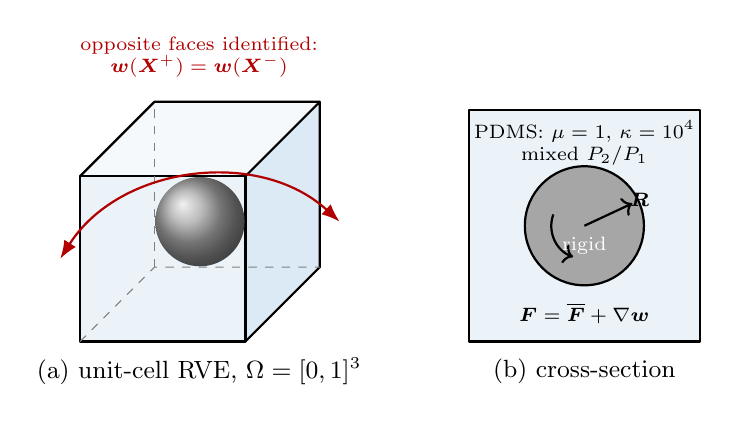
\begin{tikzpicture}[scale=2.1, line join=round]
  % (a) cube with sphere
  \begin{scope}
    \def\d{0.45}
    \fill[tubafblue!8] (0,0)--(1,0)--(1,1)--(0,1)--cycle;
    \fill[tubafblue!14] (1,0)--(1+\d,\d)--(1+\d,1+\d)--(1,1)--cycle;
    \fill[tubafblue!4] (0,1)--(1,1)--(1+\d,1+\d)--(\d,1+\d)--cycle;
    \draw[thick] (0,0)--(1,0)--(1,1)--(0,1)--cycle;
    \draw[thick] (1,0)--(1+\d,\d)--(1+\d,1+\d)--(1,1);
    \draw[thick] (0,1)--(\d,1+\d)--(1+\d,1+\d);
    \draw[dashed,black!50] (0,0)--(\d,\d)--(1+\d,\d); \draw[dashed,black!50] (\d,\d)--(\d,1+\d);
    \shade[ball color=black!35] (0.5+\d/2,0.5+\d/2) circle (0.27);
    \node[font=\small] at (0.72,-0.18) {(a) unit-cell RVE, $\Omega=[0,1]^3$};
    \draw[{Latex}-{Latex},red!70!black,thick] (-0.12,0.5) to[bend left=50] node[above,font=\scriptsize,pos=0.5]{} (1.0+\d+0.12,0.5+\d/2);
    \node[red!70!black,font=\scriptsize,align=center] at (0.72,1.72) {opposite faces identified:\\ $\bm w(\bm X^+)=\bm w(\bm X^-)$};
  \end{scope}
  % (b) cross-section
  \begin{scope}[xshift=2.35cm]
    \fill[tubafblue!8] (0,0) rectangle (1.4,1.4);
    \draw[thick] (0,0) rectangle (1.4,1.4);
    \fill[black!35] (0.7,0.7) circle (0.36);
    \draw[thick] (0.7,0.7) circle (0.36);
    \draw[->,thick] (0.7,0.7) -- ++(25:0.32) node[pos=1.15,font=\scriptsize]{$\Rten$};
    \draw[thick,->] (0.7,0.7) ++(160:0.2) arc (160:250:0.2);
    \node[font=\scriptsize,align=center] at (0.7,1.2) {PDMS: $\mu=1$, $\kappa=10^4$\\ mixed $P_2/P_1$};
    \node[font=\scriptsize,align=center,white] at (0.7,0.58) {rigid};
    \node[font=\scriptsize,align=center] at (0.7,0.17) {$\F=\Fbar+\nabla\bm w$};
    \node[font=\small] at (0.7,-0.18) {(b) cross-section};
  \end{scope}
\end{tikzpicture}
\caption[Microscale problem]{Microscale problem. (a) Periodic unit cell with one centred spherical
particle; opposite faces share their fluctuation degrees of freedom. (b) The
particle surface follows the exact rigid map \cref{eq:rigid}; the free rotation
$\Rten$ is found from moment equilibrium. Volume fractions
$\vfrac=0.02,0.05,0.10$ correspond to radii $0.168$, $0.229$ and $0.288$.
Schematic, not to scale.}
\label{fig:rve}
\end{figure}

The microscopic deformation splits into the prescribed
macroscopic part and a periodic fluctuation,
\begin{equation}
  \bm\varphi(\bm X)=\Fbar\bm X+\bm w(\bm X),\qquad
  \F=\Fbar+\nabla\bm w,\qquad \bm w(\bm X^+)=\bm w(\bm X^-),
  \label{eq:kin}
\end{equation}
so that tractions are anti-periodic in the weak sense. The near-incompressible
PDMS matrix is described by the mixed potential
\begin{equation}
  \Pi(\F,p)=\tfrac{\mu}{2}\bigl(J^{-2/3}I_1-3\bigr)+p\,(J-1)-\frac{p^2}{2\kappa},
  \qquad \mu=1,\ \kappa=10^4 ,
  \label{eq:mixed}
\end{equation}
whose stationarity in $p$ gives $p=\kappa(J-1)$. The particle is not modelled as
a stiff elastic phase. Instead, the cavity surface undergoes the exact finite
rigid motion
\begin{equation}
  \bm u_{\mathrm p}(\bm X)=(\Fbar-\Iten)\bm X_c+(\Rten-\Iten)(\bm X-\bm X_c),\qquad
  \Rten\in SO(3),
  \label{eq:rigid}
\end{equation}
where the centre $\bm X_c$ follows the macroscopic map; a common translation is a
gauge mode of the periodic problem. The rotation is free and is determined by a
vanishing resultant moment on the particle. The Hill--Mandel condition demands
equality of macroscopic and averaged microscopic power~\cite{Hill1963}; at finite
strain the work-conjugate pair is $(\Pbar,\Fbar)$~\cite{Hill1972}:
\begin{equation}
  \Pbar:\dot{\Fbar}=\frac{1}{|\Omega|}\int_{\Omega_{\mathrm m}}\Pstress:\dot{\F}\dd V
  \quad\Longrightarrow\quad
  \Pbar=\frac{1}{|\Omega|}\Bigl(\int_{\Omega_{\mathrm m}}\Pstress\dd V
  +\textstyle\sum_{iJ}(\bm r\cdot\bm b_{iJ})\,\bm e_i\otimes\bm E_J\Bigr),
  \label{eq:hm}
\end{equation}
where $\bm r$ is the assembled nodal residual of the matrix, which contains the
particle reactions, and $\bm b_{iJ}$ is the nodal lift of the particle trace
$-(\bm e_i\otimes\bm E_J)(\bm X-\bm X_c)$ produced by a unit increment of
$\bar F_{iJ}$. The second term is therefore the work of the particle reactions in
the macroscopic modes. Integrating the stress over the
deformable matrix alone would omit this work, and the result would not be
conjugate to $\Fbar$.

\section{Consistent homogenized tangent}

Let $\bm z$ collect the free fluctuation, pressure and rotation unknowns of the
discretized RVE and let $\bm H$ be the Hessian of its discrete energy with
respect to $(\Fbar,\bm z)$. Eliminating the equilibrated internal unknowns gives
the exact derivative of the homogenized stress as a Schur
complement~\cite{Miehe2002},
\begin{equation}
  \Abar=\frac{1}{|\Omega|}\Bigl(\bm H_{\bar F\bar F}-\bm H_{\bar Fz}\,
  \bm H_{zz}^{-1}\,\bm H_{z\bar F}\Bigr).
  \label{eq:schur}
\end{equation}
It is a Hessian of the relaxed energy and must therefore be major-symmetric.
Finite perturbations of $\Fbar$ serve only as verification.

\section{Small-strain reference and scale separation}\label{sec:scales}

At $\Fbar=\Iten$ the homogenized tangent of an isotropic composite reduces to an
effective bulk modulus $K_{\mathrm{eff}}$ and shear modulus $\mu_{\mathrm{eff}}$.
For rigid spheres in a matrix $(\kappa,\mu)$, the Mori--Tanaka
estimate~\cite{MoriTanaka1973}, in the form given by Benveniste~\cite{Benveniste1987},
gives
\begin{equation}
  K_{\mathrm{MT}}=\kappa+\frac{\vfrac\,(\kappa+\tfrac43\mu)}{1-\vfrac},\qquad
  \mu_{\mathrm{MT}}=\mu+\frac{\vfrac\,(\mu+\eta)}{1-\vfrac},\qquad
  \eta=\frac{\mu\,(9\kappa+8\mu)}{6(\kappa+2\mu)} .
  \label{eq:mt}
\end{equation}
For a stiffer inclusion this estimate coincides with the Hashin--Shtrikman lower
bound~\cite{HashinShtrikman1963}, and it serves as an independent check of the RVE.

Of equal importance for the following chapters is the separation of scales
inside the energy. For small strains $\bm\varepsilon$,
\begin{equation}
  \Psibar\approx\tfrac12K_{\mathrm{eff}}(\operatorname{tr}\bm\varepsilon)^2
  +\mu_{\mathrm{eff}}\,\|\operatorname{dev}\bm\varepsilon\|^2,\qquad
  K_{\mathrm{eff}}/\mu_{\mathrm{eff}}\approx(0.87\text{--}0.97)\times10^4 ,
  \label{eq:split}
\end{equation}
where the ratio follows from \cref{eq:mt} for $\vfrac=0.10$ to $0.02$.
Any measure that adds volumetric and deviatoric contributions, such as a
training loss or an error norm normalized by the total energy or stress, is
dominated by the volumetric part unless the volumetric strains are smaller than
the deviatoric ones by a factor of about $\sqrt{\mu/K}\approx10^{-2}$.
\Cref{ch:assessment} shows that this is precisely what limits the present
surrogate.

\chapter{Numerical Methods and Implementation Details}\label{ch:methods}

The implementation consists of two finite-element applications coupled through
one neural network. Offline, NGSolve solves periodic RVEs and stores energy,
stress and tangent; PyTorch trains the network on these data. Online, the trained
network is evaluated at every quadrature point of a macroscopic NGSolve model and
supplies stress and tangent to Newton's method.

\section{Choice of language and libraries}

The code is written in Python~3.11. This lets a single language host both the
finite-element library NGSolve~\cite{Schoeberl2014} (C++ core, Python front end,
symbolic differentiation of variational forms) and PyTorch~\cite{Paszke2019}
(reverse-mode automatic differentiation, optimizers). Python's overhead is
confined to orchestration. All heavy kernels run in compiled code: sparse
assembly and direct solvers in NGSolve, and batched tensor algebra in PyTorch.
NumPy handles array exchange; Matplotlib is used for plotting. All computations
use double precision.

\section{Phase 1: the PyTorch--NGSolve material bridge}\label{sec:bridge}

NGSolve has no hook for a constitutive law written in an external framework.
The bridge (\code{src\slash{}ngsolve\_umat.py}) therefore passes data through
\code{IntegrationRuleSpace} grid functions. These store one value per
quadrature point and are tied to a fixed integration rule. Each Newton
iteration performs the following steps (routine \code{assemble\_system}):
\begin{enumerate}
  \item interpolate $\F=\Iten+\nabla\bm u$ into a nine-component quadrature-point
        function and gather it as an array of shape $(n_q,3,3)$;
  \item reject non-finite values and any $J\le10^{-8}$ before calling the network;
  \item evaluate $\widehat\Psi$, $\Pstress=\partial\widehat\Psi/\partial\F$ and the nine rows of
        $\Aten=\partial\Pstress/\partial\F$ by repeated reverse-mode AD
        (\code{stress\_and\_tangent});
  \item write $\Pstress$ (9 components) and $\Aten$ (81 components, row-major
        $3i+J$) back into quadrature-point functions;
  \item assemble the residual and the consistent stiffness
        \begin{equation}
          R_a=\int_{\Omega_0}P_{iJ}\,N_{a,i,J}\dd V,\qquad
          K_{ab}=\int_{\Omega_0}N_{a,i,J}\,\Aten_{iJkL}\,N_{b,k,L}\dd V
        \end{equation}
        using \emph{the same} integration rule, and solve for the update on the
        free degrees of freedom.
\end{enumerate}
\textbf{Tricky aspects.} (i) If the residual or stiffness forms were integrated
with a rule other than the one attached to the quadrature-point space, the
material data would be evaluated at the wrong locations. NGSolve raises no error
in that case; the Newton iteration simply loses its quadratic rate. (ii) A
transposed index map or a $6\times6$ shortcut assembles the stiffness of a
different material; V3--V6 detect both. (iii) The tangent needs nine
backward passes through a graph created with \code{create\_graph=True}. This is
the dominant cost of the bridge (\cref{ch:performance}).

\section{Phase 2: periodic RVE solver}

\paragraph{Geometry and periodicity.} The cube with a spherical cavity is built
with Netgen's OCC kernel~\cite{Schoeberl1997}. Opposite faces are identified \emph{before} meshing, so
the surface meshes match node by node, and NGSolve's \code{Periodic} wrapper
shares the corresponding degrees of freedom~\cite{NGSolvePeriodic}. The unknown
is the fluctuation $\bm w$ of \cref{eq:kin}; periodicity therefore applies to $\bm w$
and not to the affine part of the displacement.

\paragraph{Mixed matrix.} The residual of \cref{eq:mixed} is discretized with
Taylor--Hood elements: $P_2$ displacement and $P_1$ pressure. This choice
satisfies the inf--sup condition~\cite{Boffi2013} and avoids the volumetric locking of a
displacement-only low-order discretization at $\kappa/\mu=10^4$~\cite{Simo1985}.
NGSolve differentiates the symbolic residual to give the exact Jacobian. The
production setting uses $h=0.22$ and integration order~10.

\paragraph{Rigid particle and free rotation.} The cavity boundary is a Dirichlet
boundary of the displacement space whose prescribed trace is the exact rigid map
\cref{eq:rigid}. The particle therefore has no deformational degrees of freedom
and no penalty parameter is needed. The three rotation coordinates are found in
an outer Newton loop (\code{src\slash{}free\_particle.py}):
\begin{enumerate}
  \item for the current $\Rten$, solve the mixed periodic RVE by Newton's method (tolerance $10^{-8}$ in production, $10^{-10}$ in the tests);
  \item assemble the resultant moment $\bm m$ of the reactions on the particle;
  \item compute the exact condensed rotational Hessian $\partial\bm m/\partial\bm\theta$
        by one sparse factorization and three sensitivity solves;
  \item update multiplicatively, $\Rten\leftarrow\exp([\delta\bm\theta]_\times)\Rten$
        (Rodrigues' formula), until the moment residual is below $10^{-9}$.
\end{enumerate}
Large or strongly compressive loads start from the identity and are approached
by adaptive load continuation with previous-state or secant predictors.

\paragraph{Homogenization and tangent.} The homogenized energy is the
equilibrated potential divided by $|\Omega|$. The stress is evaluated with
\cref{eq:hm}, adding the matrix stress integral and the work of the full
assembled reaction vector in the nine macroscopic modes. For the tangent, nine
global \code{NumberSpace} unknowns, plus three for the rotation, are appended to
the mixed space. The Hessian of the extended energy is assembled once, the
internal block is factorized once, and \cref{eq:schur} is evaluated with nine
sensitivity solves. No dense inverse is formed and no RVE is re-solved.

\paragraph{Microscale setup.} \Cref{fig:rvesetup} shows the RVE mesh and its boundary
conditions, and \cref{tab:micro} summarizes the production settings of the RVE
computations.

\begin{figure}[htbp]
\centering
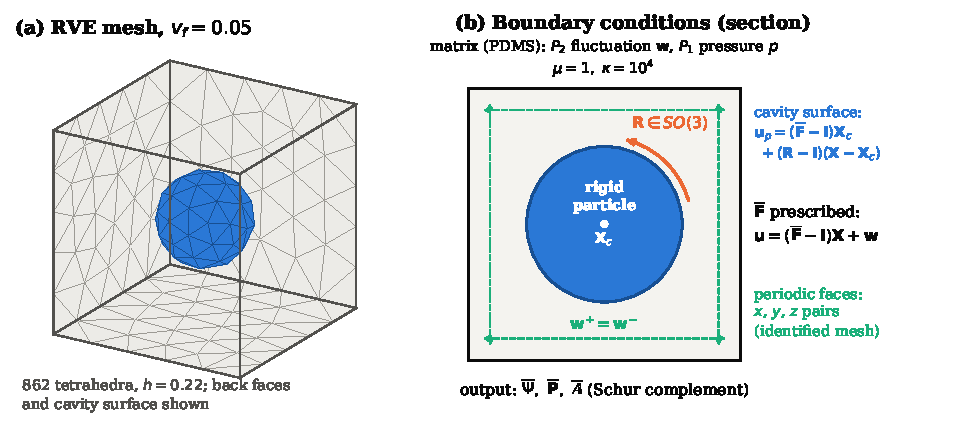
\includegraphics[width=\textwidth]{fig_rve_setup.pdf}
\caption[RVE finite-element model]{RVE finite-element model. (a) Netgen mesh of the matrix for $\vfrac=0.05$; the
particle is not meshed, only its cavity surface (blue) carries the rigid trace. Back
faces shown; opposite faces have identical surface meshes. (b) Section through the
RVE: periodic fluctuation $\bm w$ on all three face pairs, exact rigid motion of the
cavity surface with rotation $\Rten$ from moment equilibrium, and macroscopic
deformation $\Fbar$ imposed through \cref{eq:kin}.}
\label{fig:rvesetup}
\end{figure}

{\small
\begin{xltabular}{\textwidth}{@{}p{3.6cm}X@{}}
\caption{Microscale (RVE) finite-element setup used for all datasets.}\label{tab:micro}\\
\toprule
Item & Setting\\
\midrule
\endfirsthead
\caption[]{\emph{(continued)}}\\
\toprule
Item & Setting\\
\midrule
\endhead
\bottomrule
\endfoot
Domain & unit cube $[0,1]^3$ with centred spherical cavity, radius $r=(3\vfrac/4\pi)^{1/3}$ (0.168, 0.229, 0.288)\\
Geometry and mesh & Netgen OCC kernel, opposite faces identified before meshing; unstructured tetrahedra, $h=0.22$; boundaries \code{xmin}, \dots, \code{zmax}, \code{particle}\\
Mesh size per $\vfrac$ & 1441 / 862 / 875 tetrahedra for $\vfrac=0.02/0.05/0.10$\\
Elements & Taylor--Hood: $P_2$ periodic vector displacement fluctuation, $P_1$ periodic pressure\\
Degrees of freedom & 7518 / 5043 / 5102 in total, 5654 / 3275 / 3310 free after periodic and rigid-trace constraints; plus 3 rotation unknowns\\
Quadrature & integration order 10 in all volume and surface forms\\
Matrix material & mixed near-incompressible neo-Hookean, \cref{eq:mixed}: $\mu=1$, $\kappa=10^4$\\
Particle & exactly rigid: Dirichlet trace \cref{eq:rigid} on \code{particle}; free rotation from moment equilibrium\\
Kinematic loading & prescribed $\Fbar$ through $\F=\Fbar+\nabla\bm w$; translation gauge fixed\\
Nonlinear solver & Newton with exact symbolic Jacobian and backtracking line search with $J>0$ check; tolerance $10^{-8}$ (residual), $10^{-9}$ (moment); adaptive load continuation\\
Linear solver & sparse direct factorization (UMFPACK~\cite{Davis2004})\\
Homogenized tangent & 9 macroscopic + 3 rotational \code{NumberSpace} unknowns; one factorization, Schur complement \cref{eq:schur}\\
\end{xltabular}
}

\paragraph{Mesh and quadrature convergence.} The production resolution was chosen by
a convergence study (\code{rve\_phase2\_convergence.json}) before any dataset was
generated. Eight macroscopic states (hydrostatic tension and compression, uniaxial
and biaxial tension, simple shear, a combined non-symmetric state and two boundary
states of the sampling domain) were solved at $\vfrac=0.02$ and $0.10$ on three
meshes ($h=0.30$, $0.22$, $0.16$) with integration orders 6 and 10. Energy, stress
and tangent were compared with the finest solution ($h=0.16$, order~10), and
accuracy targets of $0.2\,\%$, $0.5\,\%$ and $1\,\%$ were set in advance.
\Cref{fig:rveconv} gives the largest error over the eight states. The coarse mesh
misses the energy and stress targets for simple shear at $\vfrac=0.10$
($7.1\times10^{-3}$ and $7.5\times10^{-3}$); $h=0.22$ satisfies all targets, the energy target with a
margin of a factor of 2.6. At $\vfrac=0.10$ the remaining error of
$7.7\times10^{-4}$ is the same for energy, stress and tangent, for every state and
for both coarser meshes, except for simple shear, whose energy and stress errors at
$h=0.22$ are $5.7\times10^{-4}$ and $7.5\times10^{-4}$. Such a
uniform relative offset points to the polyhedral approximation of the particle
surface, which changes the effective volume fraction slightly, rather than to the
resolution of the displacement field. The integration order has no visible
effect (order~6 versus 10 at $h=0.16$: below $10^{-9}$). Order~10 was nevertheless
kept for production as a conservative choice.

\begin{figure}[htbp]
\centering
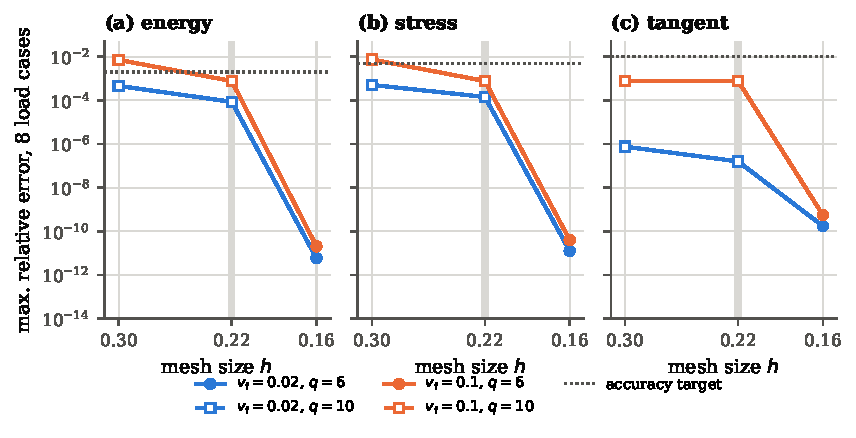
\includegraphics[width=\textwidth]{fig_rve_convergence.pdf}
\caption[RVE mesh and quadrature convergence]{RVE mesh and quadrature convergence: largest relative error of the
homogenized (a) energy, (b) stress and (c) tangent over eight load states, relative
to the solution with $h=0.16$ and integration order~10. Dotted: accuracy target set
before the study. Grey band: production mesh $h=0.22$. Points at $h=0.16$ compare
integration order 6 with 10 only.}
\label{fig:rveconv}
\end{figure}

\section{Dataset generation}

Deformation gradients are drawn by a seeded uniform perturbation of $\Iten$ and
filtered for $J>0$ and a bounded condition number. Targeted campaigns add
stratified compression ($J\in[0.51,0.60]$) and expansion ($J\in[1.50,1.80]$)
states. Every deformation state is solved at all three volume fractions, and the
whole \emph{group} is assigned to the training, validation or test split. This
prevents the same loading from appearing in two splits. A record is accepted
only if the mixed, rotational and condensed residuals are below $10^{-8}$, the
minimum microscopic $J$ exceeds its floor, the particle clearance is positive and
all arrays are finite. Per-sample results are written atomically, so an
interrupted cluster job resumes without trusting partial files. A JSON manifest
records the configuration, schema, software versions, split counts and SHA-256
hashes. \Cref{tab:datasets} lists the datasets.

{\small
\begin{xltabular}{\textwidth}{@{}lrX@{}}
\caption[Direct-RVE datasets]{Direct-RVE datasets (each record: $\Fbar$, $\vfrac$, $\Psibar$, $\Pbar$, $\Abar$, $\Rten$, residuals, diagnostics).}\label{tab:datasets}\\
\toprule
Dataset & Records & Purpose\\
\midrule
\endfirsthead
\caption[]{\emph{(continued)}}\\
\toprule
Dataset & Records & Purpose\\
\midrule
\endhead
\bottomrule
\endfoot
Phase 2 pilot & 300 & first schema; integrity and pipeline test\\
Phase 3 & 900 & intermediate dataset generated before the targeted sets\\
Phase 4 compression & 1080 & compressive states\\
Phase 5 independent & 360 & independently seeded set\\
Phase 6 targeted & 1260 & targeted sampling of the $J$ tails; stage-1 training data\\
Phase 7 independent & 600 & new seed; 531 eligible test records (33 train and 33 validation records of it entered stage~2)\\
Fresh holdout (\code{rve\_extra\_holdout}) & 90 & generated after the checkpoint was frozen; evaluation and timing benchmark\\
Shear adaptation & 33 & simple-shear fine-tuning data (18 train, 6 validation, 9 development test)\\
Shear context holdout & 15 & simple-shear cases used to compare the adaptation variants (\cref{sec:shearvariants})\\
Final shear holdout & 15 & 12 scored simple-shear cases, new microstructure seed\\
\end{xltabular}
}
The ten datasets hold 4653 distinct records. The stage-2 dataset
(\code{rve\_phase6\_phase7\_training}, 1671 records, split 909/225/537) is a composite
drawn from the Phase~6 and Phase~7 sets and adds no further records; the 189 Phase~6
test records are not part of it.

\section{Network architecture}\label{sec:architecture}

\Cref{fig:arch} shows the partially input-convex network implemented in
\code{src/picnn.py}. The deformation gradient enters only through the invariant
features $\bm y=[I_1,\,I_2,\,J,\,-\ln J]$, which makes the energy isotropic and
objective by construction. Features and context are standardized with fixed means
and positive scales from the training split, $\hat{\bm y}=(\bm y-\bm m_y)\oslash\bm s_y$
and $\hat c=(\vfrac-m_c)/s_c$; a positive affine scaling preserves convexity and
monotonicity. With $W^{+}=\mathrm{softplus}(W)$ and $\sigma=\mathrm{softplus}$, the
forward pass is
\begin{align}
  [\bm b_1,\bm b_2,\bm b_3] &= \bm V_2\,\sigma(\bm V_1\hat c+\bm\beta_{c1})+\bm\beta_{c2},\label{eq:ctx}\\
  \bm z_1 &= \sigma\bigl(W_{y,1}^{+}\hat{\bm y}+\bm\beta_1+\bm b_1\bigr),\\
  \bm z_l &= \sigma\bigl(W_{z,l}^{+}\bm z_{l-1}+W_{y,l}^{+}\hat{\bm y}+\bm\beta_l+\bm b_l\bigr),\qquad l=2,3,\\
  \Psi_{\mathrm{raw}} &= \bm w_{\mathrm{out}}^{+}\cdot\bm z_3+\beta_{\mathrm{out}},
\end{align}
followed by the reference normalization \cref{eq:norm}. All weights acting on
$\hat{\bm y}$ or on hidden states are non-negative and $\sigma$ is convex and
non-decreasing, so $\Psi_{\mathrm{raw}}$ is convex and non-decreasing in $\hat{\bm y}$
for every $\vfrac$. The context network \cref{eq:ctx} is unconstrained, because it only
shifts biases. The passthrough connections $W_{y,l}^{+}\hat{\bm y}$ let every layer see
the features directly, as proposed for ICNNs~\cite{Amos2017}. The positive weights
are initialized such that $\mathrm{softplus}(W)\approx0.05$ ($W_y$, $\bm w_{\mathrm{out}}$)
and $0.02$ ($W_z$), which avoids the overly stiff initial energy that
$\mathrm{softplus}(0)\approx0.69$ would produce. Stress and tangent are obtained by
automatic differentiation of $\widehat\Psi$ with respect to $\F$. \Cref{tab:params}
lists all trainable parameters.

\paragraph{How weights and biases are chosen.} None of the 5793 parameters is set by
hand; all are found by the training described in \cref{sec:training}. Only their
starting values and constraints are prescribed. Each constrained weight is stored as an
unconstrained raw value $W$ and enters the network as $\mathrm{softplus}(W)$, so any
raw value yields a non-negative effective weight. The raw values are drawn from a
normal distribution with standard deviation $0.05$ around
$\log(e^{w_0}-1)$, which makes the effective weight start near $w_0=0.05$
($W_y$, $\bm w_{\mathrm{out}}$) or $0.02$ ($W_z$). The biases $\bm\beta_{1..3}$ and
$\beta_{\mathrm{out}}$ start at zero. The unconstrained context network uses the default
PyTorch initialization of linear layers, a uniform distribution scaled by the layer
width. The random number generator is seeded: $2719$ for stage~1, $4103$ for stage~2
and $20261116$ for the shear-adapted stage. Training results were not compared across
seeds, so the sensitivity of the final parameters to the seed is not quantified. The
architecture (three hidden layers of width $32$) and the optimizer settings of
\cref{tab:trainconf} were fixed in the training scripts and are the values used in the
final runs; no systematic hyperparameter search is reported here.

\begin{figure}[htbp]
\centering
\resizebox{\textwidth}{!}{%
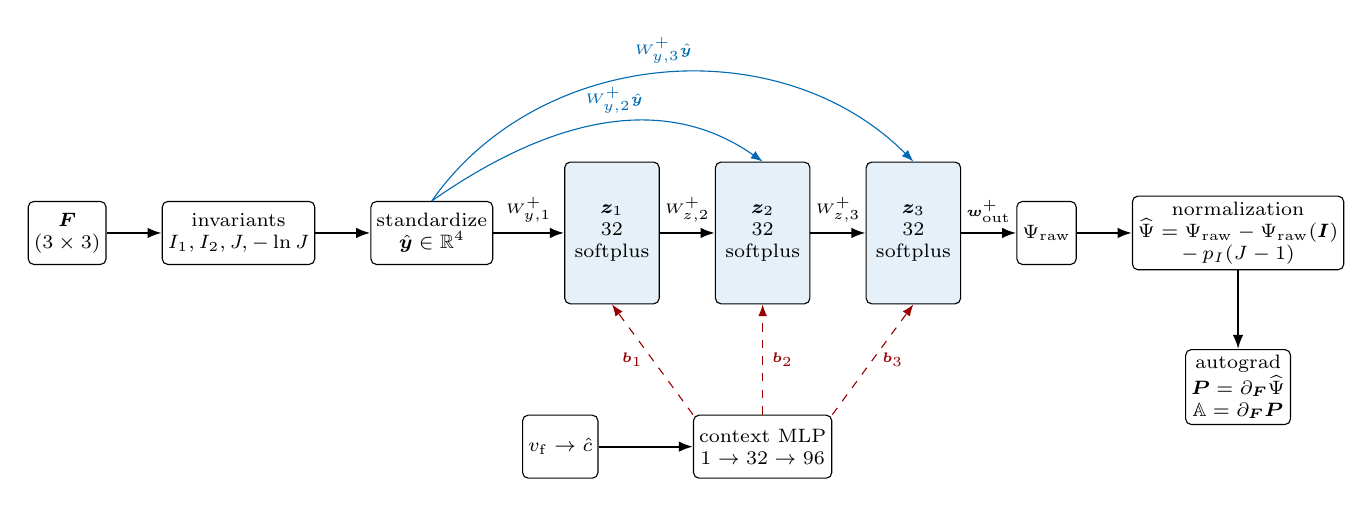
\begin{tikzpicture}[
  node distance=5mm and 7mm,
  blk/.style={draw, rounded corners=2pt, align=center, font=\scriptsize, minimum height=8mm, inner sep=2pt, fill=white},
  hid/.style={draw, fill=tubafblue!10, rounded corners=2pt, align=center, font=\scriptsize, minimum width=12mm, minimum height=18mm},
  arr/.style={-{Latex[length=1.8mm]}, thick},
  pas/.style={-{Latex[length=1.5mm]}, thin, tubafblue},
  ctx/.style={-{Latex[length=1.5mm]}, thin, red!60!black, dashed}]
  \node[blk] (F) {$\F$\\$(3\times3)$};
  \node[blk, right=of F] (inv) {invariants\\$I_1,I_2,J,-\ln J$};
  \node[blk, right=of inv] (std) {standardize\\$\hat{\bm y}\in\mathbb R^4$};
  \node[hid, right=9mm of std] (z1) {$\bm z_1$\\32\\softplus};
  \node[hid, right=of z1] (z2) {$\bm z_2$\\32\\softplus};
  \node[hid, right=of z2] (z3) {$\bm z_3$\\32\\softplus};
  \node[blk, right=of z3] (out) {$\Psi_{\mathrm{raw}}$};
  \node[blk, right=of out] (nrm) {normalization\\$\widehat\Psi=\Psi_{\mathrm{raw}}-\Psi_{\mathrm{raw}}(\Iten)$\\$-\,p_I(J-1)$};
  \node[blk, below=10mm of nrm] (ad) {autograd\\$\Pstress=\partial_{\F}\widehat\Psi$\\$\Aten=\partial_{\F}\Pstress$};
  \node[blk, below=14mm of z2] (cn) {context MLP\\$1\to32\to96$};
  \node[blk, left=12mm of cn] (vf) {$\vfrac\to\hat c$};
  \draw[arr] (F)--(inv); \draw[arr] (inv)--(std); \draw[arr] (std)--node[above,font=\tiny]{$W_{y,1}^+$}(z1);
  \draw[arr] (z1)--node[above,font=\tiny]{$W_{z,2}^+$}(z2); \draw[arr] (z2)--node[above,font=\tiny]{$W_{z,3}^+$}(z3);
  \draw[arr] (z3)--node[above,font=\tiny]{$\bm w^+_{\mathrm{out}}$}(out); \draw[arr] (out)--(nrm); \draw[arr] (nrm)--(ad);
  \draw[pas] (std.north) to[out=35,in=145] node[pos=0.55,above,font=\tiny]{$W_{y,2}^+\hat{\bm y}$} (z2.north);
  \draw[pas] (std.north) to[out=55,in=135] node[pos=0.5,above,font=\tiny]{$W_{y,3}^+\hat{\bm y}$} (z3.north);
  \draw[arr] (vf)--(cn);
  \draw[ctx] (cn.north west) -- node[left,font=\tiny]{$\bm b_1$} (z1.south);
  \draw[ctx] (cn.north) -- node[right,font=\tiny]{$\bm b_2$} (z2.south);
  \draw[ctx] (cn.north east) -- node[right,font=\tiny]{$\bm b_3$} (z3.south);
\end{tikzpicture}}
\caption[Architecture of the volume-fraction-conditioned pICNN]{Architecture of the volume-fraction-conditioned pICNN. Solid black: convex,
non-decreasing path with non-negative weights; blue: input passthrough; dashed red:
unconstrained context network producing layer biases.}
\label{fig:arch}
\end{figure}

\begin{table}[htbp]
\centering\small
\caption{Trainable parameters of the pICNN (\code{HyperelasticNN(n\_ctx=1)}).}
\label{tab:params}
\begin{tabular}{@{}llrl@{}}
\toprule
Block & Shape & Parameters & Constraint\\
\midrule
input passthrough $W_{y,1..3}$ & $3\times(32\times4)$ & 384 & softplus $\ge0$\\
hidden-to-hidden $W_{z,2},W_{z,3}$ & $2\times(32\times32)$ & 2048 & softplus $\ge0$\\
biases $\bm\beta_{1..3}$ & $3\times32$ & 96 & none\\
output $\bm w_{\mathrm{out}}$, $\beta_{\mathrm{out}}$ & $32+1$ & 33 & softplus $\ge0$ / none\\
context $\bm V_1,\bm\beta_{c1}$ & $32\times1+32$ & 64 & none\\
context $\bm V_2,\bm\beta_{c2}$ & $96\times32+96$ & 3168 & none\\
\midrule
total & & 5793 & (2561 without context, Phase~1)\\
\bottomrule
\end{tabular}
\end{table}

\section{Surrogate training}\label{sec:training}

Training (\code{src\slash{}train\_rve.py}) runs in float64 with Adam~\cite{Kingma2015}
with batches of 64 and a learning rate of $10^{-3}$ in stage~1 and $10^{-4}$ in stage~2.
Input features and context are standardized with
statistics of the training split only. The loss is
\begin{equation}
  \mathcal L=\Bigl\langle\Bigl(\frac{\widehat\Psi-\Psibar}{s_\Psi}\Bigr)^2\Bigr\rangle
  +w_P\Bigl\langle\Bigl(\frac{\widehat P_{iJ}-\overline P_{iJ}}{s_P}\Bigr)^2\Bigr\rangle
  +w_A\Bigl\langle\frac{\|\widehat{\Aten}-\Abar\|_F^2}{\|\Abar\|_F^2}\Bigr\rangle ,
  \label{eq:loss}
\end{equation}
with $w_P=1$ and $w_A=0.1$. The tangent term is evaluated on sub-batches of 8
states (half with $J<0.7$), because second derivatives are memory-intensive.
Following the Sobolev-training idea~\cite{Czarnecki2017}, energy and its
derivatives are matched simultaneously. The scales $s_\Psi$ and $s_P$ are the
root-mean-square values of energy and stress components over the training split:
$s_\Psi=979$ and $s_P=2440$. These are the values of the Phase~6 training split
(stage~1); they were kept fixed in stages~2 and~3 (the Phase~6/7 training split would give
991 and 2469). The epoch is selected by
validation loss with patience. The frozen checkpoint (SHA-256 prefix
\code{32b0a41f}, epoch 2750) was fine-tuned from the Phase~6 model on the merged
Phase~6/7 data. A second, \emph{shear-adapted} checkpoint (prefix
\code{5c1c6060}, epoch 275) was fine-tuned on the shear-adaptation data with the
original data replayed.

{\small
\begin{xltabular}{\textwidth}{@{}p{4.1cm}XXX@{}}
\caption[Training configuration of the three stages]{Training configuration of the frozen checkpoint (stages 1 and 2) and of the shear-adapted checkpoint (stage 3).}\label{tab:trainconf}\\
\toprule
Setting & Stage 1 (Phase 6 data) & Stage 2 (Phase 6/7 data) & Stage 3 (shear-adapted)\\
\midrule
\endfirsthead
\caption[]{\emph{(continued)}}\\
\toprule
Setting & Stage 1 (Phase 6 data) & Stage 2 (Phase 6/7 data) & Stage 3 (shear-adapted)\\
\midrule
\endhead
\bottomrule
\endfoot
precision, device & \multicolumn{3}{l}{float64, CPU}\\
optimizer & \multicolumn{3}{l}{Adam}\\
learning rate & $10^{-3}$ & $10^{-4}$ & $2\times10^{-5}$\\
initialized from & random (\cref{sec:architecture}) & stage-1 model & frozen stage-2 model\\
max.\ epochs / selected & 3000 / 2500 & 3000 / 2750 & 500 / 275\\
validation interval; patience & 25 epochs; 20 checks & 25 epochs; 20 checks & 5 epochs; 20 checks\\
batch size & 64 & 64 & 64 original + 16 shear\\
tangent sub-batch & 8 (half with $J<0.7$) & 8 (half with $J<0.7$) & 8 original + 8 shear\\
loss weights & $w_P=1$, $w_A=0.1$ & $w_P=1$, $w_A=0.1$ & $w_A=0.1$ (original), $1$ (shear response), $1$ (shear tangent)\\
seed & 2719 & 4103 & 20261116\\
\end{xltabular}
}

Data splits are grouped by deformation state, so that all volume fractions of one
state fall into the same split (train / validation / test).

\paragraph{Shear-adapted stage.} The shear-adaptation dataset contains 33 simple-shear
records, split by deformation state into 18 training, 6 validation and 9 development-test
records. Stage~3 starts from the frozen checkpoint and replays the original training data
in every step, so that the response outside shear is not forgotten. Its loss adds a
shear-stress and energy term and a $\partial\overline P_{01}/\partial\overline F_{01}$
tangent term, each normalized by the RMS value of that quantity over the shear training
records. The checkpoint is selected by the equal-weighted mean of two ratios: the original
validation objective and the shear validation objective, each relative to the frozen
model. The selected epoch is therefore the one that improves shear without worsening the
original validation. \Cref{sec:shearvariants} reports the two other adaptation variants
that were trained from the same starting point.

\paragraph{Scale of the loss terms.} Both $s_\Psi$ and $s_P$ are dominated by the volumetric response
(\cref{sec:scales}): the pressure in a state with $J=0.55$ is of order $4500$,
while the deviatoric stress is of order $1$. Each term of \cref{eq:loss} is
therefore nearly blind to shear. \Cref{sec:diagnosis} quantifies this effect.

\section{Macroscopic finite-element solution}\label{sec:macro-method}

The component-scale problem (\code{benchmarks\slash{}phase6\_macro\_fe\_demo.py}) is the
unit cube with both end faces clamped: $\bm u=\bm 0$ on $x=0$ and
$\bm u=(\varepsilon,0,0)$ on $x=1$, all components prescribed, with the lateral
faces traction-free and $\vfrac=0.05$. The load is applied in 100 increments
(10--20 for the $P_2$ runs). Each increment is solved by the Phase~1 bridge, now
fed by the RVE-trained pICNN, with three globalization devices~\cite{Nocedal2006}:
\begin{itemize}
  \item a \emph{secant predictor} that extrapolates the displacement from the
        two previous converged increments;
  \item a \emph{backtracking line search} on the discrete potential energy
        (merit function) that also rejects any trial state with $J\le10^{-8}$;
  \item a \emph{spectrally shifted Newton} fallback,
        $(\bm K+\alpha\bm I)\Delta\bm u=-\bm R$ with $\alpha$ just above
        $-\lambda_{\min}(\bm K)$, when the line search stagnates.
\end{itemize}
Convergence is declared at $\|\bm R_{\mathrm{free}}\|<10^{-8}$. The
macroscopic problem has displacement unknowns only. The RVE pressure and
rotation have been eliminated in the homogenized law, so the workflow is offline
homogenization followed by a surrogate macro solve, not concurrent FE$^2$. \Cref{fig:macrosetup} shows the model and \cref{tab:macrosetup} lists the setup.

\begin{figure}[htbp]
\centering
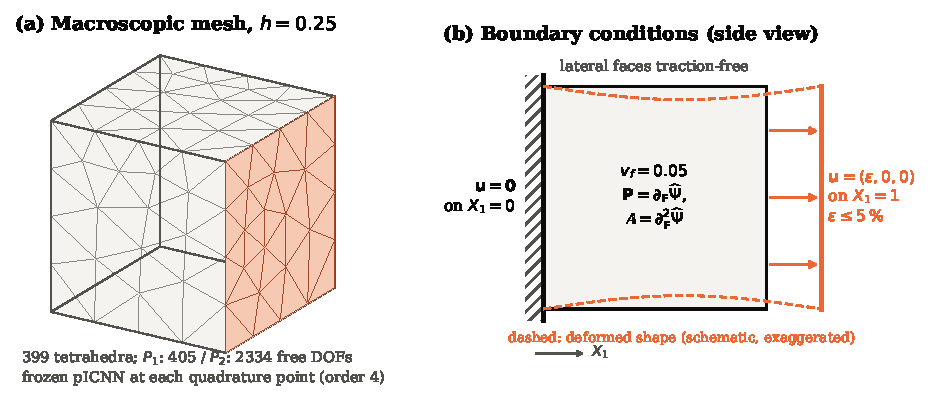
\includegraphics[width=\textwidth]{fig_macro_setup.pdf}
\caption[Macroscopic finite-element model]{Macroscopic finite-element model. (a) Unit-cube mesh for $h=0.25$; the
loaded face $X_1=1$ is shaded. (b) Boundary conditions: face $X_1=0$ clamped, face
$X_1=1$ displaced by $(\varepsilon,0,0)$ with lateral motion suppressed, lateral faces
traction-free. The frozen pICNN supplies stress and tangent at every quadrature
point.}
\label{fig:macrosetup}
\end{figure}

{\small
\begin{xltabular}{\textwidth}{@{}p{3.6cm}X@{}}
\caption{Macroscale finite-element setup.}\label{tab:macrosetup}\\
\toprule
Item & Setting\\
\midrule
\endfirsthead
\caption[]{\emph{(continued)}}\\
\toprule
Item & Setting\\
\midrule
\endhead
\bottomrule
\endfoot
Domain and mesh & unit cube (Netgen OCC), unstructured tetrahedra, $h=0.25/0.20/0.16$ with 399 / 648 / 1818 elements\\
Elements & vector Lagrange $P_1$ (405 / 642 / 1356 DOFs) or $P_2$ (2334 / 3759 / 8928 DOFs); displacement only\\
Quadrature & integration order 4 (46 points per tetrahedron; 18\,354 points at $h=0.25$), identical for $\bm R$, $\bm K$ and the material data\\
Material & frozen pICNN at $\vfrac=0.05$, evaluated at every quadrature point\\
Boundary conditions & $\bm u=\bm 0$ on $x=0$; $\bm u=(\varepsilon,0,0)$ on $x=1$; lateral faces traction-free\\
Loading & $\varepsilon=5\,\%$ in 100 increments ($P_1$); $0.5\,\%$ / $1\,\%$ in 10 / 20 increments ($P_2$)\\
Nonlinear solver & Newton with energy line search, secant predictor, spectral shift; tolerance $10^{-8}$\\
Linear solver & sparse direct factorization (UMFPACK)\\
\end{xltabular}
}


\chapter{Code(s) Available and Used}\label{ch:codes}

\section{Closest existing codes on the World Wide Web}

The guideline requires an explicit answer to the question of which existing
code comes closest to this project. A search over Python, Julia, MATLAB,
Fortran/Abaqus and C++ resources found \emph{no} public code that combines all
four ingredients of this project: (i) a periodic finite-strain RVE with an
exactly rigid, freely rotating inclusion; (ii) a condensed consistent tangent;
(iii) a polyconvex neural energy trained on that data; and (iv) deployment of the
network as a material law inside NGSolve. Each ingredient on its own, however,
has close precedents, summarized in \cref{tab:available}. The closest code to the
neural material law in NGSolve is the forum example~\cite{NGSolveForumTF}; the
closest RVE formulations are the COMET and Ferrite.jl homogenization examples.

{\small
\begin{xltabular}{\textwidth}{@{}p{3.1cm}p{1.9cm}X@{}}
\caption{Closest publicly available codes and their relation to this project.}\label{tab:available}\\
\toprule
Code & Language & Functionality and relation to this project\\
\midrule
\endfirsthead
\caption[]{\emph{(continued)}}\\
\toprule
Code & Language & Functionality and relation to this project\\
\midrule
\endhead
\bottomrule
\endfoot
COMET / comet-fenicsx tours~\cite{CometFenics} & Python (FEniCSx, \code{dolfinx\_mpc}) &
  Periodic homogenization of a 2D plane-strain \emph{linear} elastic composite with
  deformable circular inclusions; the periodic fluctuation is the unknown, as in
  \cref{eq:kin}. Closest RVE formulation, but small strain, two-dimensional, no
  rigid inclusion and no neural surrogate.\\
Ferrite.jl tutorial ``Computational homogenization''~\cite{Ferrite} & Julia &
  2D small-strain RVE with inclusions ten times stiffer than the matrix, Dirichlet and
  periodic boundary conditions. The homogenized stiffness follows from sensitivity
  fields for unit macroscopic strains with one reused factorization, the linear
  counterpart of the condensed tangent \cref{eq:schur}.\\
Andreassen \& Andreasen~\cite{Andreassen2014} & MATLAB &
  Short educational code for the homogenized elasticity tensor of periodic
  two-phase composites (small strain, voxel mesh).\\
EasyPBC~\cite{Omairey2019} & Python plug-in for Abaqus/CAE &
  Automatic periodic boundary conditions and effective elastic constants of
  user RVEs in Abaqus (linear elasticity).\\
MonolithFE$^2$~\cite{MonolithFE2} & Fortran (Abaqus UMAT/UEL) &
  Open-source FE$^2$ toolbox from TU Bergakademie Freiberg with monolithic and
  staggered algorithms and periodic micro boundary conditions. It solves the micro
  problem concurrently instead of using an offline surrogate, and is the reference
  point for the concurrent alternative discussed in \cref{ch:intro}.\\
CANN~\cite{Linka2021} & Python (TensorFlow) &
  Constitutive artificial neural networks for hyperelasticity trained on stress
  data; invariant-based, physics-structured, but not coupled to an FE solver in
  the public code and not trained on RVE data.\\
Physics-augmented NNs~\cite{Klein2022,Linden2023,Kalina2022} & method papers &
  Polyconvex invariant-based ICNN energies with stress normalization; the
  methodological basis of the pICNN (features, non-negative weights,
  normalization). Not a reusable package for NGSolve.\\
NGSolve i-tutorial 10.2 ``NGSolve with tensor-flow''~\cite{NGSolveTF} & Python (NGSolve + Keras/TensorFlow) &
  The precedent named by the committee. NGSolve solves a Poisson problem on a
  domain deformed by two parameters; a Keras network is trained to map the
  parameters to the nodal solution and is compared with a new NGSolve solve. Same
  offline-surrogate idea (FE data generation, then training), but the network
  replaces the whole solution and is not evaluated inside the FE solver.\\
NGSolve forum example~\cite{NGSolveForumTF} & Python (NGSolve + TensorFlow) &
  \emph{Closest code to the material-law coupling}: a trained network for the
  strain energy as a function of the Green--Lagrange strain is rebuilt from its
  weights as NGSolve coefficient functions and used in a nonlinear elasticity
  solve, with stresses from symbolic differentiation. The reported nonzero energy
  in the undeformed state is the defect removed by the normalization
  \cref{eq:norm}. No PyTorch, no quadrature-point transfer, no RVE data.\\
DNN in sequential multiscale FE~\cite{Troeger2023} & Python surrogate in Fortran FE &
  A purely data-based DNN surrogate of the RVE response (tangent by reverse-mode
  AD), integrated into a Fortran FE code and used in load-step-controlled simulations
  (2D plane strain, small strain). Reported speed-ups over FE$^2$ are 524$\times$
  (TensorFlow) and 6048$\times$ (JAX with just-in-time compilation) for a plate with a hole;
  these are not comparable with the present figures (other problem, hardware and
  reference). Same offline-surrogate idea; different strain regime, no physics
  constraints, other software.\\
\end{xltabular}
}

\section{Code(s) used in original or adapted form}

No source file of the codes in \cref{tab:available} was copied. The following
parts were used or adapted, as declared in the source documentation.

{\small
\begin{xltabular}{\textwidth}{@{}p{3.4cm}p{2.2cm}X@{}}
\caption{Software used in original or adapted form.}\label{tab:adapted}\\
\toprule
Source & Form & Use in this project\\
\midrule
\endfirsthead
\caption[]{\emph{(continued)}}\\
\toprule
Source & Form & Use in this project\\
\midrule
\endhead
\bottomrule
\endfoot
NGSolve periodicity tutorial~\cite{NGSolvePeriodic} & adapted &
  Face identification before meshing and the \code{Periodic} space wrapper
  (\code{src\slash{}rve.py}, \code{src\slash{}mixed\_matrix.py}).\\
NGSolve API (\code{IntegrationRuleSpace}, \code{NumberSpace}, symbolic forms) & original library &
  Quadrature-point data transfer, global macroscopic coordinates, exact
  linearization of the RVE residual.\\
ICNN architecture~\cite{Amos2017} & re-implemented &
  Non-negative hidden weights through softplus and input passthrough at every
  layer (\code{src\slash{}picnn.py}).\\
Invariant features and normalization~\cite{Linden2023,Klein2022} & adapted &
  Feature set $[I_1,I_2,J,-\ln J]$ and stress-free normalization, here in the
  objective pressure form \cref{eq:norm}.\\
PyTorch (\code{nn.Module}, \code{autograd}, \code{torch.func}, Adam) & original library &
  Network definition, AD stress and tangent, training loops.\\
Netgen OCC geometry kernel & original library & Cube with spherical cavity.\\
\end{xltabular}
}

\section{Original contributions}\label{sec:contrib}

The codes in \cref{tab:available} served as references for individual ideas; none
of their source was copied, and none provides any of the components below. The
project code (\RepositoryURL) comprises about 17\,000 non-blank, non-comment lines of
Python in \code{src/}, \code{tests/} (18 verification scripts) and \code{benchmarks/}
(20 study scripts). \Cref{tab:contrib} lists the components written for this project,
the closest precedent of each and what is new.

{\small
\begin{xltabular}{\textwidth}{@{}>{\raggedright\arraybackslash}p{3.0cm}>{\raggedright\arraybackslash}p{3.1cm}>{\raggedright\arraybackslash}X>{\raggedright\arraybackslash}p{1.5cm}@{}}
\caption[Components developed in this project]{Components developed in this project. Lines: non-blank, non-comment lines of the main module(s).}\label{tab:contrib}\\
\toprule
Component & Module(s), lines & New compared with the closest precedent & Verified by\\
\midrule
\endfirsthead
\caption[]{\emph{(continued)}}\\
\toprule
Component & Module(s), lines & New compared with the closest precedent & Verified by\\
\midrule
\endhead
\bottomrule
\endfoot
PyTorch--NGSolve material bridge &
  \code{ngsolve\_umat.py} (939) &
  The forum example~\cite{NGSolveForumTF} rebuilds a fixed network as symbolic
  coefficient functions. Here the PyTorch model is evaluated batch-wise at all
  quadrature points through \code{IntegrationRuleSpace}; stress and the full
  $9\times9$ AD tangent are returned to NGSolve, with energy line search, secant
  predictor and spectral shift. & V0a--e, V1, V4--V8, M-V0\\
Constrained energy network &
  \code{picnn.py} (171) &
  ICNN~\cite{Amos2017} with invariant features~\cite{Linden2023,Klein2022}; added
  volume-fraction context and the objective pressure normalization \cref{eq:norm}. & V2, V2b, V3, V0d, S-V1\\
Periodic mixed RVE with exactly rigid particle &
  \code{rve.py}, \code{mixed\_matrix.py}, \code{rve\_solver.py} (594) &
  COMET~\cite{CometFenics} and Ferrite.jl~\cite{Ferrite} treat small-strain elastic
  inclusions. Here: finite strain, Taylor--Hood $u$--$p$ matrix, rigid trace
  \cref{eq:rigid} imposed exactly, load continuation. & P2-V1--V4, P2-V8\\
Free particle rotation &
  \code{free\_particle.py} (569) &
  No precedent found: rotation as global unknown on $SO(3)$, condensed rotational
  Newton system from moment equilibrium. & P2-V2, P2-V7\\
Work-conjugate homogenization &
  \code{homogenization.py} (153) &
  Particle-reaction term of \cref{eq:hm}, required because the particle is a
  constraint and not a material phase. & P2-V5\\
Consistent homogenized tangent &
  \code{rve\_tangent.py} (315) &
  Ferrite.jl uses linear sensitivity fields; here the finite-strain Schur complement
  \cref{eq:schur} including the rotational unknowns. & P2-V6, P2-V9\\
Dataset generation and audit &
  \code{rve\_dataset.py}, \code{generate\_rve\_dataset\_parallel.py},
  \code{audit\_rve\_dataset.py}, \code{merge\_rve\_training\_data.py} (1459) &
  Deterministic, checkpointed, parallel generation; splits grouped by deformation
  state; hash-based provenance and audit. & P2-V10\\
Training and fine-tuning &
  \code{train.py}, \code{train\_rve.py}, \code{train\_rve\_shear\_adaptation.py} (1630) &
  Energy--stress--tangent loss with training-split scaling, early stopping, frozen
  checkpoints, shear fine-tuning with data replay. & Sec.~\ref{sec:trainperf}\\
Macroscopic application &
  \code{phase6\_macro\_fe\_demo.py} (347) &
  Surrogate as material law in a 3D finite-strain macro problem, $P_1$ and $P_2$. & M-V0, Sec.~\ref{sec:macro}\\
Verification and benchmarks &
  \code{tests/}, \code{benchmarks/} &
  26 tests (\cref{tab:vmatrix}), micromechanics, timing and holdout studies. & --\\
\end{xltabular}
}

\section{External libraries and versions}

\begin{table}[htbp]
\centering\small
\caption[External software]{External software. ``Cluster'' denotes the environment of all production runs; ``Local'' the clean environment of the final test runs and timing study.}
\label{tab:versions}
\begin{tabular}{@{}llll@{}}
\toprule
Software & Role & Cluster (production) & Local (final tests)\\
\midrule
Python & language & 3.11.7 & 3.13.18\\
NGSolve / Netgen & FEM, geometry, symbolic forms & 6.2.2608 & 6.2.2608\\
PyTorch & network, AD, training & 2.15.0+cpu & 2.15.0 (CPU use)\\
NumPy & arrays & 2.4.6 & 2.5.3\\
Matplotlib & plots & 3.11.0 (Phase 1) & 3.11.2\\
\bottomrule
\end{tabular}
\end{table}

All packages are freely available from PyPI (\code{pip install ngsolve torch
numpy matplotlib}); \code{requirements.txt} in the repository lists minimum
versions (\cref{ch:manual}).

\chapter{Program Flowchart and Software Architecture}\label{ch:flow}

\Cref{fig:flow} shows the complete workflow. The offline part produces and
audits data and trains the surrogate; the online part uses the frozen surrogate
as a material law. The two parts communicate only through two files with
SHA-256 hashes: the dataset (\code{.npz} with its manifest) and the checkpoint
(\code{.pt}).

\begin{figure}[htbp]
\centering
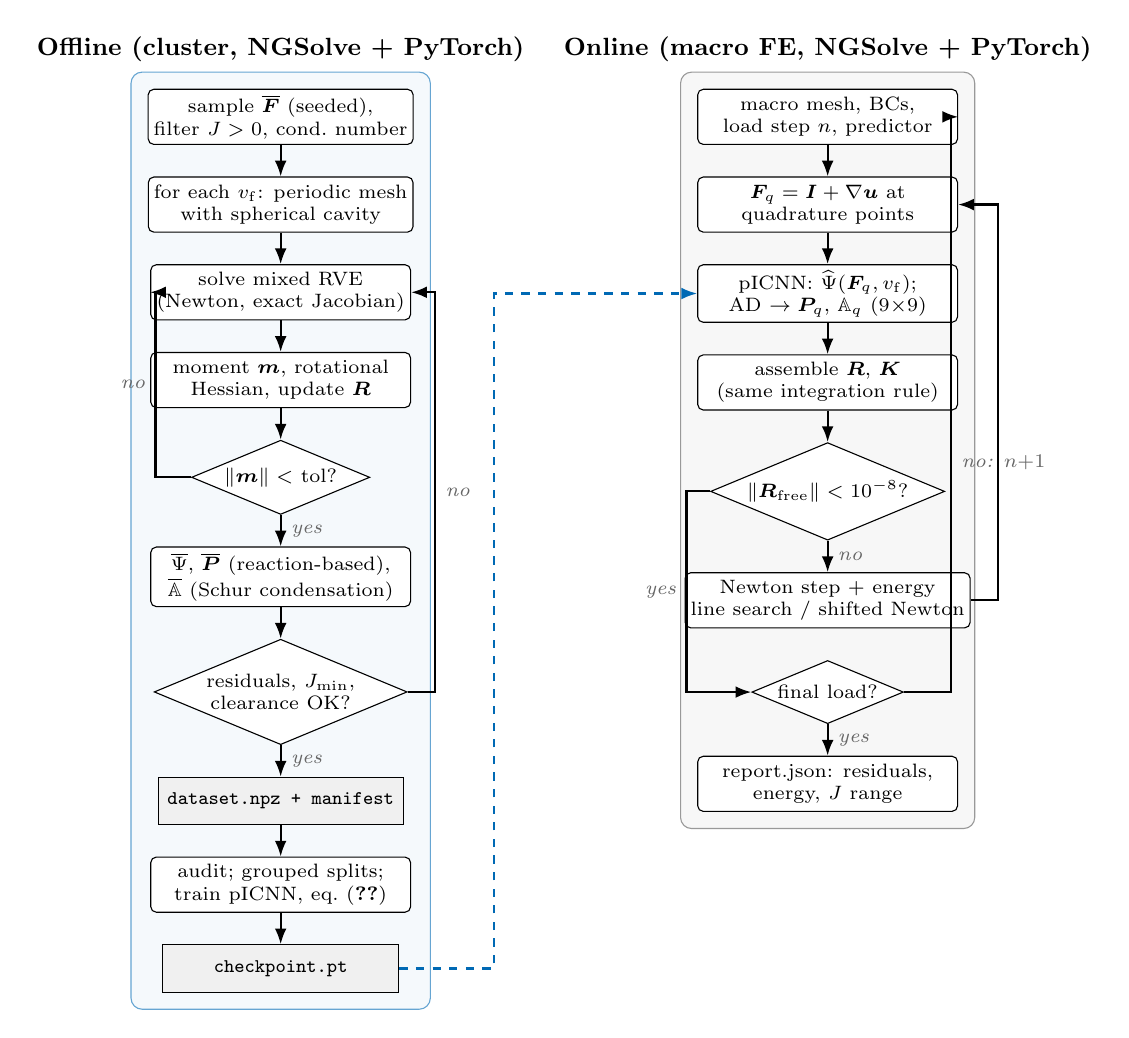
\begin{tikzpicture}[
  node distance=4mm and 6mm,
  box/.style={draw, rounded corners=2pt, fill=white, align=center, font=\scriptsize, minimum width=3.3cm, minimum height=7mm, inner sep=2pt},
  dec/.style={draw, diamond, aspect=2.4, fill=white, align=center, font=\scriptsize, inner sep=1pt},
  file/.style={draw, fill=black!6, align=center, font=\scriptsize\ttfamily, minimum width=3.0cm, minimum height=6mm},
  arr/.style={-{Latex[length=2mm]}, thick},
  lab/.style={font=\scriptsize\itshape, text=black!60}]
  % offline column
  \node[box] (s1) {sample $\Fbar$ (seeded),\\filter $J>0$, cond.\ number};
  \node[box, below=of s1] (s2) {for each $\vfrac$: periodic mesh\\with spherical cavity};
  \node[box, below=of s2] (s3) {solve mixed RVE\\(Newton, exact Jacobian)};
  \node[box, below=of s3] (s4) {moment $\bm m$, rotational\\Hessian, update $\Rten$};
  \node[dec, below=of s4] (d1) {$\|\bm m\|<$ tol?};
  \node[box, below=of d1] (s5) {$\Psibar$, $\Pbar$ (reaction-based),\\$\Abar$ (Schur condensation)};
  \node[dec, below=of s5] (d2) {residuals, $J_{\min}$,\\clearance OK?};
  \node[file, below=of d2] (f1) {dataset.npz + manifest};
  \node[box, below=of f1] (s6) {audit; grouped splits;\\train pICNN, eq.~\eqref{eq:loss}};
  \node[file, below=of s6] (f2) {checkpoint.pt};
  \draw[arr] (s1)--(s2); \draw[arr] (s2)--(s3); \draw[arr] (s3)--(s4); \draw[arr] (s4)--(d1);
  \draw[arr] (d1)--node[right,lab]{yes}(s5); \draw[arr] (s5)--(d2);
  \draw[arr] (d2)--node[right,lab]{yes}(f1); \draw[arr] (f1)--(s6); \draw[arr] (s6)--(f2);
  \draw[arr] (d1.west) -- ++(-0.45,0) |- node[pos=0.25,left,lab]{no} (s3.west);
  \draw[arr] (d2.east) -- ++(0.35,0) |- node[pos=0.25,right,lab]{no} (s3.east);
  % online column
  \node[box, right=3.6cm of s1] (m1) {macro mesh, BCs,\\load step $n$, predictor};
  \node[box, below=of m1] (m2) {$\F_q=\Iten+\nabla\bm u$ at\\quadrature points};
  \node[box, below=of m2] (m3) {pICNN: $\widehat\Psi(\F_q,\vfrac)$;\\AD $\to\Pstress_q$, $\Aten_q$ (9$\times$9)};
  \node[box, below=of m3] (m4) {assemble $\bm R$, $\bm K$\\(same integration rule)};
  \node[dec, below=of m4] (d3) {$\|\bm R_\mathrm{free}\|<10^{-8}$?};
  \node[box, below=of d3] (m5) {Newton step + energy\\line search / shifted Newton};
  \node[dec, below=of m5] (d4) {final load?};
  \node[box, below=of d4] (m6) {report.json: residuals,\\energy, $J$ range};
  \draw[arr] (m1)--(m2); \draw[arr] (m2)--(m3); \draw[arr] (m3)--(m4); \draw[arr] (m4)--(d3);
  \draw[arr] (d3)--node[right,lab]{no}(m5);
  \draw[arr] (m5.east) -- ++(0.35,0) |- (m2.east);
  \draw[arr] (d3.west) -- ++(-0.3,0) |- node[pos=0.25,left,lab]{yes} (d4.west);
  \draw[arr] (d4)--node[right,lab]{yes}(m6);
  \draw[arr] (d4.east) -- ++(0.6,0) |- node[pos=0.2,right,lab]{no: $n{+}1$} (m1.east);
  \draw[arr, dashed, tubafblue] (f2.east) -| ++(1.2,0) |- (m3.west);
  % frames
  \begin{scope}[on background layer]
    \node[draw=tubafblue!60, fill=tubafblue!4, rounded corners, fit=(s1)(f2)(d2), inner sep=6pt, label={[font=\small\bfseries]above:Offline (cluster, NGSolve + PyTorch)}] {};
    \node[draw=black!40, fill=black!3, rounded corners, fit=(m1)(m6)(d3), inner sep=6pt, label={[font=\small\bfseries]above:Online (macro FE, NGSolve + PyTorch)}] {};
  \end{scope}
\end{tikzpicture}
\caption[Program flowchart]{Program flowchart. Left: offline RVE data generation and training.
Right: online macroscopic Newton solve with the frozen pICNN as material law.
The dashed arrow is the only coupling: the frozen checkpoint.}
\label{fig:flow}
\end{figure}

\section{Module responsibilities}

{\small
\begin{xltabular}{\textwidth}{@{}p{4.4cm}X@{}}
\caption[Principal modules of the repository]{Principal modules of the repository (\code{Project implementation plan (2)\slash{}}).}\label{tab:modules}\\
\toprule
Module & Responsibility\\
\midrule
\endfirsthead
\caption[]{\emph{(continued)}}\\
\toprule
Module & Responsibility\\
\midrule
\endhead
\bottomrule
\endfoot
\code{src\slash{}picnn.py} & ICNN/pICNN energy, input normalization, reference correction\\
\code{src\slash{}constitutive.py}, \code{src\slash{}neohooke.py} & AD stress/tangent helpers; analytical Phase~1 law and data\\
\code{src\slash{}ngsolve\_umat.py} & quadrature-point bridge, \code{assemble\_system}, globalized Newton \code{solve}\\
\code{src\slash{}train.py} & Phase~1 training and checkpoint loading\\
\code{src\slash{}rve.py} & periodic cell with cavity, rigid kinematics utilities\\
\code{src\slash{}mixed\_matrix.py} & Taylor--Hood mixed PDMS formulation\\
\code{src\slash{}rve\_solver.py}, \code{src\slash{}free\_particle.py} & coupled periodic RVE solve; free finite particle rotation\\
\code{src\slash{}homogenization.py} & homogenized energy, reaction-based stress, Hill--Mandel checks\\
\code{src\slash{}rve\_tangent.py} & Schur-condensed tangent incl.\ rotational condensation\\
\code{src\slash{}rve\_dataset.py}, \code{src\slash{}generate\_rve\_dataset*.py}, \code{src\slash{}audit\_rve\_dataset.py} & sampling, checkpointing, manifests, parallel campaigns, audit\\
\code{src\slash{}train\_rve*.py} & pICNN training, fine-tuning and shear adaptation\\
\code{benchmarks\slash{}} & macro-FE demo, evaluations, timing and diagnostic studies\\
\code{tests\slash{}} & verification tests V0--V6 and P2-V1--P2-V10 (\cref{ch:verification})\\
\code{*.pbs} & PBS job scripts of every cluster run\\
\end{xltabular}
}

\paragraph{Design decisions.} (i) The production code and the tests share the
same functions; there is no separate test copy of any routine, as the
guideline demands. For example, V0d calls the production
\code{assemble\_system}. (ii) The two derivative paths are deliberately
separate: PyTorch AD for the learned energy, NGSolve symbolic differentiation
for the RVE. Each path is verified on its own (V3 and P2-V6). (iii) Every cluster
run writes a JSON report containing hashes of its inputs, so that every number in
\cref{ch:assessment} can be traced to an artifact (\cref{app:repro}).

\chapter{Usage of Chatbots and Other Tools}\label{ch:chatbots}

ChatGPT and Codex (OpenAI) and Claude (Anthropic), all AI-based language models,
were used as supporting tools throughout this project for understanding technical
concepts, programming, and scientific writing. They were mainly used to understand
the theoretical foundations on which this project builds (\cref{ch:theory}):
polyconvexity and input-convex neural networks, periodic homogenization and the
Hill--Mandel condition, and the condensation of internal variables for a consistent
homogenized tangent. In addition, they were used to understand the NGSolve and
PyTorch interfaces that this project connects, in particular the
\code{IntegrationRuleSpace}, periodic and \code{NumberSpace} function spaces and the
automatic-differentiation interface of PyTorch (\cref{ch:methods}).

During implementation, these tools were used to discuss code structure, investigate
programming errors, and evaluate possible solutions. Specific attention was given to
the consistent transfer of stress and tangent between PyTorch and NGSolve at the
quadrature points, the work-conjugate homogenized stress including the particle
reactions (\cref{eq:hm}), the objective form of the reference normalization
(\cref{eq:norm}), and the globalization of the macroscopic Newton solver
(\cref{sec:macro-method}). The tools also assisted in preparing the PBS job scripts
for the TU~Freiberg cluster and in developing the verification test cases
(\cref{ch:verification}). All suggestions were critically reviewed against the
governing equations and the library documentation, and were tested before being
used in the project.

Furthermore, these tools helped improve the clarity of the report, correct
grammatical errors, and structure the chapters. Additional support was provided for
\LaTeX{} formatting, TikZ diagrams, the program flowchart (\cref{ch:flow}) and the
plotting scripts. All suggested content was carefully reviewed against the
implemented methods, their mathematical formulations, the stored results
(\cref{app:repro}) and the verification results (\cref{ch:verification}).

\chapter{Testing for Verification}\label{ch:verification}

This chapter addresses verification, that is, whether the code solves the stated
equations correctly. The comparison of the surrogate with direct RVE solutions is
presented in \cref{ch:assessment}; experimental validation was not part of the
project.

All tests use the production modules; no routine exists in a separate test copy.
The tests were run during development (Phase~1 locally, Phase~2 on the cluster)
and, for the final code state, the complete suite was executed with the frozen
checkpoints and datasets (Python~3.13.18, NGSolve~6.2.2608, PyTorch~2.15.0). All
tests passed; the values below are from this execution. The complete suite runs with one command
(\code{./run\_tests.sh}, \cref{ch:manual}). \Cref{tab:vmatrix} gives the overview. Guideline items that do not
apply are stated explicitly: the model is quasi-static and rate-independent, so
there is no time integration and the time-integration stability and
convergence-order tests are not applicable.

{\small
\begin{xltabular}{\textwidth}{@{}llXl@{}}
\caption[Verification matrix (26 tests)]{Verification matrix (26 tests). Type: M = mandatory test of the guideline,
S = standard benchmark, C = custom (project-specific). All tests passed.}\label{tab:vmatrix}\\
\toprule
ID & Type & Aim & Key result\\
\midrule
\endfirsthead
\caption[]{\emph{(continued)}}\\
\toprule
ID & Type & Aim & Key result\\
\midrule
\endhead
\bottomrule
\endfoot
V0a & M & partition of unity of the shape functions ($P_1$, $P_2$) & $|\sum N_i-1|\le2.2\times10^{-16}$\\
V0b & M & exact linear field and gradient ($B$-matrix check) & gradient error $\le4.0\times10^{-14}$\\
V0c & M & volume/area by quadrature of the Jacobian, affine map & error $2.2\times10^{-14}$\\
V0d & M & six zero eigenvalues of the element stiffness (tet, hex; $P_1$, $P_2$) & 6/6 zero modes, span error $\le2\times10^{-9}$\\
V0e & M & hourglass modes under one-point integration & 18 zero modes (6 rigid + 12)\\
V1 & C & constitutive API, shapes, dtypes & pass\\
V2 & C & $\widehat\Psi(\Iten)=0$, $\Pstress(\Iten)=\bm 0$ & exactly $0$\\
V2b & S & pICNN vs.\ analytical neo-Hookean response & $5.37/3.27/3.87\,\%$\\
V3 & M & AD tangent vs.\ central differences & min.\ error $2.3\times10^{-10}$\\
V4 & M & Newton convergence, nonlinear FE solve & empirical order $1.90$\\
V5 & M & affine patch test, unstructured mesh & $\|\bm R_\mathrm{free}\|=2.7\times10^{-16}$\\
V6 & S & matched analytical vs.\ neural FE solution & reaction error $13.4\,\%<15\,\%$\\
V7 & M & single element, full deformation control: stress and tangent (SVK, neo-Hooke) & stress $5.5\times10^{-15}$, tangent $1.7\times10^{-11}$\\
V8 & M & single element, stress control (uniaxial traction), SVK then neo-Hooke & stretches exact to $2\times10^{-15}$\\
P2-V1 & C & triple periodicity of the fluctuation space & jump $2.2\times10^{-16}$\\
P2-V2 & C & exact rigid kinematics (rank 6, finite rotation) & constraint residual $7.2\times10^{-18}$\\
P2-V3 & M & mixed patch at $\kappa/\mu=10^4$ & $p$ error $2.9\times10^{-13}$\\
P2-V4 & C & coupled periodic RVE equilibrium & residual $1.9\times10^{-14}$\\
P2-V5 & S & Hill--Mandel macro-homogeneity & $1.2\times10^{-15}$\\
P2-V6 & M & condensed tangent: symmetry, Taylor order & order $2.000$, sym.\ $3.0\times10^{-16}$\\
P2-V7 & C & free rotation: moment equilibrium, $\Rten\in SO(3)$ & 3 iterations, $\|\Rten^{\mathsf T}\Rten-\Iten\|=2.5\times10^{-16}$\\
P2-V8 & C & translation-gauge invariance & stress change $1.2\times10^{-15}$\\
P2-V9 & M & free-rotation tangent vs.\ re-solved central differences & error $5.2\times10^{-12}$\\
P2-V10 & C & deterministic dataset, leak-free splits & 0 leaks, regeneration error $0$\\
S-V1 & M & surrogate: energy gradient, tangent, objectivity & $\le4.9\times10^{-8}$\\
M-V0 & M & macroscopic tangent vs.\ directional differences & $6.5\times10^{-10}$\\
\end{xltabular}
}

\Cref{fig:voverview} plots the key error measure of every test on one scale.
Most tests reach round-off ($10^{-18}$--$10^{-13}$), because they check an
identity that holds exactly in exact arithmetic. Larger values appear only where
the test measures an approximation or a tolerance by design: the trained Phase~1
network against the analytical law (V2b, V6); finite differences against an exact
derivative (V3, P2-V9, S-V1, M-V0), whose error is set by the difference step; the
Newton stopping tolerance (V4); and the eigenvalue threshold that defines the
numerical null space (V0d). The boundary-value problem of each element-level test is drawn
next to its description; the RVE tests use the model of \cref{fig:rvesetup}.

\begin{figure}[H]
\centering
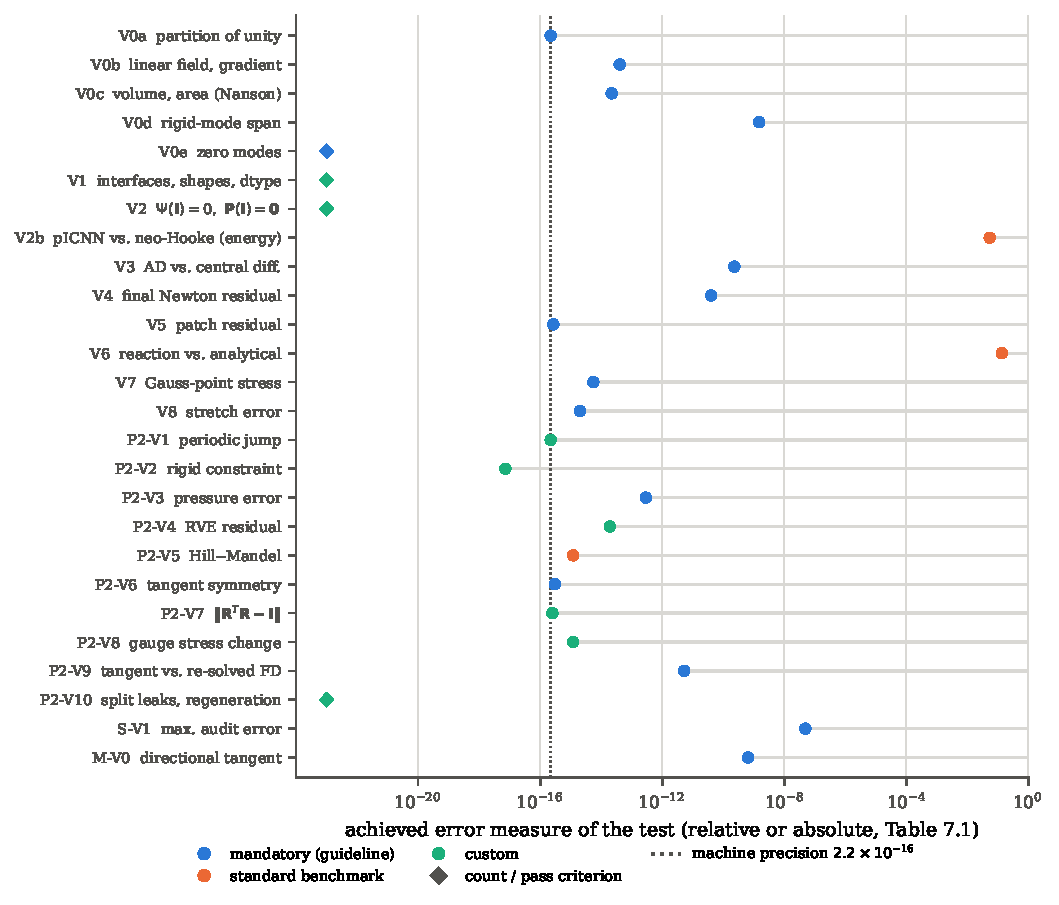
\includegraphics[width=\textwidth]{fig_v_overview.pdf}
\caption[Key error measure of all 26 verification tests]{Key error measure of all 26 verification tests (\cref{tab:vmatrix}).
Diamonds: tests with a count or a pass criterion instead of an error measure.
Dotted: machine precision $2.2\times10^{-16}$.}
\label{fig:voverview}
\end{figure}

% ======================================================================
\section{Finite-element basics}\label{sec:v0}

The NGSolve element library is heavily tested by its developers. The guideline
nevertheless requires these checks, because they also exercise \emph{this}
project's assembly path. All five are implemented in
\code{tests\slash{}verify\_fe\_basics.py} and use the production routine
\code{assemble\_system}.

\testcase{V0a/V0b}{Partition of unity and exact representation of linear fields}
\taim Verify $\sum_iN_i=1$ and $\sum_i\nabla N_i=\bm 0$, and that a linear field
and its gradient are reproduced exactly, for $P_1$ and $P_2$.
\tsetup Unstructured unit-cube mesh (112 tetrahedra, 55 vertices). NGSolve's $H^1$
basis is hierarchical, so the partition of unity is checked on the vertex
functions. The field is $0.4+0.3x-1.2y+0.7z$. The values are evaluated at one random interior point
per element (112 points).
\trun \code{python -m tests.verify\_fe\_basics}
\texpect Errors at round-off level ($\lesssim10^{-13}$).
\tobtain $|\sum N_i-1|=2.2\times10^{-16}$ and $|\sum\nabla N_i|=0$ for both orders.
Linear-field gradient errors are $2.4\times10^{-15}$ ($P_1$) and $4.0\times10^{-14}$
($P_2$). Pass.
\tinfer The element shape functions and gradients used by the production assembly are exact for linear fields, so no error enters the later tests from the interpolation itself.

\testcase{V0c}{Jacobian, volume and face area}
\taim Verify the element mapping Jacobian through numerical integration of
volume and area.
\tsetup Unit-cube mesh, deformed by the affine map with
$\bm F_a=\begin{bmatrix}1.10&0.05&0\\0.02&0.95&0.04\\0&0.03&1.07\end{bmatrix}$.
\texpect $V=\det\bm F_a=1.11576$; the area of the face $x=1$ follows Nanson's
formula, $A=\det\bm F_a\,\|\bm F_a^{-\mathsf T}\bm N\|=1.0167105$.
\tobtain $V=1.115760000000022$ and $A=1.016710548779736$. The maximum error is
$2.2\times10^{-14}$. Pass.
\tinfer The element mapping and its Jacobian are correct for an affine, non-symmetric map; volume and surface integrals, which enter the weak form and the traction terms, are exact to round-off.

\testcase{V0d}{Zero eigenvalues of the unconstrained element stiffness}
\taim A three-dimensional solid element must have exactly six zero-energy
modes at a stress-free state, namely three translations and three infinitesimal
rotations, and no others.
\tsetup One irregular tetrahedron and one distorted hexahedron, with $P_1$ and
$P_2$ displacements and full integration. The stiffness is assembled at
$\bm u=\bm 0$ without any boundary conditions, through the same
\code{assemble\_system} call that the Newton solver uses. Three materials are
used: the analytical neo-Hookean law \cref{eq:nh}, the frozen RVE-trained pICNN
($\vfrac=0.05$), and the legacy Phase~1 pICNN. An eigenvalue counts as zero if
$|\lambda|<10^{-9}\lambda_{\max}$; the smallest non-zero eigenvalue lies at least
two decades above this threshold in all cases.
\begin{figure}[H]
\centering
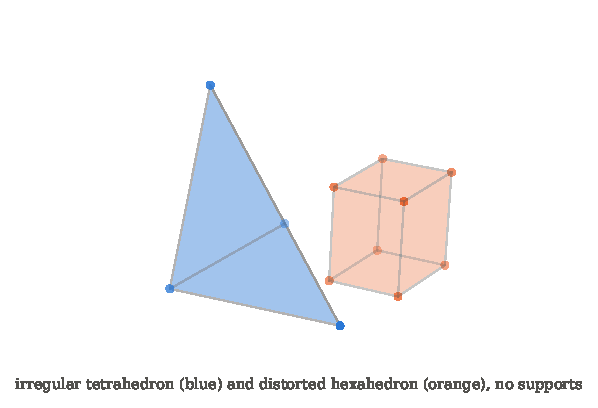
\includegraphics[width=0.4\textwidth]{fig_v_setup_v0.pdf}
\caption[V0d/V0e: boundary-value problem]{Boundary-value problem of V0d/V0e: one irregular tetrahedron and one distorted hexahedron, unconstrained.}
\label{fig:vsetup0}
\end{figure}

\trun \code{python -m tests.verify\_fe\_basics --ckpt checkpoints\slash{}phase1\_validated.pt --rve-ckpt <frozen.pt>}
\texpect Six zero eigenvalues, no negative ones, and a null space that contains
the six rigid-body vectors.
\tobtain See \cref{tab:v0d} and \cref{fig:v0spec}. The analytical law and the RVE pICNN pass in all
four element configurations: the rigid-body residual $\|\bm K\bm R\|$ is at
round-off, and the null space spans the rigid modes to $\le2\times10^{-9}$. The
legacy Phase~1 network, however, shows only \emph{three} zero eigenvalues and
\emph{three negative} ones. A rigid rotation of the unloaded body lowers its
energy. Evaluating the network directly confirms the cause predicted in
\cref{ch:theory}: for a rotation by $\theta$,
$\widehat\Psi(\Rten)=p_I\,(2-2\cos\theta)$ with $p_I=-0.2746$, to all printed
digits. This is the non-objective affine reference correction. It was removed
from Phase~5 onwards, which is why the production model passes. Tests V4--V6
could not detect the defect, because their Dirichlet boundaries suppress rigid
rotations. The Phase~1 gate verified the \emph{bridge}; it did not verify the
Phase~1 network as a frame-indifferent material.
\tinfer The assembly path produces the correct null space for the analytical law and for the production surrogate, so rigid motions cost no energy. The legacy Phase~1 network violates frame indifference and is therefore not a valid production model; this defect is invisible to tests with Dirichlet boundaries and is why the production energy is normalized objectively.

\begin{table}[H]
\centering\small
\caption[V0d/V0e: spectrum of the unconstrained element stiffness]{V0d/V0e: spectrum of the unconstrained element stiffness at $\F=\Iten$
(\code{assemble\_system}). $q$: NGSolve integration-rule order.}
\label{tab:v0d}
\begin{tabular}{@{}llrlrrrr@{}}
\toprule
Element & Order & $q$ & Material & DOFs & \#zero & \#neg. & $\|\bm K\bm R\|/(\|\bm K\|\|\bm R\|)$\\
\midrule
tet & 1 & 2 & neo-Hookean & 12 & 6 & 0 & $6.1\times10^{-17}$\\
tet & 1 & 2 & RVE pICNN & 12 & 6 & 0 & $5.7\times10^{-17}$\\
tet & 1 & 2 & Phase 1 pICNN (legacy) & 12 & \textbf{3} & \textbf{3} & $3.9\times10^{-3}$\\
tet & 2 & 4 & neo-Hookean / RVE pICNN & 30 & 6 & 0 & $\le1.2\times10^{-16}$\\
hex & 1 & 2 & neo-Hookean / RVE pICNN & 24 & 6 & 0 & $\le1.0\times10^{-16}$\\
hex & 2 & 4 & neo-Hookean / RVE pICNN & 81 & 6 & 0 & $\le2.5\times10^{-16}$\\
hex & 1 & 0 & neo-Hookean (one point) & 24 & \textbf{18} & 0 & $5.8\times10^{-17}$\\
\bottomrule
\end{tabular}
\end{table}

\begin{figure}[H]
\centering
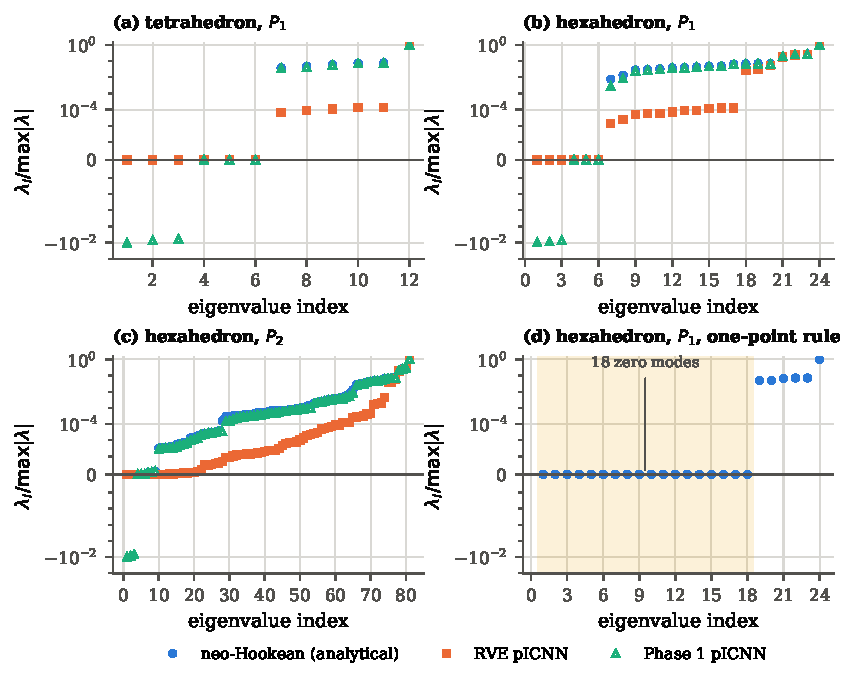
\includegraphics[width=\textwidth]{fig_v0_spectra.pdf}
\caption[V0d/V0e: sorted eigenvalues of the unconstrained element stiffness]{V0d/V0e: sorted eigenvalues of the unconstrained element stiffness at
$\F=\Iten$, normalized by the largest magnitude (symmetric-log axis). (a)--(c) Full
integration: six zero eigenvalues for the analytical law and the RVE pICNN; the
legacy Phase~1 network has three zero and three negative eigenvalues. The RVE
pICNN spectrum is shifted down because its largest eigenvalues are of order
$\kappa=10^4$. (d) One-point rule: 18 zero eigenvalues (6 rigid, 12 hourglass).}
\label{fig:v0spec}
\end{figure}

\testcase{V0e}{Under-integration and hourglass modes}
\taim Show that the test detects spurious zero-energy modes.
\tsetup The trilinear hexahedron of V0d with a one-point rule.
\texpect $6+12=18$ zero eigenvalues: 12 hourglass modes~\cite{Zienkiewicz2013}.
\tobtain 18 zero eigenvalues (\cref{fig:v0spec}d). Pass. With the full rule, V0d gives 6.
\tinfer The zero-mode test is sensitive enough to detect spurious modes: it finds exactly the twelve hourglass modes expected for one-point integration and none with the full rule used in production.

% ======================================================================
\section{Phase 1: PyTorch--NGSolve bridge}

Training labels come from \cref{eq:nh}. The tests add one layer of complexity at
a time. V1 checks the API: shapes $(4)$, $(4,3,3)$ and $(4,3,3,3,3)$, float64,
finite values, and agreement of the feature-level and material-level interfaces;
it passes. V2 checks the reference state: $|\widehat\Psi(\Iten)|=0$ and
$\max|P_{ij}(\Iten)|=0$, against a tolerance of $2.2\times10^{-15}$, while the raw
network has $|P_{\mathrm{raw}}(\Iten)|=1$; it passes.

\testcase{V2b}{Reproduction of the analytical response}
\taim Check that the trained Phase~1 network reproduces the neo-Hookean energy,
stress and tangent before it enters an FE solve.
\tsetup 256 admissible deformation gradients (seed 2026,
$|F_{ij}-\delta_{ij}|\le0.2$). Relative $L_2$ tolerances: 10\,\% (energy),
10\,\% (stress), 25\,\% (tangent).
\trun \code{python -m tests.verify\_neohooke\_response --ckpt checkpoints\slash{}phase1\_validated.pt}
\tobtain $5.367\,\%$, $3.274\,\%$ and $3.865\,\%$ (parity plots in \cref{fig:v2b}). Pass.
\tinfer The Phase~1 network reproduces the target law to a few percent, but not to the accuracy of the later checks; its remaining error (shear modulus $0.883$) must be kept in mind when V4--V8 are read as tests of the bridge, not of the material.

\begin{figure}[H]
\centering
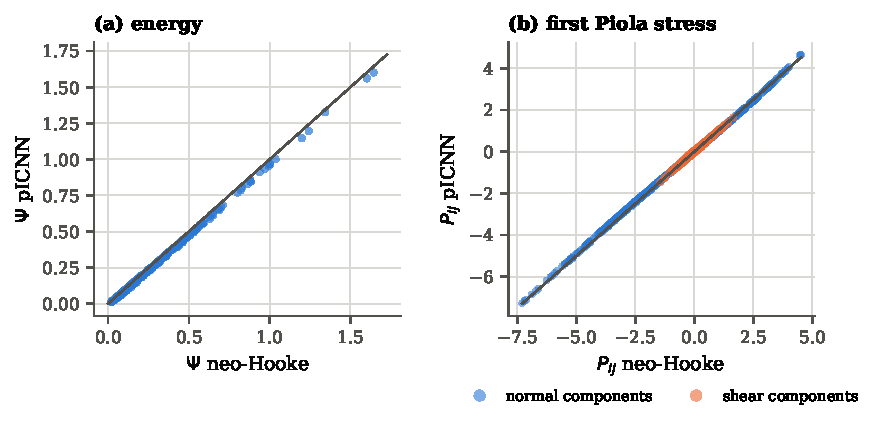
\includegraphics[width=0.9\textwidth]{fig_v2b.pdf}
\caption[V2b: Phase~1 network versus the neo-Hookean law]{V2b: Phase~1 network versus the analytical neo-Hookean law on 256 validation states. (a) Energy. (b) All components of the first Piola stress. Line: identity.}
\label{fig:v2b}
\end{figure}


\testcase{V3}{Automatic-differentiation tangent}
\taim Verify $\Aten=\partial\Pstress/\partial\F$ from AD against central
differences of $\Pstress$.
\tsetup Four seeded deformation gradients; $\epsilon=10^{-2},\dots,10^{-8}$.
Finite differences serve only as the check.
\trun \code{python -m tests.verify\_tangent}
\texpect A V-shaped error curve: truncation error $\propto\epsilon^2$ for large
$\epsilon$, round-off error $\propto\varepsilon_\mathrm{mach}/\epsilon$ for small
$\epsilon$; minimum below $10^{-6}$.
\tobtain \Cref{fig:v3}. The errors are $1.5\times10^{-5}$, $1.5\times10^{-9}$,
$2.3\times10^{-10}$ and $2.3\times10^{-8}$. The decrease by four decades per two
decades of $\epsilon$ confirms the $\epsilon^2$ truncation order. Pass.
\tinfer Automatic differentiation gives the exact tangent: the observed difference to central differences is entirely the truncation and round-off of the reference, with the expected $\epsilon^2$ slope. The finite-difference tangent of the original proposal could never match this accuracy.

\begin{figure}[H]
\centering
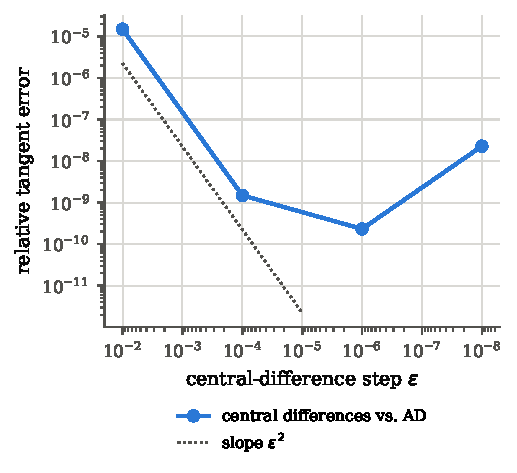
\includegraphics[width=0.5\textwidth]{fig_v3.pdf}
\caption[V3: central-difference error of the AD tangent]{V3: central-difference error of the AD tangent. It first decreases as $\epsilon^2$ (dotted guide) and then increases through round-off.}
\label{fig:v3}
\end{figure}


\testcase{V4}{Newton convergence of the nonlinear FE solve}
\taim Verify that the quadrature-point transfer and the consistent tangent
yield quadratic Newton convergence.
\tsetup Unit cube, $h=0.4$, $P_1$; $u_x=0.1x$ prescribed on $x=0$ and $x=1$;
trained Phase~1 network; tolerance $\|\bm R_\mathrm{free}\|<10^{-8}$.
\trun \code{python -m tests.verify\_element --ckpt checkpoints\slash{}phase1\_validated.pt}
\texpect $\|\bm R_{k+1}\|/\|\bm R_k\|^2$ bounded and the empirical order
\[q_k=\frac{\ln(r_{k+1}/r_k)}{\ln(r_k/r_{k-1})}\;\to\;2,\qquad r_k=\|\bm R_k\|.\]
\tobtain \Cref{tab:newton} and \cref{fig:v4}. Four iterations; the ratio stays
below 1 and $q$ rises to $1.90$. Quadratic convergence. Pass.
\tinfer The assembly, the quadrature-point transfer and the AD tangent are mutually consistent, because the Newton method converges with order close to two. A wrong tangent would reduce it to linear convergence.

\begin{figure}[H]
\centering
\begin{subfigure}[b]{0.42\textwidth}\centering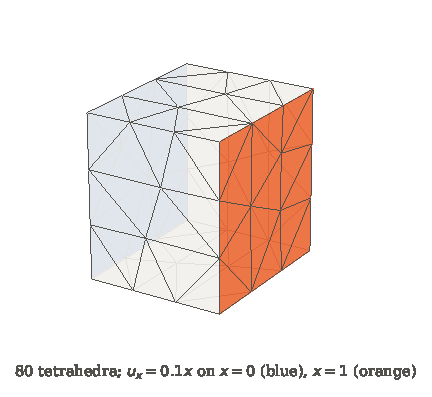
\includegraphics[width=\textwidth]{fig_v_setup_v4.pdf}\end{subfigure}\hfill
\begin{subfigure}[b]{0.55\textwidth}\centering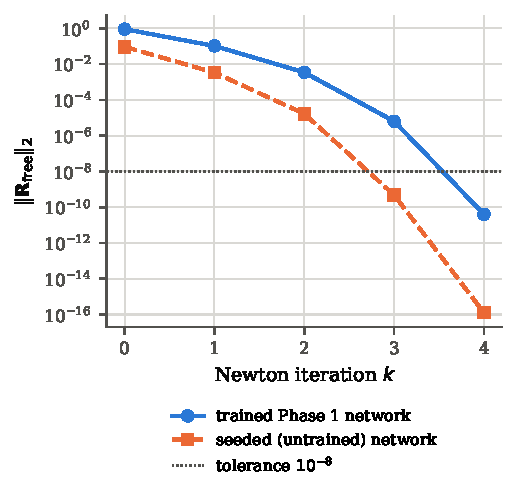
\includegraphics[width=\textwidth]{fig_v4.pdf}\end{subfigure}
\caption[V4: boundary-value problem and Newton residuals]{V4. (a) Boundary-value problem: unit cube, 80 tetrahedra, $u_x=0.1x$ on $x=0$ (blue, hidden) and $x=1$ (orange), lateral faces free. (b) Newton residuals of the trained and of an untrained (seeded) network.}
\label{fig:v4}
\end{figure}

\begin{table}[H]
\centering\small
\caption{V4: Newton residuals (tolerance $10^{-8}$).}
\label{tab:newton}
\begin{tabular}{@{}rccc@{}}
\toprule
$k$ & $\|\bm R_\mathrm{free}\|_2$ & $\|\bm R_{k+1}\|/\|\bm R_k\|^2$ & $q_k$\\
\midrule
0 & $9.058\times10^{-1}$ & 0.127 & --\\
1 & $1.043\times10^{-1}$ & 0.318 & 1.58\\
2 & $3.463\times10^{-3}$ & 0.535 & 1.85\\
3 & $6.412\times10^{-6}$ & 0.978 & 1.90\\
4 & $4.023\times10^{-11}$ & -- & --\\
\bottomrule
\end{tabular}
\end{table}

\testcase{V5}{Affine patch test}
\taim Verify that a homogeneous deformation is reproduced exactly on an
unstructured multi-element mesh through the full material path.
\tsetup Unit cube with 206 irregular tetrahedra (2884 material points). All boundary
nodes follow $\bm F_\mathrm{target}=\begin{bmatrix}1.08&0.05&0\\0&0.97&0.03\\0&0&1.02\end{bmatrix}$;
the interior nodes are free.
\begin{figure}[H]
\centering
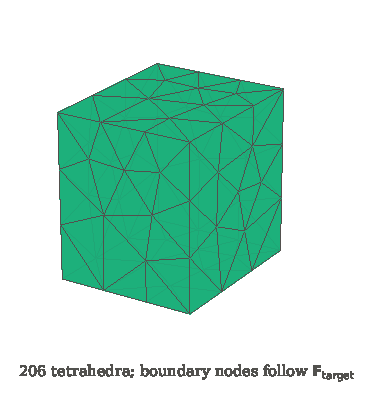
\includegraphics[width=0.33\textwidth]{fig_v_setup_v5.pdf}
\caption[V5: boundary-value problem]{Boundary-value problem of V5: unit cube with 206 tetrahedra; all boundary nodes follow $\bm F_\mathrm{target}$, interior nodes free.}
\label{fig:vsetup5}
\end{figure}

\trun \code{python -m tests.verify\_patch --ckpt checkpoints\slash{}phase1\_validated.pt}
\texpect Uniform $\F$ and $\Pstress$, and a vanishing free residual.
\tobtain $\max|\F-\bm F_\mathrm{target}|=4.4\times10^{-16}$, relative stress variation
$4.6\times10^{-15}$, $\|\bm R_\mathrm{free}\|=2.7\times10^{-16}$. Pass.
\tinfer The material path reproduces a homogeneous state exactly on an irregular mesh, so there is no spurious force from the transfer between the network and the finite-element space.

\testcase{V6}{Matched analytical and neural FE solutions}
\taim Compare complete nonlinear FE solutions obtained with the neural and the
analytical material.
\tsetup V4 geometry, $10\,\%$ stretch, lateral faces free; tolerance 15\,\% on
displacement, $\F$ and reaction vector.
\begin{figure}[H]
\centering
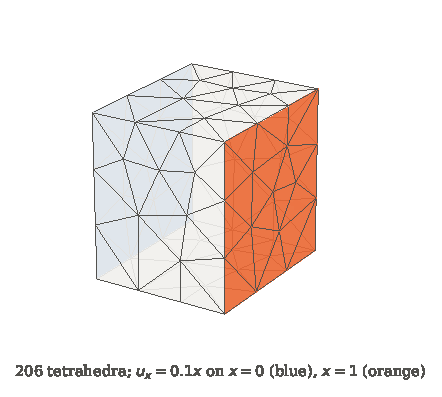
\includegraphics[width=0.33\textwidth]{fig_v_setup_v6.pdf}
\caption[V6: boundary-value problem]{Boundary-value problem of V6: unit cube with 206 tetrahedra, $u_x=0.1x$ on $x=0$ (blue, hidden) and $x=1$ (orange), lateral faces free.}
\label{fig:vsetup6}
\end{figure}

\trun \code{python -m tests.verify\_fe\_comparison --ckpt checkpoints\slash{}phase1\_validated.pt}
\tobtain Both solves converge in five iterations. The relative errors are
$2.00\,\%$ (displacement), $0.35\,\%$ ($\F$) and $13.4\,\%$ (reaction). Pass. The reaction error is close to its limit. Its origin is identified
by V8: the Phase~1 network has a small-strain shear modulus of $0.883$ instead of
$1$ ($-11.7\,\%$), although its relative stress error in V2b is only $3.3\,\%$.
\tinfer Network and analytical law give the same deformation field (displacement and $\F$ within $2\,\%$ and $0.4\,\%$); the larger reaction error is caused by the Phase~1 network's shear modulus and not by the bridge.

\testcase{V7}{Single element under full deformation control}
\taim Verify the constitutive response and the consistent tangent of one
element when every nodal degree of freedom is prescribed. Following the
guideline, the physically linear but geometrically nonlinear St.\ Venant--Kirchhoff
law, $\Psi=\tfrac{\lambda}{2}(\operatorname{tr}\bm E)^2+\mu\operatorname{tr}\bm E^2$, is
tested before the neo-Hookean law ($\mu=1$, $\lambda=10$).
\tsetup One trilinear hexahedron (unit cube, $2\times2\times2$ Gauss rule). All nodes
follow the affine map of the non-symmetric
$\Fbar=\begin{bmatrix}1.10&0.06&-0.02\\0.03&0.92&0.05\\-0.04&0.02&1.05\end{bmatrix}$.
The assembled stiffness $\bm K$ (production \code{assemble\_system}) is compared with
central differences of the assembled residual along a random direction.
\trun \code{python -m tests.verify\_stress\_control}
\texpect $\F=\Fbar$ and $\Pstress=\Pstress^{\mathrm{analytic}}(\Fbar)$ at every Gauss point to
round-off; tangent error $\propto\epsilon^2$ until round-off.
\tobtain $\max|\F-\Fbar|=2.4\times10^{-16}$; relative stress error $5.5\times10^{-15}$
(SVK) and $3.4\times10^{-15}$ (neo-Hooke). Tangent errors fall from $8.5\times10^{-6}$
($\epsilon=10^{-3}$) to $1.7\times10^{-11}$ ($\epsilon=10^{-6}$) for SVK, and from
$3.5\times10^{-6}$ to $1.8\times10^{-11}$ for neo-Hooke, decreasing by two decades per decade of $\epsilon$
(\cref{fig:v7}). Pass.
\tinfer The constitutive response and the assembled tangent are correct for a general, non-symmetric $\Fbar$ including the geometric nonlinearity; the tangent error is limited only by the difference step.

\begin{figure}[H]
\centering
\begin{subfigure}[b]{0.42\textwidth}\centering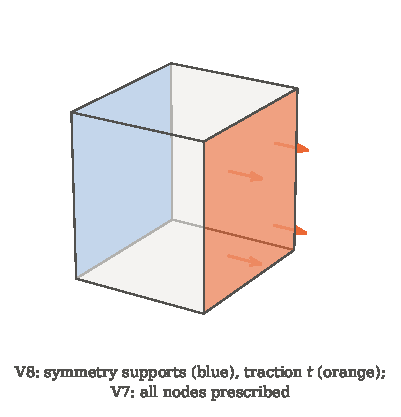
\includegraphics[width=\textwidth]{fig_v_setup_v78.pdf}\end{subfigure}\hfill
\begin{subfigure}[b]{0.55\textwidth}\centering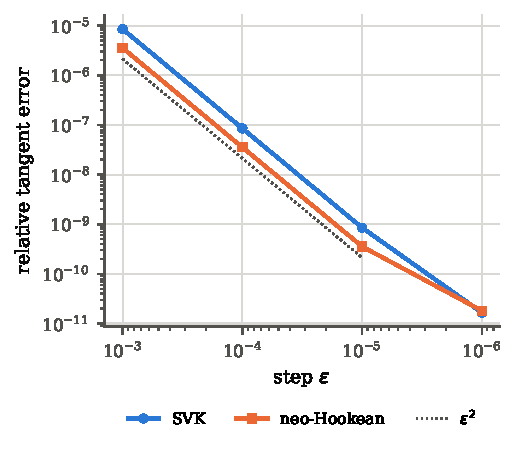
\includegraphics[width=\textwidth]{fig_v7.pdf}\end{subfigure}
\caption[V7/V8: boundary-value problems and V7 tangent error]{V7 and V8. (a) Boundary-value problems of the single trilinear hexahedron. V7: all nodes prescribed by the affine map. V8: symmetry supports on $x=0$, $y=0$, $z=0$ (blue) and nominal traction $t$ on $x=1$ (orange). (b) V7: error of the assembled tangent against central differences of the residual (SVK and neo-Hooke); dotted: slope $\epsilon^2$.}
\label{fig:v7}
\end{figure}


\testcase{V8}{Single element under stress control}
\taim Verify the solver under prescribed tractions (Neumann boundary
conditions) with only the minimal supports, including quadratic Newton
convergence in every load step.
\tsetup The same hexahedron with symmetry supports $u_x=0$ on $x=0$, $u_y=0$ on $y=0$
and $u_z=0$ on $z=0$; dead-load nominal traction $(t,0,0)$ on $x=1$, increased to
$t=0.6$ in three steps; all other faces free. The reference solution
$\F=\operatorname{diag}(a,b,b)$ is computed independently from $P_{11}=t$,
$P_{22}=P_{33}=0$. Tractions and component-wise supports are options of the production solver \code{solve}.
\trun \code{python -m tests.verify\_stress\_control --ckpt checkpoints/phase1\_validated.pt}
\texpect Homogeneous FE solution with $F_{11}=a$, $F_{22}=F_{33}=b$ and
$\Pstress=\operatorname{diag}(t,0,0)$ to round-off; quadratic Newton convergence.
\tobtain \Cref{tab:v8} and \cref{fig:v8}. For both analytical laws the stretches agree with the
reference to $\le2.4\times10^{-15}$ and $|\Pstress-\operatorname{diag}(t,0,0)|/t\le1.4\times10^{-14}$;
each load step converges in four Newton iterations with an empirical order of about
2 (for example $10^{-1}\to3.7\times10^{-2}\to1.4\times10^{-4}\to2.6\times10^{-8}\to7.8\times10^{-16}$
for neo-Hooke at $t=0.6$). Pass. The trained Phase~1 network, run through the same
test for comparison, satisfies equilibrium ($|\Pstress-\operatorname{diag}(t,0,0)|/t=10^{-12}$),
but its stretches deviate from neo-Hooke by $+17.8\,\%$ of the axial stretch increment at
$t=0.2$ and by $+31\,\%$ at $t=0.6$, where $a=1.25$ also exceeds the Phase~1 training
range. The cause is its shear modulus of $0.883$, a constitutive (not a solver) error.
\tinfer The solver handles prescribed tractions with minimal supports and converges quadratically in every step. The deviation of the Phase~1 network from the neo-Hookean law is a property of the network, which confirms the shear-modulus defect found in V6.

\begin{figure}[H]
\centering
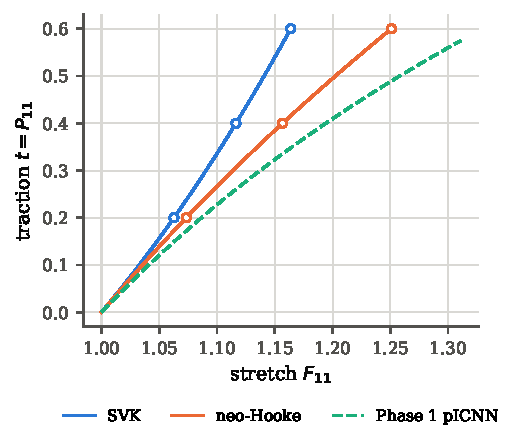
\includegraphics[width=0.5\textwidth]{fig_v8.pdf}
\caption[V8: uniaxial nominal traction versus axial stretch]{V8: uniaxial nominal traction versus axial stretch. Lines: independent reference solution of $P_{11}=t$, $P_{22}=P_{33}=0$; circles: FE solution after each load step (agreement to $\le2.4\times10^{-15}$). The Phase~1 network is softer than the neo-Hookean law it was trained on.}
\label{fig:v8}
\end{figure}

\begin{table}[H]
\centering\small
\caption{V8: uniaxial stress control of one hexahedron at $t=0.6$.}
\label{tab:v8}
\setlength{\tabcolsep}{4pt}
\begin{tabular}{@{}lcccc@{}}
\toprule
Material & reference $a$ / $b$ & $\max|F_{11}-a|$ & $\max|F_{22,33}-b|$ & it./step\\
\midrule
St.\ Venant--Kirchhoff & 1.1638045 / 0.9159096 & $1.3\times10^{-15}$ & $1.6\times10^{-15}$ & 4\\
neo-Hooke & 1.2509757 / 0.9024160 & $2.4\times10^{-15}$ & $1.9\times10^{-15}$ & 4\\
Phase~1 pICNN & as neo-Hooke & $7.9\times10^{-2}$ & $5.3\times10^{-2}$ & 4\\
\bottomrule
\end{tabular}
\end{table}

% ======================================================================
\section{Phase 2: periodic RVE and homogenization}

The tests run on reduced meshes ($h=0.22$--$0.35$). Each prints its metrics and a
PASS line.

\testcase{P2-V1}{Periodic space}
\taim Opposite faces must carry identical fluctuation values.
\tsetup Periodic $P_2$ space on the cell with cavity (371 elements).
\trun \code{python -m tests.verify\_periodic\_rve}
\tobtain 2208 unconstrained active DOFs are reduced to 1485 (723 eliminated). The
maximum opposite-face jump is $2.2\times10^{-16}$. Pass.
\tinfer The periodic space is exactly triply periodic, so no spurious boundary stress enters the RVE solution.

\testcase{P2-V2}{Rigid kinematics}
\taim The prescribed cavity trace must be an exact rigid motion: six independent
modes, and proper rotations at finite angles.
\trun \code{python -m tests.verify\_rigid\_particle}
\tobtain Distance error $1.1\times10^{-16}$; rigid-map rank 6; constraint residual
$7.2\times10^{-18}$; linearization error of the rotation increment
$7.7\times10^{-10}$. Pass.
\tinfer The rigid particle is exactly rigid and its rotation is a proper rotation, so the penalty parameter of the proposal is no longer needed.

\testcase{P2-V3}{Mixed patch at $\kappa/\mu=10^4$}
\taim The Taylor--Hood formulation must reproduce a homogeneous finite deformation
exactly, without volumetric locking.
\trun \code{python -m tests.verify\_mixed\_matrix}
\tobtain Errors in $\F$, $J$ and $p$ of $2.3\times10^{-15}$, $2.2\times10^{-15}$ and
$2.9\times10^{-13}$; pressure variation $3.6\times10^{-15}$; final residual
$6.3\times10^{-16}$. Pass.
\tinfer The Taylor--Hood pair is free of volumetric locking at $\kappa/\mu=10^4$, which is what allows the RVE to represent the near-incompressible matrix.

\testcase{P2-V4}{Coupled periodic RVE}
\taim The periodic matrix and the rigid particle must be in equilibrium together.
\trun \code{python -m tests.verify\_coupled\_rve}
\tobtain Rigid-trace error $8.0\times10^{-19}$; relative particle force and moment
$2.1\times10^{-7}$ and $7.4\times10^{-9}$ (prescribed rotation); final residual
$1.9\times10^{-14}$. Pass.
\tinfer Matrix and particle are in equilibrium, and the periodic jump and the rigid trace are exact to round-off; the particle force and moment are small but not machine zero because the rotation is prescribed in this test.

\testcase{P2-V5}{Hill--Mandel macro-homogeneity}
\taim The homogenized stress \cref{eq:hm} must be work-conjugate to $\Fbar$.
\tsetup Finite hydrostatic loading of the cell; mixed $P_2/P_1$, $\kappa/\mu=10^4$.
Macroscopic and microscopic virtual powers are compared for independent virtual
rates. A constant-stress recovery checks sign, index order and volume
normalization.
\trun \code{python -m tests.verify\_hill\_mandel}
\texpect Equal powers to round-off.
\tobtain Microscopic and macroscopic power are both $470.9456611477$; relative error
$1.2\times10^{-15}$; alternative virtual field $1.4\times10^{-15}$; constant-stress
recovery $4.0\times10^{-14}$. The raw boundary-traction estimate, kept as a
diagnostic, is off by $3.9\times10^{-6}$. This confirms that the reaction term in
\cref{eq:hm} is necessary. Pass.
\tinfer The reaction-based homogenized stress satisfies the Hill--Mandel condition, whereas the naive boundary-traction estimate is wrong at the $10^{-6}$ level; the reaction term is therefore required.

\testcase{P2-V6}{Condensed homogenized tangent}
\taim Verify \cref{eq:schur}: major symmetry, consistency with the stress, and
second-order Taylor remainder.
\tsetup Cell with prescribed particle rotation (1472 elements), loaded off the
identity. Remainder $r(t)=\|\Pbar(\Fbar+t\bm D)-\Pbar(\Fbar)-t\Abar:\bm D\|$ for
$t=10^{-3},5\times10^{-4},2.5\times10^{-4}$, re-solving the RVE at each step.
\trun \code{python -m tests.verify\_homogenized\_tangent}
\texpect $r\propto t^2$, that is, observed order 2.
\tobtain (\cref{fig:vp2v6}) $r=6.760\times10^{-3}$, $1.690\times10^{-3}$, $4.225\times10^{-4}$, giving
orders $2.000$ and $2.000$. Symmetry error $3.0\times10^{-16}$; energy-gradient
stress error $6.7\times10^{-16}$; independent sensitivity error
$1.7\times10^{-15}$. Pass.
\tinfer The condensed tangent is exact: it is the derivative of the stress, it is symmetric, and the second-order Taylor remainder shows that no first-order error is present.

\begin{figure}[H]
\centering
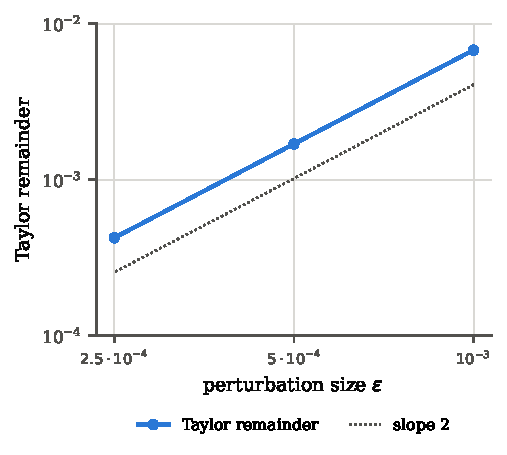
\includegraphics[width=0.5\textwidth]{fig_v_p2v6.pdf}
\caption[P2-V6: Taylor remainder of the condensed RVE tangent]{P2-V6: Taylor remainder of the condensed RVE tangent versus perturbation size; dotted: slope 2.}
\label{fig:vp2v6}
\end{figure}


\testcase{P2-V7}{Free finite particle rotation}
\taim Under simple shear ($\gamma=0.05$) the free particle must rotate until its
resultant moment vanishes, while $\Rten$ stays a proper rotation.
\trun \code{python -m tests.verify\_free\_rotation}
\tobtain Three outer Newton iterations reduce the moment residual from
$4.75\times10^{-3}$ to $8.0\times10^{-16}$. The particle rotates by
$-0.0249\,$rad about $z$. Orthogonality error $2.5\times10^{-16}$; determinant error
$4.4\times10^{-16}$; rotational-Hessian symmetry $1.3\times10^{-17}$. Pass.
\tinfer The free rotation is determined by moment equilibrium within three outer iterations, with proper orthogonality, so the particle can be treated as freely rotating at no extra modelling error.

\testcase{P2-V8}{Translation gauge}
\taim A common translation of the fluctuation and the particle must leave all
physical fields unchanged.
\trun \code{python -m tests.verify\_translation\_gauge}
\tobtain For a shift of $2.7\times10^{-3}$, the changes in $\F$, $p$, pointwise stress and
homogenized stress are $1.1\times10^{-15}$, $4.0\times10^{-15}$, $8.9\times10^{-15}$ and
$1.2\times10^{-15}$. Pass.
\tinfer The translation of the particle is a pure gauge, which justifies fixing it without changing any physical result.

\testcase{P2-V9}{Free-rotation homogenized tangent against re-solved central differences}\label{sec:p2v9}
\taim Verify the complete production tangent of the freely rotating particle,
including rotational condensation, against the strongest possible reference:
central differences in which the full nonlinear RVE, including the rotation
equilibrium, is \emph{re-solved} at every perturbed macroscopic state.
\tsetup Pilot record \code{v001\_f000047} ($\vfrac=0.05$, $J_{\min}=0.65$ and
$J_{\max}=1.59$ inside the cell), production settings ($h=0.22$, $P_2/P_1$,
integration order 10). Step $10^{-4}$ in all nine row-major directions of $\Fbar$, that
is $1+18$ full RVE solves, plus objectivity re-solves under rotated $\Fbar$.
\trun \code{python -m benchmarks.rve\_constitutive\_checks --dataset <pilot.npz> --output p2v9.json --sample-ids v001\_f000047}
\texpect Agreement within the stored tolerances: tangent $5\times10^{-3}$, energy gradient
$5\times10^{-4}$, stress $5\times10^{-5}$, objectivity $10^{-6}$ (energy).
\tobtain Status \emph{pass}, after $59.6\,$min on one core. The maximum
directional tangent error is $5.2\times10^{-12}$ and the maximum energy-gradient
error $1.8\times10^{-11}$. Base-stress work versus condensed stress agrees to
$7.6\times10^{-16}$; objectivity errors are $1.3\times10^{-15}$ (energy) and
$1.2\times10^{-15}$ (stress). The equilibrium residuals are $1.3\times10^{-13}$
(mixed), $6.5\times10^{-15}$ (rotation) and $6.2\times10^{-13}$ (condensed). The free-rotation tangent is
therefore exact to the accuracy of the re-solved differences.
\tinfer The full free-rotation tangent, including the condensation of the rotation, agrees with finite differences of re-solved RVEs to the accuracy of the differences; it is therefore exact and can be used by a Newton solver.


\testcase{P2-V10}{Dataset contract}
\taim Generation must be deterministic and splits must be leak-free.
\trun \code{python -m tests.verify\_rve\_dataset}
\tobtain 12 states at two volume fractions; regeneration error $0$; zero cross-split
leaks; a different seed changes the states (by $0.28$); serialization error $0$;
tangent shape $(9,9)$. Pass.
\tinfer Datasets are reproducible and the splits do not leak, so the test statistics of \cref{ch:assessment} are not contaminated by overlapping states.

% ======================================================================
\paragraph{Newton convergence across all solvers.} \Cref{fig:vnewton} collects the
residual histories of every nonlinear solve in the test suite: the Phase~1 bridge
(V4, V6), the single hexahedron under stress control (V8), the mixed patch
(P2-V3), the coupled RVE (P2-V4), the outer rotation iteration (P2-V7) and the
first load increment of the macroscopic problem (M-V0). All show the
characteristic quadratic tail, with the number of correct digits roughly doubling
in each of the last iterations. Since each solver uses its own exact or AD
Jacobian, this is a joint check of all tangents in the code. \Cref{fig:vrvechecks}
summarizes the identities checked by the RVE tests.

\begin{figure}[H]
\centering
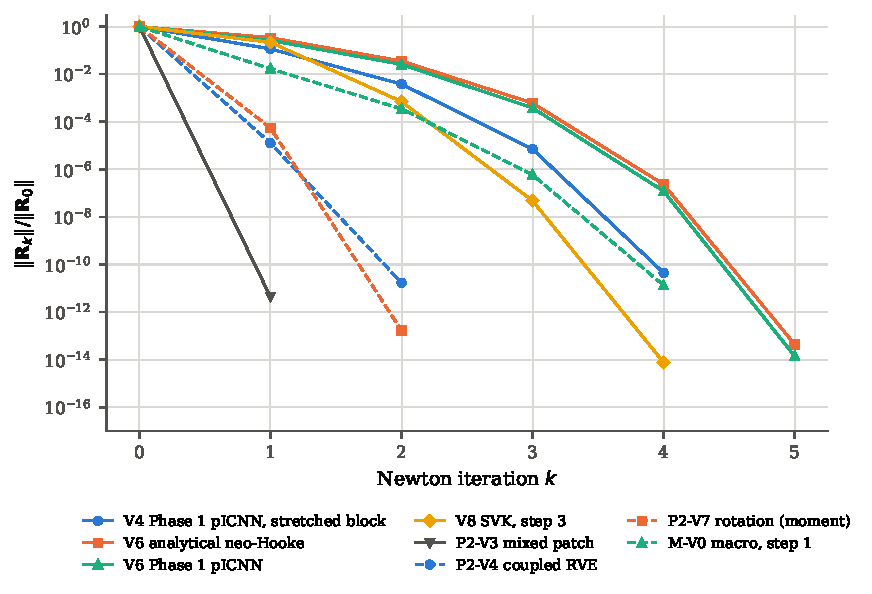
\includegraphics[width=0.95\textwidth]{fig_v_newton_all.pdf}
\caption[Normalized Newton residuals of all nonlinear solves]{Normalized Newton residuals of all nonlinear solves in the test suite. P2-V3 ($J=1.001$) converges in one step.}
\label{fig:vnewton}
\end{figure}

\begin{figure}[H]
\centering
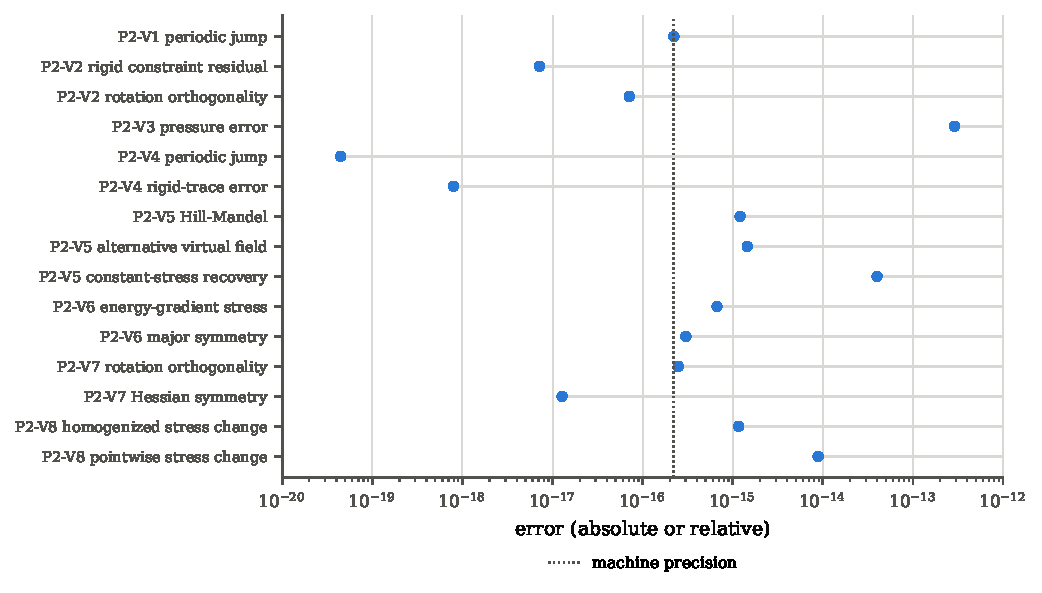
\includegraphics[width=0.95\textwidth]{fig_v_rve_checks.pdf}
\caption[Identities checked by the RVE tests P2-V1 to P2-V8]{Identities checked by the RVE tests P2-V1 to P2-V8 (absolute or relative errors as printed by the tests); dotted: machine precision.}
\label{fig:vrvechecks}
\end{figure}

\section{Surrogate and macroscopic tangent checks}

\testcase{S-V1}{Constitutive consistency of the trained surrogate}
\taim For an RVE-trained checkpoint, check on held-out states that
$\partial\widehat\Psi/\partial\F$ equals the returned stress and that the
tangent equals directional differences of the stress, and check objectivity
($\widehat\Psi(\bm Q\F)=\widehat\Psi(\F)$) and major symmetry.
\tsetup 36 records (12 states, three volume fractions), central differences with
step $10^{-5}$, thresholds $10^{-6}$ (gradient), $10^{-5}$ (tangent), $10^{-10}$
(objectivity).
\trun \code{python -m benchmarks.rve\_surrogate\_constitutive\_checks --dataset <phase7.npz> ...} (\cref{ch:manual})
\tobtain Frozen checkpoint: status \emph{pass} for 36 records (\cref{fig:vs1});
energy gradient $4.9\times10^{-8}$, tangent $1.0\times10^{-9}$, objectivity
$4.8\times10^{-13}$ (energy) and $1.7\times10^{-12}$ (stress), symmetry $6.0\times10^{-16}$.
During development the same test \emph{failed} for the Phase~5
checkpoint (objectivity energy error $0.91$), which led to the objective correction
\cref{eq:norm}. The test thus detected a physical defect that an accuracy metric
could not reveal.
\tinfer Stress and tangent of the surrogate are exact derivatives of its energy, and the energy is objective and symmetric on held-out states. The surrogate is thus a valid hyperelastic law; its remaining deficit (\cref{ch:assessment}) is accuracy, not consistency.

\begin{figure}[H]
\centering
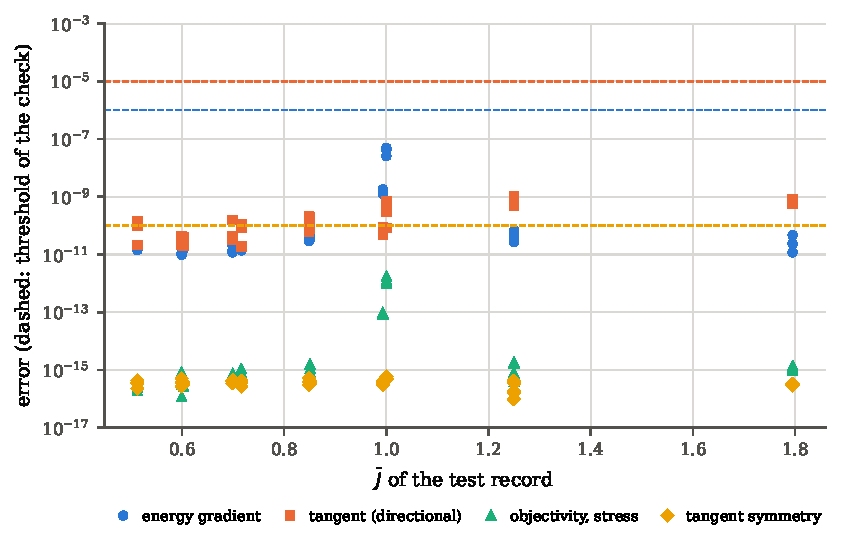
\includegraphics[width=0.95\textwidth]{fig_v_s1.pdf}
\caption[S-V1: errors of the frozen surrogate for the audited records]{S-V1: errors of the frozen surrogate for the 36 audited test records versus $\overline J$; dashed lines: thresholds of the corresponding checks (same colour).}
\label{fig:vs1}
\end{figure}


\testcase{M-V0}{Macroscopic tangent consistency}
\taim Verify the assembled global stiffness of the macro problem against
directional differences of the residual at a non-equilibrium iterate.
\trun \code{python -m benchmarks.phase6\_macro\_fe\_demo --tangent-check-only ...}; full command in \code{tests/README.md}
\tobtain Frozen checkpoint ($P_1$, $h=0.25$, predictor state of the
second increment at $1\,\%$ stretch): relative directional error $6.5\times10^{-10}$;
symmetry error $1.5\times10^{-16}$; Newton linear solve accurate to $5.1\times10^{-16}$.
The free stiffness has eigenvalues of magnitude $0.44$ to $1.46\times10^4$, a condition
estimate of $3.3\times10^4$, of the order of $\kappa/\mu=10^4$, and one negative eigenvalue at this
non-equilibrium predictor state. This is the conditioning that governs the
macroscopic solver behaviour discussed in \cref{sec:macro}.
\tinfer The assembled macroscopic tangent is consistent with the residual, so any slow macroscopic convergence stems from the conditioning and the nonlinear path, not from a faulty Jacobian.

\chapter{Surrogate Assessment and Macroscopic Application}\label{ch:assessment}

This chapter evaluates whether the trained surrogate reproduces the direct RVE
solutions and whether it can be used in a macroscopic simulation. After the
comparison with the proposal and the committee's recommendations, the RVE is checked
against micromechanics, the training and test performance of the surrogate are
presented, and its errors are analysed separately for volumetric and deviatoric
response.

\section{Proposal goals and their achievement}

{\small
\begin{xltabular}{\textwidth}{@{}p{3.6cm}p{2.3cm}X@{}}
\caption{Milestones of the proposal and their outcome.}\label{tab:proposal}\\
\toprule
Proposal item & Status & Outcome / justification\\
\midrule
\endfirsthead
\caption[]{\emph{(continued)}}\\
\toprule
Proposal item & Status & Outcome / justification\\
\midrule
\endhead
\bottomrule
\endfoot
M1 Environment, repository, periodic RVE, kinematic check (target $<10^{-12}$) &
  achieved & Native periodic spaces; P2-V1 jump $2.2\times10^{-16}$.\\
M2 Hill--Mandel averaging, data over $\vfrac$ (target: energy deviation $<1\,\%$) &
  achieved, exceeded & Reaction-based stress; P2-V5 $1.2\times10^{-15}$; ten datasets with 4653 distinct direct-RVE records.\\
Rigid glass via stiffness penalty & replaced & Exact rigid trace with free rotation (no penalty parameter, no particle deformation).\\
RVE tangent by forward differences & replaced & Exact Schur condensation, Taylor order $2.000$ (P2-V6); differences used only for checks.\\
M3 pICNN, softplus weights, normalization, Sobolev loss & implemented; accuracy \emph{not} achieved in shear &
  Polyconvex architecture verified (S-V1); normalization corrected to an objective form; deviatoric accuracy is limited by loss scaling (\cref{sec:diagnosis}).\\
pICNN inputs $\mathcal N(I_1,I_2,\vfrac)$ & extended & Features $[I_1,I_2,J,-\ln J]$ plus $\vfrac$ context; $J$ is needed for the compressible volumetric response and the stress-free normalization.\\
Sobolev loss with $\lambda_A\gg\lambda_\Psi$ (tangent prioritized) & \emph{not} followed &
  Implemented weights $w_\Psi=1$, $w_P=1$, $w_A=0.1$ on a relative-Frobenius tangent term (\cref{eq:loss}); the tangent was not prioritized, and its relative norm is itself volumetric-dominated (\cref{sec:diagnosis}).\\
V3: FD error ``drops to machine precision at $\epsilon\to10^{-7}$'' & corrected expectation &
  Not attainable: V3 shows the truncation/round-off V-curve with minimum $2.3\times10^{-10}$ near $\epsilon=10^{-6}$; FD is used only as a check.\\
V4 on a single hexahedral element & changed &
  V4 uses a coarse tetrahedral cube mesh; single-hexahedron tests are V0d/V0e, V7 and V8.\\
Material data $\mu_\mathrm{PDMS}\approx2\,$MPa, $E_\mathrm{glass}\approx70\,$GPa & idealized &
  Dimensionless $\mu=1$, $\kappa=10^4$; glass exactly rigid (no $E_\mathrm{glass}$ needed); no calibration to measured PDMS.\\
M1 continuous-integration pipeline & achieved &
  GitHub Actions workflow and the runner \code{run\_tests.sh}, in addition to manual and PBS test runs.\\
AI tools ``strictly'' for syntax, plotting templates, NumPy & broader use &
  Also used for understanding theory and libraries, discussing code structure and
  errors, test cases, PBS scripts and writing support (\cref{ch:chatbots}).\\
M4 AD tangent, $6\times6$ Voigt mapping, FD check & achieved, corrected & Full $9\times9$ tangent instead of $6\times6$; V3 minimum error $2.3\times10^{-10}$.\\
M5 Macroscopic BVP, custom Newton, manual assembly & achieved & Bridge with globalized Newton; macro tangent check $6.5\times10^{-10}$ (M-V0).\\
M6 Single-element benchmark (quadratic convergence) and multi-element component (dogbone) &
  partly achieved & V4 quadratic; clamped-cube component instead of a dogbone; $P_1$ reaches $5\,\%$ but is locked; $P_2$ reaches $1\,\%$ on two of three meshes (\cref{sec:macro}).\\
M7 Documentation, README per test, defense & achieved & Manual in \cref{ch:manual}; \code{tests\slash{}README.md} lists command, inputs and expected result of every test.\\
\end{xltabular}
}

\paragraph{Additional work beyond the proposal.} The following studies were not
promised and were carried out in addition, all with the frozen checkpoint: the
30-case timing benchmark (\cref{ch:performance}), the loading-path sweep, the
volume-fraction map, inverse design of $\vfrac$, the cell-orientation (isotropy)
audit, the small-strain micromechanics comparison, and the sampled acoustic-tensor
screen. The shear-adaptation study belongs to the main scope as a corrective step.

\section{Response to the committee's recommendations}\label{sec:committee}

After the proposal defense, the committee (Dr.\ S.\ Pr\"uger) asked first for a
proof of concept of the pICNN, including stress and tangent, inside NGSolve, and
only then for RVE data generation. It also raised several technical questions.
\Cref{tab:committee} lists each point and where the report answers it.

{\small
\begin{xltabular}{\textwidth}{@{}p{5.0cm}X@{}}
\caption{Committee recommendations and their implementation.}\label{tab:committee}\\
\toprule
Recommendation / question & Response in this project\\
\midrule
\endfirsthead
\caption[]{\emph{(continued)}}\\
\toprule
Recommendation / question & Response in this project\\
\midrule
\endhead
\bottomrule
\endfoot
Proof of concept first: pICNN with stress and tangent in NGSolve, trained on neo-Hookean data, before extensive data generation; establish with PyTorch what the TensorFlow tutorial shows &
  Phase~1 (\cref{sec:bridge}). The network is trained on the neo-Hookean law; the data
  are homogeneous states, so a single element under affine displacement reproduces
  them exactly. It is coupled through quadrature-point spaces to an NGSolve Newton
  solver and verified by V1--V6 and V0d before any RVE campaign.
  The TensorFlow tutorial and the closer NGSolve forum example are compared in
  \cref{tab:available}.\\
How are rigid inclusions handled? &
  No stiff phase: the cavity surface carries the exact rigid map \cref{eq:rigid};
  the rotation follows from moment equilibrium (P2-V2, P2-V7).\\
Periodicity through periodic function spaces on a periodic mesh &
  Implemented with Netgen face identification and NGSolve \code{Periodic} spaces;
  the custom ``PBC enforcer'' of the proposal was dropped (P2-V1).\\
How is the overall tangent computed? &
  Exact Schur condensation of the energy Hessian \cref{eq:schur}; Taylor order
  $2.000$ (P2-V6).\\
Macroscopic weak form: which fields, FE$^2$, or a mixed formulation for incompressibility? &
  Offline homogenization, not FE$^2$; the macro problem has displacements only. The
  locking analysis (\cref{sec:macro}) confirms the committee's concern: a mixed
  $u$--$p$ macro formulation is required for meaningful component responses.\\
The macro BVP is not ``driven by PyTorch'' &
  Wording corrected: NGSolve applies the boundary conditions and solves for the
  displacement; PyTorch only evaluates the constitutive law (\cref{sec:macro-method}).\\
Volumetric locking depends on the element choice &
  RVE: Taylor--Hood $P_2/P_1$ mixed formulation (P2-V3). Macro scale: locking of
  $P_1$ demonstrated quantitatively (\cref{tab:macro}).\\
Finite-difference tangent: choice of $\epsilon$ and attainable accuracy &
  FD is no longer used for any production tangent. V3 shows the expected
  truncation/round-off V-curve with a minimum error of $2.3\times10^{-10}$ near
  $\epsilon=10^{-6}$, so machine precision is \emph{not} reached by FD.\\
\end{xltabular}
}

\section{Physical plausibility of the RVE: small-strain moduli}

Before any surrogate is judged, its reference must be credible. Projecting the
direct-RVE tangent at $\Fbar=\Iten$ onto one volumetric and five orthonormal
deviatoric modes gives $K_{\mathrm{eff}}$ and $\mu_{\mathrm{eff}}$
(\cref{tab:moduli}, \cref{fig:moduli}). They lie within $0.2$--$1.1\,\%$ (bulk) and
$0.25$--$0.83\,\%$ (shear) of the Mori--Tanaka estimate \cref{eq:mt}, slightly
below it. The deviatoric anisotropy of the cubic cell grows from $0.2\,\%$ to
$4.1\,\%$ with $\vfrac$. This is the expected signature of one particle per cubic
cell, and it explains why the small deficit is not a bound violation. Rotating the
cell by three non-cubic rotations changed the energy and stress by at most
$5.6\times10^{-5}$ and $2.8\times10^{-5}$ (relative), which supports the isotropy
assumption of the surrogate within the tested states. The direct RVE is
therefore a sound reference.

\begin{table}[htbp]
\centering\small
\caption[Small-strain moduli ($\mu=1$, $\kappa=10^4$)]{Small-strain moduli ($\mu=1$, $\kappa=10^4$). The pICNN values of both checkpoints are computed directly from the network Hessian at $\F=\Iten$.}
\label{tab:moduli}
\begin{tabular}{@{}lccccccc@{}}
\toprule
& \multicolumn{3}{c}{$\mu_{\mathrm{eff}}$} & & \multicolumn{3}{c}{$K_{\mathrm{eff}}/10^4$}\\
\cmidrule{2-4}\cmidrule{6-8}
$\vfrac$ & 0.02 & 0.05 & 0.10 && 0.02 & 0.05 & 0.10\\
\midrule
Mori--Tanaka & 1.051 & 1.132 & 1.278 && 1.0204 & 1.0526 & 1.1111\\
direct RVE & 1.048 & 1.124 & 1.267 && 1.0185 & 1.0469 & 1.0988\\
pICNN frozen & 1.526 & 1.731 & 2.147 && 1.0231 & 1.0361 & 1.0873\\
pICNN shear-adapted & 1.349 & 1.527 & 1.892 && 1.0167 & 1.0478 & 1.0941\\
\midrule
frozen vs.\ RVE & $+45.6\,\%$ & $+54.0\,\%$ & $+69.5\,\%$ && $+0.4\,\%$ & $-1.0\,\%$ & $-1.0\,\%$\\
\bottomrule
\end{tabular}
\end{table}

\begin{figure}[htbp]
\centering
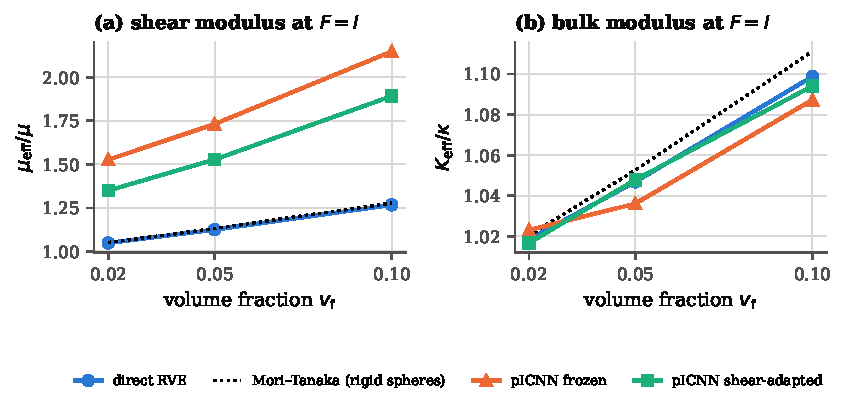
\includegraphics[width=\textwidth]{fig_small_strain_moduli.pdf}
\caption[Effective moduli at $\F=\Iten$]{Effective moduli at $\F=\Iten$. The direct RVE follows the Mori--Tanaka
estimate. Both surrogates reproduce the bulk modulus but overestimate the shear
modulus, by $46$--$70\,\%$ (frozen) and $29$--$49\,\%$ (shear-adapted).}
\label{fig:moduli}
\end{figure}

\paragraph{Inference.} The direct RVE is a credible reference: it reproduces the bulk and shear moduli of a rigid-sphere
composite to better than $1.2\,\%$ and is slightly softer than the Mori--Tanaka estimate, as expected
for a cubic arrangement. The surrogate inherits the correct bulk response but not the shear
response, so the shear error found later is a property of the surrogate, not of its labels.

\section{Training and test performance}\label{sec:trainperf}

\Cref{fig:training} shows the loss histories. The Phase~1 network trained on
neo-Hookean data decreases the loss by three orders of magnitude
(\cref{fig:training}a). On the RVE data, training and validation losses decrease
together by five orders of magnitude in the first stage (\cref{fig:training}b), and
continue to decrease slowly during the fine-tune on the combined Phase~6/7 data
(\cref{fig:training}c). Validation and training losses remain close throughout, so
there is no sign of overfitting; the oscillations reflect the small batch size and the
stochastic tangent sub-batch. The checkpoint with the lowest validation loss
(epoch~2750) was frozen.

\begin{figure}[htbp]
\centering
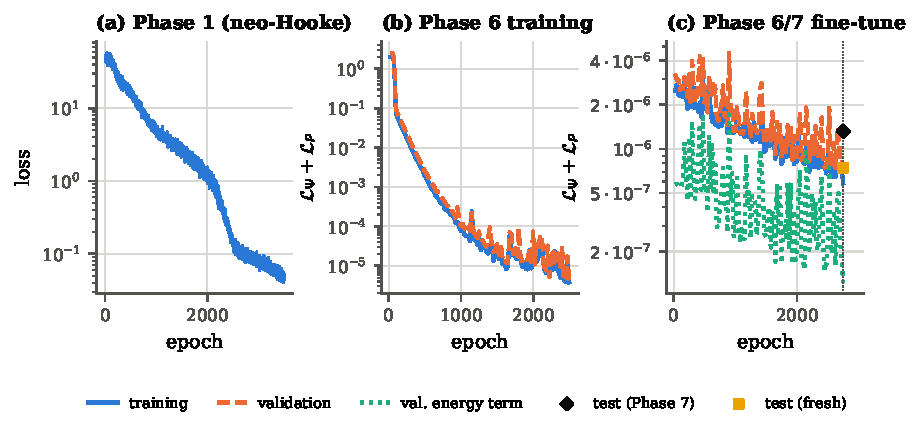
\includegraphics[width=\textwidth]{fig_training_curves.pdf}
\caption[Training histories]{Training histories. (a) Phase~1 network on neo-Hookean data. (b) First
training stage on the Phase~6 RVE data. (c) Fine-tune on Phase~6/7 data, with the
selected epoch (dotted line) and the losses of the frozen checkpoint on the two test
sets. Loss: energy and stress terms of \cref{eq:loss}, in normalized units.}
\label{fig:training}
\end{figure}

\Cref{tab:testloss} compares the losses of the frozen checkpoint on the training,
validation and test data. The test sets were not used for the gradient updates or the epoch selection of the stage in
which they are evaluated, but they are not all independent: the Phase~7 test split was
also evaluated with the stage-1 checkpoint, and 66 of the 600 Phase~7 records entered the
stage-2 training and validation sets. Only the fresh holdout of 90 records, generated after
the checkpoint was frozen, is fully independent.
The Phase~7 test split (531 states) and a fresh holdout of newly generated RVE
states (72 states) give energy-plus-stress losses of the same order as the training
loss ($1.3\times10^{-6}$ and $7.5\times10^{-7}$ against $5.8\times10^{-7}$). The model
therefore generalizes to unseen deformation states within the training envelope.

\begin{table}[htbp]
\centering\small
\caption[Losses of the frozen checkpoint]{Losses of the frozen checkpoint (normalized units of \cref{eq:loss}). Tangent:
mean squared relative Frobenius error of $\Aten$.}
\label{tab:testloss}
\begin{tabular}{@{}lrrrr@{}}
\toprule
Data set & States & $\mathcal L_\Psi$ & $\mathcal L_P$ & tangent\\
\midrule
training (selected epoch 2750) & -- & \multicolumn{2}{r}{$5.82\times10^{-7}$ (sum)} & --\\
validation & -- & $1.23\times10^{-7}$ & $5.27\times10^{-7}$ & --\\
test, Phase~7 split & 531 & $2.84\times10^{-7}$ & $1.03\times10^{-6}$ & $3.06\times10^{-5}$\\
test, fresh RVE holdout & 72 & $1.09\times10^{-7}$ & $6.37\times10^{-7}$ & $6.90\times10^{-5}$\\
\bottomrule
\end{tabular}
\end{table}

\Cref{fig:parity} shows parity plots of the Phase~7 test states, split into energy,
pressure and deviatoric stress. Energy and pressure lie on the diagonal over four
orders of magnitude, with median relative errors of $0.02\,\%$ and $0.025\,\%$. The
deviatoric stress scatters widely about the diagonal: the median error of its norm is
$82\,\%$ (the tensor error of \cref{tab:split} is $83\,\%$). The
small loss values in \cref{tab:testloss} therefore do not imply an accurate shear
response; the next two sections quantify and explain this.

\begin{figure}[htbp]
\centering
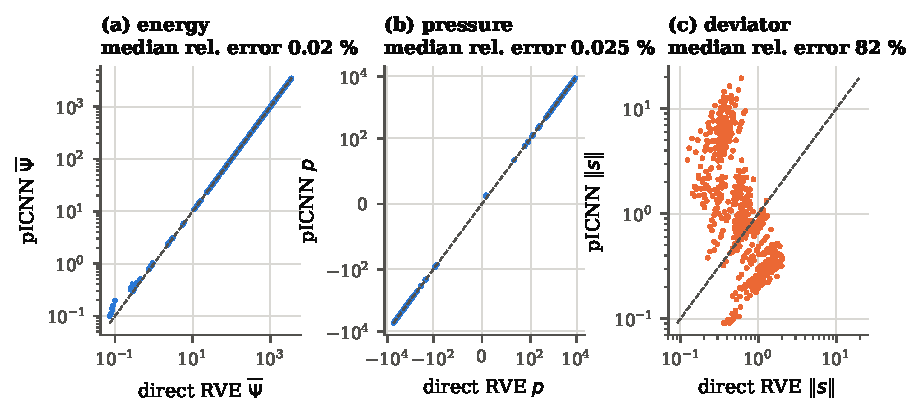
\includegraphics[width=\textwidth]{fig_parity.pdf}
\caption[Parity of the frozen pICNN against direct RVE solutions]{Parity of the frozen pICNN against direct RVE solutions on the Phase~7 test
states: (a) homogenized energy, (b) pressure $p=\tfrac13\operatorname{tr}\bm\sigma$
(symmetric logarithmic axes), (c) norm of the Cauchy stress deviator.}
\label{fig:parity}
\end{figure}

\paragraph{Inference.} Small training and test losses do not certify the model. The loss is dominated by the volumetric
part of the response, which the surrogate reproduces; the deviatoric part is practically not
constrained by it and is the actual weakness. The test losses being of the order of the
training loss shows that the model generalizes over the sampled states, not that it is accurate
in shear.

\section{Surrogate accuracy: two views of the same errors}\label{sec:accuracy}

\paragraph{The conventional view.} Energy and stress errors are commonly reported
as RMSE divided by the training RMS scales $s_\Psi$ and $s_P$. With this metric the
frozen checkpoint shows small errors (\cref{tab:nrmse}).

\begin{table}[htbp]
\centering\small
\caption{Normalized errors of the frozen checkpoint relative to the training scales.}
\label{tab:nrmse}
\begin{tabular}{@{}lrcc@{}}
\toprule
Evaluation set & Records & Energy NRMSE & Stress NRMSE\\
\midrule
Phase 7 independent, test split & 531 & $5.3\times10^{-4}$ & $1.0\times10^{-3}$\\
Fresh holdout, test split & 72 & $3.3\times10^{-4}$ & $8.0\times10^{-4}$\\
Fresh holdout, 30 benchmark cases & 30 & $4.3\times10^{-4}$ & $8.8\times10^{-4}$\\
\bottomrule
\end{tabular}
\end{table}

\paragraph{The physically separated view.} The Cauchy stress
$\bm\sigma=J^{-1}\Pstress\F^{\mathsf T}$ is split into the pressure
$p=\tfrac13\operatorname{tr}\bm\sigma$ and the deviator $\bm s=\bm\sigma-p\Iten$,
and the relative error of each part is evaluated record by record
(\code{figure\_sources\slash{}}, script \code{split\_metrics.py}). The picture changes
completely (\cref{tab:split}, \cref{fig:split}). Pressure is reproduced to a median
of $0.01$--$0.06\,\%$; only in the near-isochoric regime, where $p$ itself is small, does the median rise to $0.9\,\%$. The deviatoric stress, which governs shape
change and therefore everything the matrix does at nearly constant volume, has a
median error of $76$--$83\,\%$ (frozen) and $59$--$84\,\%$ (shear-adapted) outside
the expansion regime. In expansion states, where the deviator is small, the error
exceeds $1000\,\%$.

\begin{table}[htbp]
\centering\small
\caption[Median relative errors of pressure and deviatoric stress, Phase 7 test split]{Median relative errors of pressure and deviatoric stress, Phase~7 independent test split (531 records). RMS $\|\bm s\|$: size of the reference deviator.}
\label{tab:split}
\begin{tabular}{@{}lrcccc@{}}
\toprule
Regime & $n$ & RMS $p_\mathrm{ref}$ & RMS $\|\bm s_\mathrm{ref}\|$ & pressure & deviator\\
& & & & frozen & frozen / shear-adapted\\
\midrule
compression $J<0.7$ & 150 & 4559 & 1.19 & $0.014\,\%$ & $76\,\%$ / $79\,\%$\\
intermediate & 201 & 1927 & 0.67 & $0.055\,\%$ & $80\,\%$ / $62\,\%$\\
near-isochoric $|J-1|<0.02$ & 27 & 88 & 0.57 & $0.91\,\%$ & $80\,\%$ / $59\,\%$\\
expansion $J>1.4$ & 153 & 6774 & 0.36 & $0.029\,\%$ & $1557\,\%$ / $1422\,\%$\\
\midrule
all & 531 & 4528 & 0.79 & $0.025\,\%$ & $83\,\%$ / $84\,\%$\\
\bottomrule
\end{tabular}
\end{table}

\begin{figure}[htbp]
\centering
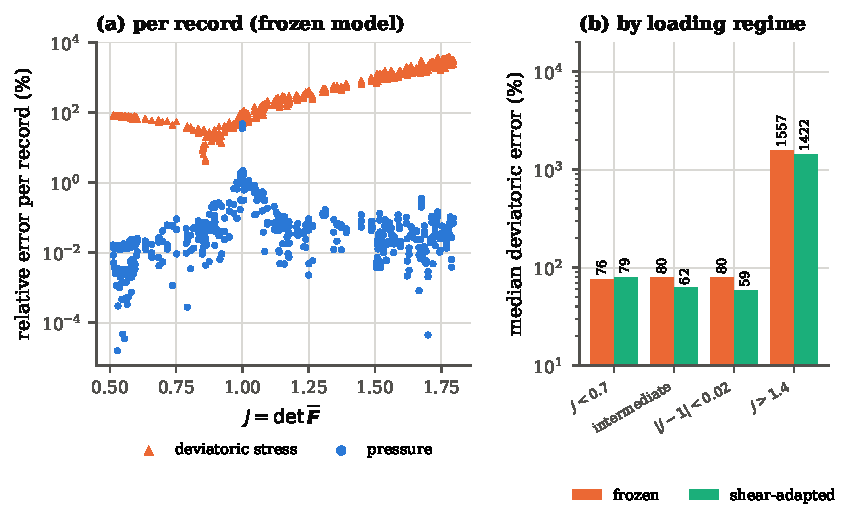
\includegraphics[width=\textwidth]{fig_split_errors.pdf}
\caption[Per-record relative errors of pressure and deviatoric stress against $J$]{(a) Per-record relative errors of pressure and deviatoric stress
against $J$ (frozen checkpoint). The two are separated by four orders of
magnitude. (b) Median deviatoric error by loading regime for both checkpoints.}
\label{fig:split}
\end{figure}

\paragraph{Inference.} The aggregate metric hides the problem: the same checkpoint has errors of order $10^{-4}$ in
pressure and of order $10^{-1}$--$10^{1}$ in the deviator. Acceptance of a surrogate for this
material must therefore be based on separate pressure and deviatoric errors. The fine-tune
does not remove the deviatoric error on the general test states (the difference between the two
checkpoints is within the scatter of the regimes), so it cannot be regarded as a general fix.

\section{Response along five loading paths}\label{sec:paths}

The test-set statistics of \cref{sec:accuracy} mix all loading modes. To see how
the error depends on the mode, the frozen surrogate was evaluated along the five
proportional loading paths of \cref{tab:paths}, from $0$ to $10\,\%$ amplitude and
for the three volume fractions, and compared with direct RVE solutions.

\begin{table}[htbp]
\centering\small
\caption[Proportional loading paths]{Proportional loading paths, amplitude $a\in[0,0.1]$. Direct RVE points:
solves of the earlier validation studies, i.e.\ volume-fraction map and shear-path check (E), and additional solves made for this comparison (N), both with
$h=0.22$ and integration order~10. At $a=0.10$ there is no direct point for uniaxial tension and compression at
$\vfrac=0.05$, and for simple shear only $\vfrac=0.05$ has one.}
\label{tab:paths}
\begin{tabular}{@{}llll@{}}
\toprule
Path & $\Fbar(a)$ & $\overline J$ at $a=0.1$ & Direct RVE points\\
\midrule
uniaxial tension & $\mathrm{diag}(1+a,1,1)$ & 1.100 & $a=0.05$ (E), $0.10$ (N)\\
uniaxial compression & $\mathrm{diag}(1-a,1,1)$ & 0.900 & $a=0.05$ (E), $0.10$ (N)\\
simple shear & $\Iten+a\,\bm e_1\otimes\bm e_2$ & 1.000 & $a=0.025,0.05,0.075$ (E), $0.10$ (N)\\
equibiaxial tension & $\mathrm{diag}(1+a,1+a,1)$ & 1.210 & $a=0.05,0.10$ (N)\\
volumetric expansion & $(1+a)^{1/3}\,\Iten$ & 1.100 & $a=0.05,0.10$ (N)\\
\bottomrule
\end{tabular}
\end{table}

\paragraph{Microscale fields.} \Cref{fig:rvefields} shows what the RVE computes for
two of these paths at $\vfrac=0.10$. Under uniaxial tension the response is
dominated by the volumetric part: the mean pressure is $549$, and the particle
perturbs it by only $-0.13$ to $+0.19$. The fluctuation $\bm w$ concentrates at the poles
of the particle along the loading axis, and the isochoric strain is amplified next
to the particle by a factor of about $2.6$ relative to the median value in the cell. Under simple
shear the pressure perturbation has the antisymmetric four-lobe pattern of a rigid
inclusion in shear, and the fluctuation is a factor of two smaller. The rigid
particle and its periodic images stiffen the matrix only through these local
deviatoric concentrations, which is why the effective shear modulus depends on
$\vfrac$ much more strongly than the bulk modulus.

\begin{figure}[htbp]
\centering
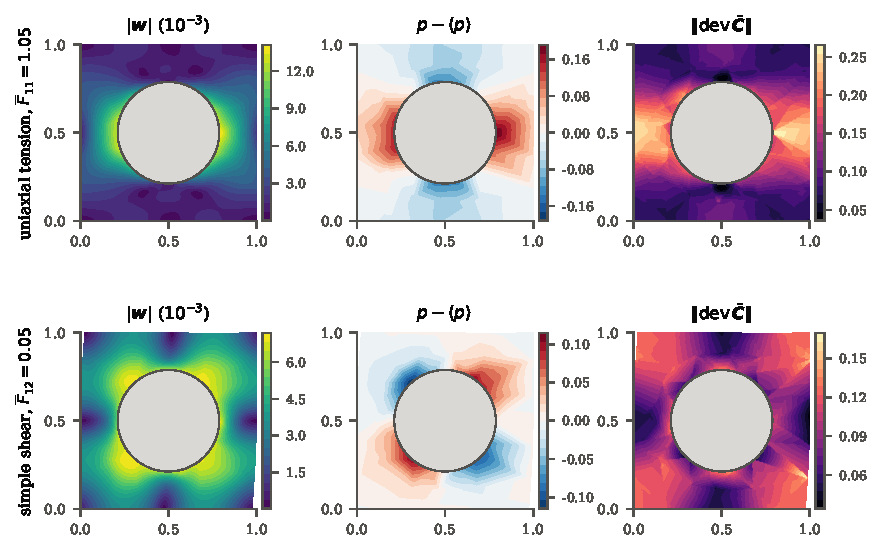
\includegraphics[width=\textwidth]{fig_rve_fields.pdf}
\caption[Direct RVE field solutions for $\vfrac=0.10$]{Direct RVE solutions for $\vfrac=0.10$ ($h=0.22$, order~10), section
$z=0.5$ through the particle centre, deformed configuration. Left: periodic
fluctuation $|\bm w|$. Centre: deviation of the pressure from its mean. Right:
isochoric strain measure $\|\mathrm{dev}\,\bar{\bm C}\|$. Grey: rigid particle.
Top: uniaxial tension $\overline F_{11}=1.05$. Bottom: simple shear $\overline F_{12}=0.05$.}
\label{fig:rvefields}
\end{figure}

\paragraph{Surrogate versus direct RVE.} \Cref{fig:loadpaths} shows the results.
For the four paths with a volume change, the surrogate follows the direct RVE
over the whole range: the relative stress error is between $10^{-4}$ and
$7.8\times10^{-3}$, and the largest energy error is $1.3\,\%$ ($\vfrac=0.10$,
$a=0.05$). Simple shear behaves differently. The surrogate is too stiff by $46\,\%$,
$55\,\%$ and $75\,\%$ for $\vfrac=0.02$, $0.05$ and $0.10$, and these errors are
the same at every amplitude from $2.5$ to $10\,\%$. The shear error is therefore a
wrong effective shear modulus, not a missing nonlinearity, in agreement with the
small-strain moduli of \cref{tab:moduli}. It grows with $\vfrac$ because the
surrogate also overestimates how strongly the shear stiffness depends on the volume
fraction (\cref{fig:vfdep}). From $\vfrac=0.02$ to $0.10$, the direct RVE stiffens by
$7.9\,\%$ in uniaxial tension and by $17\,\%$ in shear. Both values are close to
the Mori--Tanaka estimates of $8.9\,\%$ for $K$ and $22\,\%$ for $\mu$. The surrogate
reproduces the volumetric increase ($7.3\,\%$) but predicts $41\,\%$ in shear, a
factor of 2.4 too much.

\begin{figure}[htbp]
\centering
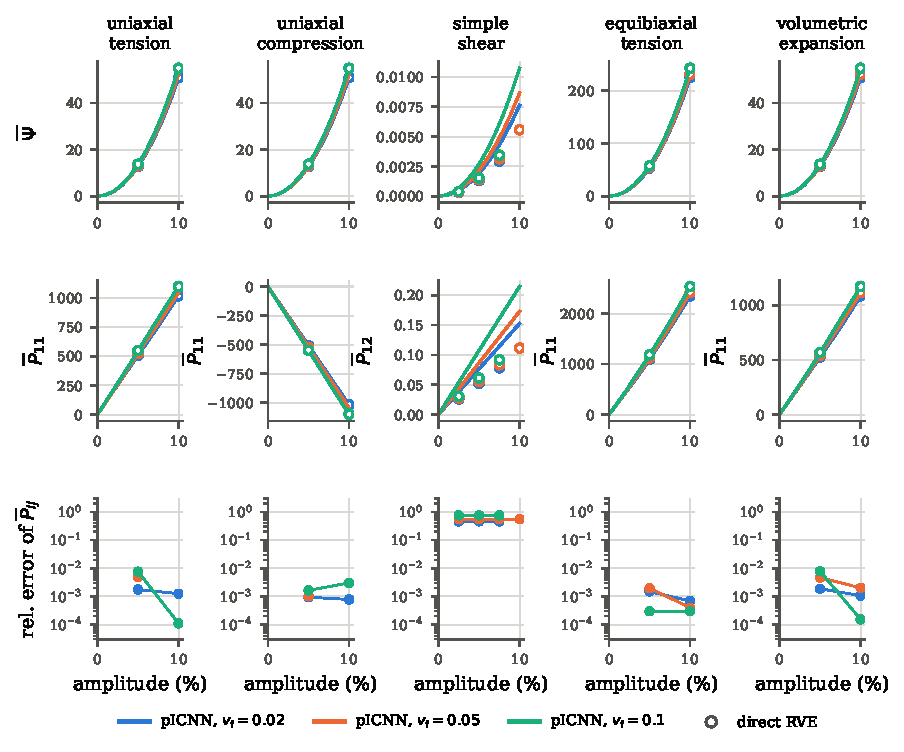
\includegraphics[width=\textwidth]{fig_load_paths.pdf}
\caption[Frozen pICNN and direct RVE along the five loading paths]{Frozen pICNN (lines) and direct RVE (circles) along the five loading paths of
\cref{tab:paths}. Rows: homogenized energy, active stress component, relative error
of that component. Simple shear is the only path without a volume change, and the
only one with a large error.}
\label{fig:loadpaths}
\end{figure}

\begin{figure}[htbp]
\centering
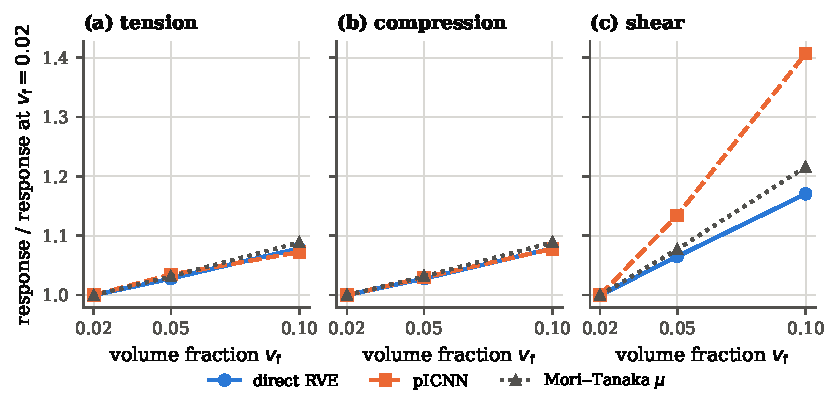
\includegraphics[width=\textwidth]{fig_vf_dependence.pdf}
\caption[Volume-fraction dependence at $5\,\%$ amplitude]{Volume-fraction dependence at $5\,\%$ amplitude, normalized by the value at
$\vfrac=0.02$: direct RVE, pICNN and the Mori--Tanaka ratio of the relevant modulus
(\cref{eq:mt}). (a) $\overline P_{11}$ in uniaxial tension, (b) $|\overline P_{11}|$ in uniaxial
compression, (c) $\overline P_{12}$ in simple shear.}
\label{fig:vfdep}
\end{figure}

\paragraph{Inference.} For loadings with a volume change the surrogate is accurate to within $0.8\,\%$ in stress and $1.3\,\%$ in energy
over the whole amplitude range and all volume fractions, and it follows the dependence on
$\vfrac$. In simple shear, the error is a constant factor at every amplitude, so it is an error of
the effective shear modulus, not of the nonlinearity. This directly motivates the separate
volumetric and isochoric energies of \cref{sec:proposed}.

\section{Diagnosis of the deviatoric error}\label{sec:diagnosis}

The evidence identifies one dominant cause and excludes several others.

\paragraph{Cause: the loss cannot see shear.} By \cref{eq:split}, volumetric and
deviatoric energies differ by the factor $K/\mu\approx10^4$ at comparable strains.
The combined Phase~6/7 dataset contains targeted states down to $J=0.51$ and up to $J=1.80$
(\cref{fig:coverage}). Of its 1671 records, only 90 ($5.4\,\%$) are near-isochoric ($|J-1|<0.02$), and only 111 ($6.6\,\%$) lie in the range $J\in[0.969,1.034]$ of the final $P_1$ states at $5\,\%$ stretch. (For the training split alone, 909 records, the counts are 54 and 63.) The
energy RMS of the combined dataset is $1127$ ($991$ for the training split), of which the isochoric part
$\approx\tfrac{\mu}{2}(\bar I_1-3)$ contributes an RMS of only $0.09$, about
$10^{-4}$. The loss \cref{eq:loss} normalizes by $s_\Psi=979$ and $s_P=2440$. The
decisive number follows directly: on the validation split, replacing the reference
stress by its volumetric part alone, that is \emph{deleting the entire deviatoric
response}, raises the stress loss by $8.1\times10^{-9}$. That is $1.5\,\%$ of the
validation stress loss actually reached ($5.3\times10^{-7}$). The $55\,\%$ error of $\overline P_{01}$ at $5\,\%$ simple shear contributes
only $\approx2\times10^{-11}$ to the stress loss of that record. To the optimizer, a model with
correct shear and a model with no shear are practically indistinguishable. The
relative-Frobenius tangent term has the same blindness, because $\|\Abar\|_F$ is
dominated by entries of order $K$. This is why, at $5\,\%$ shear, the full-tangent
error was only $1.0\,\%$ while the active component
$\partial\overline P_{01}/\partial\overline F_{01}$ was wrong by $55\,\%$
($1.731$ vs.\ $1.115$).

\paragraph{Aggravating factor: non-isochoric features.} The features
$I_1=J^{2/3}\bar I_1$ and $I_2=J^{4/3}\bar I_2$ change mostly with $J$ in the
training data. The same non-negative weights that fit the volumetric response
therefore also set the shear stiffness. The network has no separate degree of
freedom with which it could correct $\mu_{\mathrm{eff}}$ without disturbing $K$.

\paragraph{Excluded causes.} The direct-RVE labels are correct (Mori--Tanaka
agreement, P2-V5/V6). Stress and tangent are exact derivatives of the network
energy (S-V1). The reference state is exact (V2). An earlier feature-space
coverage audit placed the shear states in a \emph{dense} region of the
standardized feature space. This is consistent with the diagnosis: the shear
states are well covered in the features, but in a direction the loss ignores.

\begin{figure}[htbp]
\centering
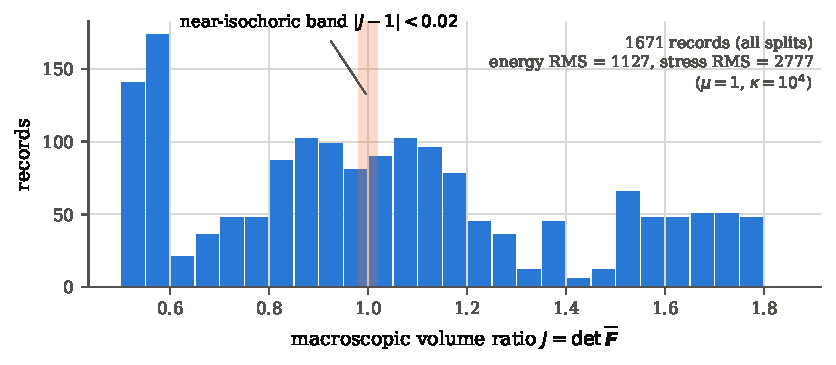
\includegraphics[width=\textwidth]{fig_training_coverage.pdf}
\caption[Determinant distribution of the 1671 records of the combined dataset]{Determinant distribution of the 1671 records of the combined Phase~6/7 dataset (training, validation and test splits). The targeted
compression and expansion tails dominate both the energy and the stress scales;
only $5.4\,\%$ of the records are near-isochoric.}
\label{fig:coverage}
\end{figure}

\section{Proposed surrogate improvements (not implemented)}\label{sec:proposed}

The diagnosis points to three changes. They are specified here for future work;
none of them was implemented or tested in this project.

\paragraph{Volumetric--isochoric energy.} In the present network, $I_1=J^{2/3}\bar I_1$
and $I_2=J^{4/3}\bar I_2$ enter through the same weights as $J$, so a single set of
parameters governs both the bulk and the shear response. An additive split
\begin{equation}
  \widehat\Psi(\F;\vfrac)=\Psi_{\mathrm{iso}}\bigl(\bar I_1,\bar I_2^{3/2};\vfrac\bigr)
  +\Psi_{\mathrm{vol}}(J;\vfrac),\qquad
  \bar I_1=J^{-2/3}I_1,\quad \bar I_2^{3/2}=J^{-2}I_2^{3/2},
  \label{eq:split-proposed}
\end{equation}
with one network per term separates the two. At $\F=\Iten$ the tangent of
\cref{eq:split-proposed} decomposes exactly into a volumetric part governed only by
$\Psi_{\mathrm{vol}}''(1)$ and a deviatoric part governed only by $\Psi_{\mathrm{iso}}$,
so $K_{\mathrm{eff}}$ and $\mu_{\mathrm{eff}}$ become independent quantities. Polyconvexity of
the complete energy follows from four conditions, all of which can be enforced by
construction:
\begin{enumerate}
  \item $\bar I_1$ and $\bar I_2^{3/2}$ are polyconvex functions of
        $\F$~\cite[Lemmas~2.1 and~2.2]{Hartmann2003};
  \item $\Psi_{\mathrm{iso}}$ is convex and non-decreasing in each of its two
        arguments (an ICNN with non-negative weights, as in \cref{sec:architecture}),
        so that the composition is polyconvex;
  \item $\Psi_{\mathrm{vol}}$ is convex in $J=\det\F$, and is therefore polyconvex;
        including $-\ln J$ as a feature with non-negative weight gives
        $\Psi_{\mathrm{vol}}\to\infty$ for $J\to0^{+}$;
  \item a sum of polyconvex functions is polyconvex.
\end{enumerate}
The normalization also separates. Because $\partial\bar I_1/\partial\F$ and
$\partial\bar I_2/\partial\F$ vanish at $\F=\Iten$, the isochoric part is stress-free
in the reference state by construction and needs only an energy offset. The
volumetric part is normalized by
$\Psi_{\mathrm{vol}}(J)-\Psi_{\mathrm{vol}}(1)-\Psi_{\mathrm{vol}}'(1)(J-1)$, which is affine in
$J$ and therefore preserves convexity and objectivity, as in \cref{eq:norm}.

\paragraph{Balanced loss.} The stress term of \cref{eq:loss} would be replaced by
separately normalized pressure and deviatoric terms,
\begin{equation}
  \mathcal L=w_\Psi\mathcal L_\Psi+w_p\,\frac{\langle(\hat p-p)^2\rangle}{s_p^2}
  +w_s\,\frac{\langle\Vert\operatorname{dev}\hat{\bm\sigma}-\operatorname{dev}\bm\sigma\Vert^2\rangle}{s_s^2}
  +w_A\mathcal L_A,
  \label{eq:loss-proposed}
\end{equation}
where $s_p$ and $s_s$ are the RMS values of the pressure and of the deviatoric-stress
norm in the training split. Both stress terms are then $O(1)$, so the deviatoric
response can no longer be neglected at the cost of $1.5\,\%$ of the loss, as found
above. The same scaling would apply to a split tangent term.

\paragraph{Sampling and metrics.} Training states would be sampled in the range of
$J$ consistent with $\kappa/\mu$ (the macroscopic runs stayed within
$J\in[0.969,1.034]$), with dense isochoric coverage instead of the present
$5.4\,\%$. Pressure error, deviatoric error, $K_{\mathrm{eff}}$ and $\mu_{\mathrm{eff}}$
(\cref{tab:split}) would be the primary acceptance measures, with the aggregate
NRMSE reported only alongside them. The split energy would also supply the separate
volumetric term that a mixed macroscopic formulation requires (\cref{sec:macro}).

\section{Shear fine-tuning}

The shear-adapted checkpoint was fitted on 18 of 33 additional simple-shear records
(6 more served for validation and 9 as a development test set), with the original data
replayed; the settings are in \cref{tab:trainconf}. The adaptation variants were compared on the
development set and the context holdout; the selected model was then evaluated, after it
had been frozen, on 12 new simple-shear cases generated afterwards. These cases use amplitudes
$\gamma=0.015$, $0.0325$, $0.0725$ and $0.0975$, all three volume fractions, and a
microstructure seed different from the adaptation data.

\begin{table}[htbp]
\centering\small
\caption{Final shear holdout (12 cases): mean relative errors.}
\label{tab:shear}
\begin{tabular}{@{}lccc@{}}
\toprule
Checkpoint & $\overline P_{01}$ & $\partial\overline P_{01}/\partial\overline F_{01}$ & energy\\
\midrule
frozen & $58.8\,\%$ & $58.7\,\%$ & $58.8\,\%$\\
shear-adapted & $40.1\,\%$ & $40.0\,\%$ & $40.1\,\%$\\
\bottomrule
\end{tabular}
\end{table}

The three errors are almost identical and independent of the amplitude: for the
frozen model, $58.7$--$58.8\,\%$ at every $\gamma$. This is the signature of a wrong
small-strain shear modulus rather than of a nonlinear misfit, in exact agreement
with \cref{tab:moduli}. Fine-tuning lowered $\mu_{\mathrm{eff}}$ by about $12\,\%$
and the error from $59\,\%$ to $40\,\%$ (\cref{fig:shear}). It did not, however,
improve the deviatoric error on the general Phase~7 states (median $83\,\%$ to
$84\,\%$, \cref{tab:split}). As the diagnosis predicts, the fine-tune moves the
shear modulus where shear data are added, but cannot fix a loss that is
insensitive to shear.

\begin{figure}[htbp]
\centering
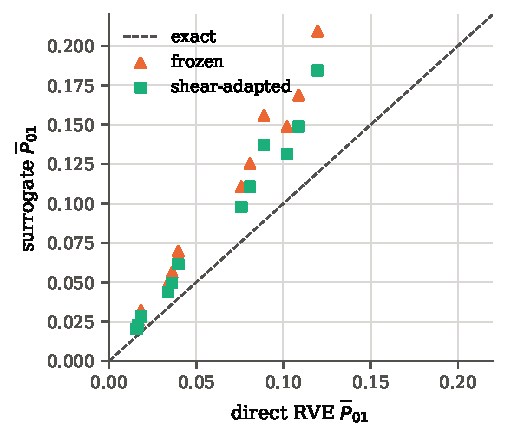
\includegraphics[width=0.48\textwidth]{fig_shear_holdout.pdf}
\caption[Final shear holdout: surrogate versus direct RVE]{Final shear holdout: surrogate versus direct RVE $\overline P_{01}$ for
12 unseen cases. Both checkpoints overestimate the shear stress by a nearly
constant factor.}
\label{fig:shear}
\end{figure}

\paragraph{Other evaluations of the frozen model, reinterpreted.} A loading-path
sweep (five modes, eleven amplitudes, 165 points) confirmed work conjugacy to
$4.6\times10^{-6}$ and tangent symmetry to $1.5\times10^{-15}$. An inverse design
of $\vfrac$ for target responses at $5\,\%$ loading succeeded for uniaxial
stretch (3/3 targets, $\le0.24\,\%$ error) and compression (3/3, $\le2.1\,\%$), but
not for simple shear: all shear targets lay outside the predicted range, and only one of three
reached the tolerance (at the lower bound of $\vfrac$). A sampled
acoustic-tensor screen (655 directions) found positive minima for both the
surrogate and the direct RVE. All these observations are consistent with the
diagnosis. Uniaxial states with $J\neq1$ are pressure-dominated and therefore well
predicted, whereas isochoric shear is not.

\paragraph{Inference.} The study shows that the shear error can be reduced only where shear data are added
($59\,\%\to40\,\%$), and that the remaining error is again a constant factor. This supports the
diagnosis that the loss, not the data volume or the architecture alone, limits the shear
accuracy. The fine-tuned checkpoint is a better shear model, but it is not a validated
substitute for the missing shear sensitivity of the loss.

% ======================================================================
\paragraph{Two other adaptation variants.}\label{sec:shearvariants}
Two further variants were trained from the same frozen checkpoint, with the same shear
data and original-data replay, before the full fine-tune was chosen. In the
\emph{context-only adapter} the invariant backbone is frozen and only the volume-fraction
context sub-network is trained (learning rate $10^{-5}$, seed $20261118$, extra weight $3$
on the low-amplitude shear tangent and on the identity tangent, selection restricted to a
loss of at most $2\,\%$ in original validation). On 12 new shear cases with amplitudes
disjoint from the adaptation data, it lowered the mean $\overline P_{01}$ error from
$58.8\,\%$ to $51.4\,\%$, against $40.1\,\%$ for the full fine-tune on the same cases;
these cases reuse the microstructure seed of the adaptation data. In the
\emph{shear-tangent calibration} (learning rate $2\times10^{-5}$, seed $20261117$) no
epoch improved on the starting model in the selection score, so the best epoch was
epoch~0 and the checkpoint remained identical to the frozen one. Only the full fine-tune, in which every
parameter may change, produced a clear reduction, and it is the variant used in the
following chapters. The reason why the other two failed was not investigated.

\section{Macroscopic application and volumetric locking}\label{sec:macro}

\paragraph{Results.} With the frozen surrogate ($\vfrac=0.05$), the clamped cube
of \cref{sec:macro-method} was solved with linear ($P_1$) and quadratic ($P_2$)
elements on three meshes (\cref{tab:macro}, \cref{fig:macro}). The $P_1$ runs
completed all 100 increments to $5\,\%$ stretch. The $P_2$ runs completed $0.5\,\%$ on
all meshes and $1\,\%$ on two of them; the $1\,\%$ run on the finest mesh stopped at
$0.70\,\%$ after 18 increments. All accepted states are converged to
$\|\bm R_\mathrm{free}\|<10^{-8}$ and orientation-preserving.

\begin{table}[htbp]
\centering\small
\caption[Macroscopic runs: energy, volume ratio and Newton effort]{Macroscopic runs: stored energy at the common stretch $\varepsilon=0.5\,\%$,
volume-ratio range and Newton effort. Free-uniaxial reference
$\tfrac32\mu_{\mathrm{eff}}\varepsilon^2$: $6.5\times10^{-5}$ with the pICNN
$\mu_{\mathrm{eff}}=1.731$.}
\label{tab:macro}
\begin{tabular}{@{}lrrrccr@{}}
\toprule
Order & $h$ & elements & DOFs & $\int\Psi\dd V$ at $0.5\,\%$ & $J_{\min}$ at $0.5\,\%$ & Newton it./step\\
\midrule
$P_1$ & 0.25 & 399 & 405 & $7.57\times10^{-3}$ & 0.99683 & 20.1\\
$P_1$ & 0.20 & 648 & 642 & $3.57\times10^{-3}$ & 0.99675 & 23.2\\
$P_1$ & 0.16 & 1818 & 1356 & $2.06\times10^{-3}$ & 0.99796 & 30.8\\
\midrule
$P_2$ & 0.25 & 399 & 2334 & $8.54\times10^{-5}$ & 0.99994 & 62.0\\
$P_2$ & 0.20 & 648 & 3759 & $8.36\times10^{-5}$ & 0.99994 & 81.4\\
$P_2$ & 0.16 & 1818 & 8928 & $8.29\times10^{-5}$ & 0.99985 & 101.3\\
\bottomrule
\end{tabular}
\end{table}

\begin{figure}[htbp]
\centering
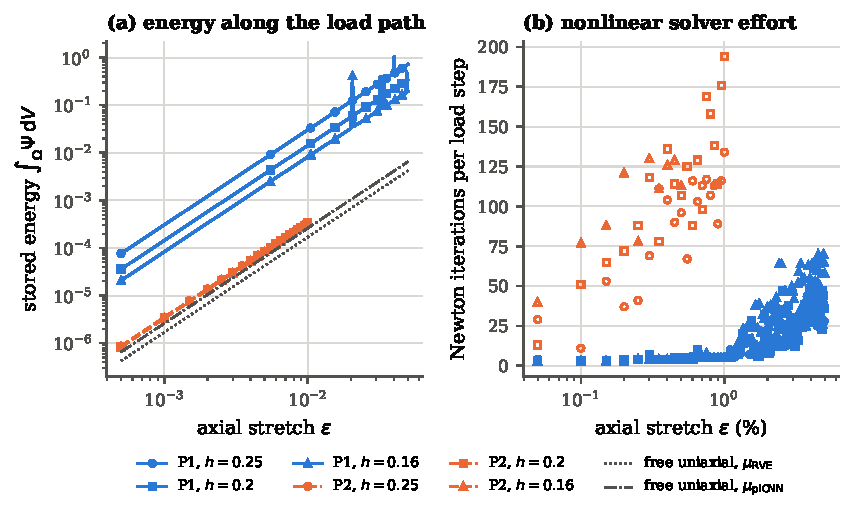
\includegraphics[width=\textwidth]{fig_macro_energy.pdf}
\caption[Macroscopic runs]{Macroscopic runs. (a) Stored energy along the load path. All curves grow
as $\varepsilon^2$, but the $P_1$ energies lie 25--89 times above the $P_2$ energies
and the analytical free-uniaxial estimates, and decrease strongly under
refinement; the $P_2$ energies change by $2.2\,\%$ and $0.8\,\%$. (b) Newton
iterations per load step.}
\label{fig:macro}
\end{figure}

\paragraph{Interpretation: the $P_1$ solution is locked.} Three independent
observations show that the $P_1$ energies are not physical.
\begin{enumerate}
  \item \emph{Magnitude.} At equal stretch, the $P_1$ energy exceeds the $P_2$ energy
        by factors of 89, 43 and 25 on the three meshes. The $P_2$ value is only
        $1.3$ times the analytical free-uniaxial estimate, a plausible stiffening
        for clamped ends.
  \item \emph{Mesh dependence.} The $P_1$ energy roughly halves with each refinement
        and converges very slowly towards the $P_2$ value. The $P_2$ value changes
        by only $2.2\,\%$ and $0.8\,\%$.
  \item \emph{Spurious volume change.} With an effective $K/\mu\approx10^4$, the
        $P_1$ solution still shows $J_{\min}=0.997$ at $0.5\,\%$ stretch, and
        $J\in[0.969,1.034]$ at $5\,\%$ on the coarsest mesh ($[0.969,1.030]$ and $[0.980,1.023]$ at $h=0.20$ and $0.16$). At $0.5\,\%$ the local volume changes are
        14--51 times larger than with $P_2$ (ratio of $1-J_{\min}$ on the three meshes).
\end{enumerate}
This is classical volumetric locking. Linear tetrahedra cannot represent
near-isochoric deformation fields~\cite{Simo1985,Zienkiewicz2013}. The RVE avoids
locking through its mixed $P_2/P_1$ formulation, but the macroscopic solver is
displacement-only. The $P_1$ result therefore demonstrates robust \emph{solver
integration} of the surrogate up to $5\,\%$, not a converged component response.

\paragraph{Interpretation: why $P_2$ is hard to drive.} The $P_2$ discretization is
far less locked, but its stiffness matrix inherits a condition number of
$3.3\times10^4$ (M-V0), of the order of the bulk-to-shear ratio $\kappa/\mu=10^4$. Starting from the affine predictor, the full
Newton step overshoots into inadmissible states ($J<0$ at some quadrature points).
The energy line search and the spectral shift then take many damped steps before
the final, quadratically convergent iterations; for example, the residuals
$9.1\times10^{-4}\to5.4\times10^{-5}\to2.5\times10^{-8}\to2.4\times10^{-13}$ close the
first increment at $h=0.25$. This explains the 62--137 iterations per increment. It
is a property of a displacement-only formulation of a nearly incompressible law,
not a defect of the surrogate.

\paragraph{Three distinct difficulties.} The macroscopic results combine three
effects with different causes and remedies.
\begin{enumerate}
  \item \emph{Volumetric locking} is a discretization error of the $P_1$
        interpolation: the displacement space cannot represent nearly
        volume-preserving, non-uniform fields. A uniform deformation is represented
        exactly (patch test V5), so the locking arises from the non-uniform field
        induced by the clamped faces. Evidence: the energy ratio, the mesh dependence
        and the spurious volume change listed above. Remedy: a mixed $u$--$p$ or
        $\bar{\bm F}$ formulation, or higher-order elements.
  \item \emph{Ill-conditioning} is an algebraic property: the stiffness matrix of a
        nearly incompressible material has eigenvalues spread by about $K/\mu$ (condition
        estimate $3.3\times10^4$, M-V0). It affects $P_1$ and $P_2$ alike and does not
        by itself make a solution inaccurate; with the sparse direct solver used here
        the residuals still reach $10^{-13}$. It would limit iterative linear solvers.
        Remedy: direct factorization or a block preconditioner.
  \item \emph{Inadmissible Newton states} are a nonlinear-solver issue: full steps from
        the affine predictor reach $J\le0$ at some quadrature points. The line search
        and spectral shift recover convergence at the cost of many iterations, and the
        finest $P_2$ run stopped at $0.70\,\%$. Remedy: better predictors, smaller
        increments or $J$-safeguarded updates.
\end{enumerate}
A mixed formulation addresses the first difficulty. It does not remove the other two
automatically: it leads to a saddle-point system, which requires an inf--sup stable
pair of spaces~\cite{Boffi2013} and a suitable linear solver, and its Newton iterations
still need globalization.

\paragraph{Consequences.} (i) A mixed $u$--$p$~\cite{Simo1985} or $\bar{\bm F}$~\cite{deSouzaNeto1996} macroscopic
formulation, which the project already implements at the RVE
level, is required for meaningful component responses. A mixed form of the type
\cref{eq:mixed} needs the volumetric part of the energy as a separate term; the
present single-network energy does not provide it, whereas the split energy
\cref{eq:split-proposed} does. The proposed surrogate change is therefore a
prerequisite for the proposed macroscopic formulation. (ii) The deviatoric bias of
\cref{sec:diagnosis} carries over to the macro scale: with the direct-RVE shear
modulus, the energy would be about $35\,\%$ lower ($1.124$ vs.\ $1.731$). (iii) The
shear-adapted checkpoint ran through the identical $P_1$ path. Its final energy
differs by only $0.65\,\%$, as expected for a locked, volumetrically dominated
solution.

\paragraph{Inference.} The surrogate can be integrated robustly into a finite-element solver (all $P_1$ runs reach $5\,\%$
stretch, all accepted states are converged and orientation-preserving), but the displacement-only
macroscopic model cannot give a converged component response for a nearly incompressible
material: the $P_1$ energies are locked, and the $P_2$ runs are limited by the nonlinear solver.
No statement about component-level accuracy of the surrogate is therefore possible from these
runs. They demonstrate integration and the required next step, a mixed formulation, but not
macroscopic accuracy.

\chapter{Computation Time Study and Bottlenecks}\label{ch:performance}

The approach moves the cost of the microscale from the macroscopic solve into an
offline phase. Its efficiency is therefore decided by a chain of four costs:
(i)~the direct RVE solves that generate the training data, (ii)~the constitutive
evaluation per macroscopic Newton iteration, (iii)~the number of Newton iterations
the macroscopic problem needs, and (iv)~the resulting overall budget compared with
a concurrent FE$^2$ computation. This chapter quantifies each link and identifies
the bottleneck at each stage (\cref{fig:bottlenecks}). Memory is not a limiting
factor at the problem sizes considered: the largest macroscopic model has
83\,628 quadrature points and the RVE systems have at most 7518 unknowns.

All timings are measured by the program itself: by stage
timers built into the bridge (\code{TIMINGS} in \code{src\slash{}ngsolve\_umat.py}),
by the timing benchmark \code{benchmarks\slash{}rve\_surrogate\_rve\_benchmark.py}, and by
the dataset generator. Newton iteration counts are taken from the stored run
reports. No timing was taken by hand.

\begin{figure}[htbp]
\centering
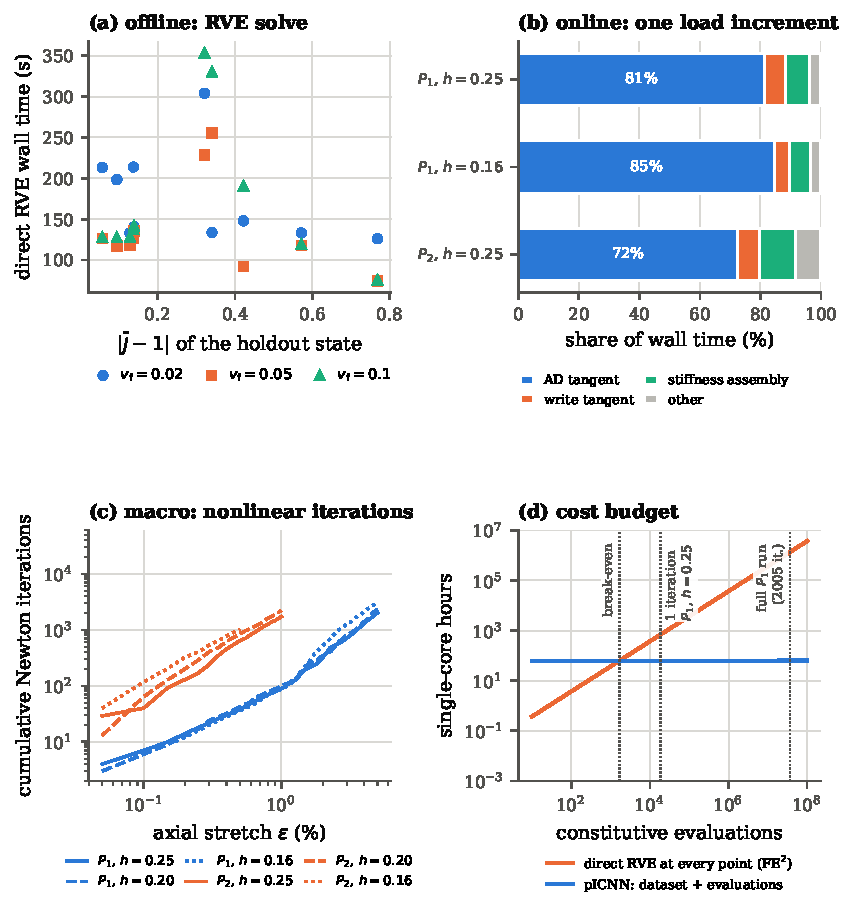
\includegraphics[width=\textwidth]{fig_bottlenecks.pdf}
\caption[Bottlenecks of the approach]{Bottlenecks of the approach. (a) Offline: wall time of one direct RVE
evaluation for the 30 benchmark cases versus the distance $|\overline J-1|$ of the state from
the reference configuration; the spread is not explained by $|\overline J-1|$ (Spearman
$\rho=-0.15$). (b) Online: stage shares of the bridge for the first load increment
(\cref{tab:profile}). (c) Macroscopic solve: cumulative Newton iterations along the
load path of the stored runs ($P_2$, $h=0.16$: run to $0.5\,\%$). (d) Overall budget:
single-core hours for $N$ constitutive evaluations, direct RVE at every evaluation
($134\,$s each, without tangent) versus the surrogate (1671 dataset solves plus
$36\,\mu$s per evaluation including the tangent).}
\label{fig:bottlenecks}
\end{figure}

\section{Offline cost: direct RVE versus surrogate}

The paired benchmark on 30 fresh-holdout cases (one thread, cluster node, two
repeats per direct RVE, fifteen per surrogate) gives the timings in
\cref{tab:timing} and \cref{fig:timing}. One direct RVE evaluation requires the
free-rotation equilibrium plus energy and stress recovery. It takes a median of
$134\,$s, ranging from $75\,$s to $353\,$s depending on the load path and the
continuation steps needed. Mesh generation is negligible ($0.08$--$0.10\,$s per
volume fraction). The surrogate evaluates energy and stress in $2.3\,$ms. The
median paired speed-up is $5.78\times10^4$ (10th--90th percentile
$5.0\times10^4$--$1.1\times10^5$). If the one-off reference-state evaluation of the
network is amortized over the 30 cases, it is $2.7\times10^3$. Generating the
1671-record dataset therefore costs of the order of $1671\times134\,\mathrm{s}\approx62$
single-core hours, before tangents.

\begin{table}[htbp]
\centering\small
\caption{Measured cost of one constitutive evaluation (energy + first Piola stress).}
\label{tab:timing}
\begin{tabular}{@{}lrr@{}}
\toprule
Quantity & Median & Range / note\\
\midrule
direct RVE, $\vfrac=0.02$ & $144\,$s & $126$--$304\,$s\\
direct RVE, $\vfrac=0.05$ & $122\,$s & $75$--$255\,$s\\
direct RVE, $\vfrac=0.10$ & $133\,$s & $76$--$353\,$s\\
pICNN, energy + stress & $2.3\,$ms & per case, 1 thread\\
paired speed-up (solver work) & $5.78\times10^4$ & P10--P90: $5.0\times10^4$--$1.1\times10^5$\\
paired speed-up (incl.\ reference setup) & $2.73\times10^3$ & conservative\\
12-state generation benchmark, 1 vs.\ 12 workers & $1710\,$s / $513\,$s & speed-up $3.3$, efficiency $28\,\%$\\
\bottomrule
\end{tabular}
\end{table}

\begin{figure}[htbp]
\centering
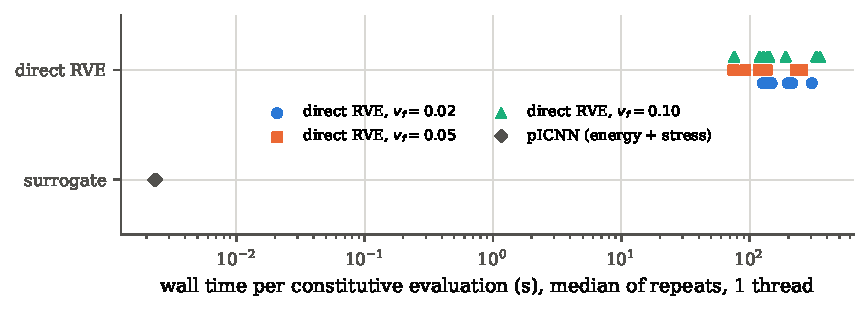
\includegraphics[width=\textwidth]{fig_timing.pdf}
\caption[Wall time per constitutive evaluation, 30 benchmark cases]{Wall time per constitutive evaluation for the 30 benchmark cases: direct
RVE (by volume fraction) versus pICNN. Note the logarithmic axis: the two groups
are separated by almost five decades.}
\label{fig:timing}
\end{figure}

\paragraph{Offline bottleneck.} Dataset generation is the dominant cost of the
whole approach, and its parallel efficiency is low (28\,\% on 12 workers). The
solve times spread by a factor of 4.7 (75--353\,s), and the slowest case takes
2.6 times the median. A few continuation-heavy states therefore dominate the
makespan of a statically partitioned job. \Cref{fig:bottlenecks}(a) shows that
this difficulty cannot be predicted from the size of the deformation: the solve
time is uncorrelated with $|\overline J-1|$. The cost is set instead by the number of
load-continuation steps and rotation updates a state needs, which is known only
after the solve. Sorting the states before distribution would therefore not help.
Dynamic scheduling (a shared work queue with one state per task) is the effective
remedy. The recorded run metadata do not allow start-up and file-system
contributions to be separated from this effect.

\paragraph{Inference.} The surrogate is faster than the direct RVE by a factor of about $2.7\times10^3$ (conservative,
including reference setup) to $5.8\times10^4$ for the constitutive evaluation. This holds for the
tested cases and computing setup only; the saving is real only if many evaluations are needed, because
the data generation is paid once and dominates the total cost.

\section{Online cost: profile of the macroscopic bridge}

\Cref{tab:profile} lists the stage timings for the first load increment of the
macroscopic problem, run with one thread in the local environment
(\code{python -m benchmarks.profile\_bridge}).
This is a separate profiling run; its Newton-iteration counts are those of that run and are not the cluster-run iteration counts of \cref{sec:macro}.

\begin{table}[htbp]
\centering\small
\caption[Built-in stage timings of the bridge, first load increment]{Built-in stage timings of the bridge, first load increment, frozen pICNN, one thread. Shares refer to the total wall time.}
\label{tab:profile}
\begin{tabular}{@{}lrrr@{}}
\toprule
& $P_1$, $h=0.25$ & $P_1$, $h=0.16$ & $P_2$, $h=0.25$\\
\midrule
quadrature points / Newton iterations & 18\,354 / 3 & 83\,628 / 3 & 18\,354 / 25\\
\midrule
1 interpolate and gather $\F$ & $0.6\,\%$ & $0.6\,\%$ & $1.1\,\%$\\
2 pICNN energy, stress, tangent (AD) & $\mathbf{81.4\,\%}$ & $\mathbf{84.7\,\%}$ & $\mathbf{72.4\,\%}$\\
3 write tangent to quadrature points & $6.9\,\%$ & $5.1\,\%$ & $7.3\,\%$\\
4 residual assembly & $0.2\,\%$ & $0.2\,\%$ & $0.3\,\%$\\
5 stiffness assembly & $8.0\,\%$ & $6.8\,\%$ & $11.9\,\%$\\
6 sparse direct solve (UMFPACK) & $0.1\,\%$ & $0.1\,\%$ & $0.8\,\%$\\
other (Python control, line search) & $2.8\,\%$ & $2.6\,\%$ & $6.2\,\%$\\
\midrule
total wall time & $5.7\,$s & $29.7\,$s & $70.4\,$s\\
AD cost per quadrature point & $36\,\mu$s & $43\,\mu$s & $28\,\mu$s\\
\bottomrule
\end{tabular}
\end{table}

\paragraph{Bottleneck.} Between 72 and 85\,\% of the time is spent in the
constitutive evaluation, and almost all of that in the tangent. The nine
reverse-mode passes through a graph with \code{create\_graph=True} cost about
$30$--$40\,\mu$s per quadrature point. Data transfer and assembly together take
about 15\,\%. The sparse solve is negligible at these problem sizes. The cost
scales linearly with the number of quadrature points: $4.6\times$ the points give
$5.5\times$ the AD time. The $P_2$ increment is expensive only because of its 25
Newton iterations (\cref{sec:macro}); per assembly it is as cheap as $P_1$.

\section{Macroscopic solve: number of Newton iterations}

Per iteration, the online cost is small. The total online cost, however, is the
product of this cost and the number of Newton iterations, and the latter is the
bottleneck of the macroscopic stage (\cref{fig:bottlenecks}(c)). The first
increment of the $P_1$ model converges in three iterations, but the iteration count
per step grows along the load path: reaching $5\,\%$ stretch in 100 increments
took 2005, 2318 and 3084 iterations for $h=0.25$, $0.20$ and $0.16$, with up to
47--70 iterations in a single increment. The $P_2$ models need 620--1013
iterations for the first $0.5\,\%$ and 1716--2472 iterations to reach about
$1\,\%$, with up to 194 iterations per increment. The $P_2$ run on the finest mesh
stopped at $0.70\,\%$ when it reached its 24-hour wall-time limit. With the measured
cost of about $1.9\,$s per Newton iteration (seven residual-and-tangent evaluations
in three iterations, \cref{tab:profile}), the $P_1$, $h=0.25$ run corresponds to
roughly one hour of single-core time. The iteration count is driven by
the stiffness ratio $\kappa/\mu\approx10^4$ of the surrogate and by the
conditioning it causes (\cref{sec:macro}), not by the cost of the network. A
faster tangent alone therefore cannot make the $P_2$ runs feasible. The mixed
macroscopic formulation of \cref{sec:proposed} addresses the iteration count
directly.

\paragraph{Inference.} The constitutive evaluation is not the limiting cost of a macroscopic run; the number
of Newton iterations is. An even faster network would therefore change the total cost little, while a
better-conditioned macroscopic formulation would.

\section{Overall cost budget}

\Cref{fig:bottlenecks}(d) combines the offline and online costs. The 1671 dataset
solves cost the same as 1671 direct evaluations, so the surrogate breaks even
after 1671 constitutive evaluations. This is less than one tenth of a single
Newton iteration of the coarsest macroscopic model (18\,354 quadrature points).
The complete $P_1$, $h=0.25$ run evaluated the material law about
$3.7\times10^7$ times. Concurrent FE$^2$ would have needed about $1.4\times10^6$
single-core hours for these evaluations, without the RVE tangents. The surrogate
needed about 63 single-core hours: 62 for generating the data and about one for
the macroscopic run itself.
The training time is not included because it was not recorded consistently;
it does not change the order of magnitude.

\paragraph{Perspective.} One residual-and-tangent evaluation of the $P_1$, $h=0.25$
model costs $\approx0.8\,$s. The corresponding concurrent FE$^2$ iteration on the same mesh would require
18\,354 RVE solves of $\approx134\,$s each, roughly $2.5\times10^6\,$s or about
28~days on one core, still without the RVE tangents. Even with perfect
parallelization on 1000 cores, this would be about 40~minutes per evaluation. The
offline surrogate turns an intractable computation into a seconds-long one. This
is the central benefit of the approach, independent of the accuracy issue of
\cref{sec:diagnosis}.

\paragraph{Summary of the bottlenecks.} Offline, the cost is set by the number
and difficulty of the direct RVE solves, and its parallel execution by load
imbalance. Online, the cost per iteration is set by the AD tangent, and the total
cost by the Newton iteration count of the stiff macroscopic problem. Optimizing
the tangent shortens each iteration by at most a factor of four to seven (the
reciprocal of the non-AD share in \cref{tab:profile}); reducing the
iteration count with a mixed formulation, and the data cost with dynamic
scheduling and active sampling, have the larger potential.

\paragraph{Possible optimizations.} (i) Compute the tangent with a vectorized
Hessian (\code{vmap} over \code{hessian} from \code{torch.func}), or analytically through the
invariants,
\[\Aten=\sum_{a,b}\Psi_{,ab}\,\partial_{\F}y_a\otimes\partial_{\F}y_b
+\sum_a\Psi_{,a}\,\partial^2_{\F}y_a .\]
Only the $4\times4$ Hessian in feature space
then has to come from AD, which should remove most of stage~2. (ii) Write $\Aten$
with a single bulk copy instead of 81 component loops (stage~3). (iii) Reuse the
symbolic structure of the bilinear form across iterations (stage~5).

\chapter{Conclusion}\label{ch:conclusion}

\paragraph{Summary.} The project implemented a complete offline multiscale
pipeline for rigid-particle-reinforced PDMS in Python. \Cref{tab:status} separates
what was achieved, what was implemented without fully meeting its objective, and
what is proposed but not implemented.

{\small
\begin{xltabular}{\textwidth}{@{}p{2.6cm}X@{}}
\caption{Status of the project components.}\label{tab:status}\\
\toprule
Status & Components\\
\midrule
\endfirsthead
\caption[]{\emph{(continued)}}\\
\toprule
Status & Components\\
\midrule
\endhead
\bottomrule
\endfoot
Achieved (implemented and verified) &
  Periodic finite-strain RVE with mixed near-incompressible matrix and exactly
  rigid, freely rotating particle; reaction-based Hill--Mandel homogenization;
  exact Schur-condensed homogenized tangent; reproducible, leak-free dataset
  generation; polyconvex, volume-fraction-conditioned neural energy with objective
  normalization; PyTorch--NGSolve bridge with energy, stress and full $9\times9$
  tangent; 26 passing verification tests (\cref{tab:vmatrix}); RVE moduli within
  $1.1\,\%$ of Mori--Tanaka; median speedup of $5.8\times10^4$ for repeated RVE
  evaluations in the tested setting (\cref{ch:performance}).\\
Partially achieved &
  Surrogate accuracy: accurate in energy and pressure, but not in deviatoric stress
  (\cref{sec:accuracy}); shear fine-tuning reduced but did not remove the error.
  Macroscopic application: $P_1$ reaches $5\,\%$ stretch but is locked, $P_2$ reaches
  $1\,\%$ on two of three meshes (\cref{sec:macro}). No experimental validation.\\
Proposed (not implemented) &
  Volumetric--isochoric surrogate with balanced loss and targeted sampling
  (\cref{sec:proposed}); mixed $u$--$p$ macroscopic formulation (\cref{sec:macro}).\\
\end{xltabular}
}

The speedup and the accuracy are separate results: the speedup shows that the
surrogate is cheap to evaluate, not that its constitutive response is correct.

\paragraph{Main findings.}
\begin{enumerate}
  \item The surrogate is accurate in pressure (median error $0.03\,\%$) but not in
        deviatoric stress (median $76$--$83\,\%$ outside expansion states). Its small-strain shear modulus is
        $46$--$70\,\%$ too high. The cause is quantified: with $\kappa/\mu=10^4$,
        volumetric terms dominate the training loss, and deleting the whole
        deviatoric response changes the stress loss by only $1.5\,\%$. The headline
        training-scale NRMSE of $\sim10^{-3}$ is correct but blind to this error.
        Along five loading paths the four paths with a volume change agree with the
        direct RVE to better than $1\,\%$ in stress, while the simple-shear error is
        constant from $2.5$ to $10\,\%$ amplitude: a wrong modulus, not a missing
        nonlinearity (\cref{sec:paths}).
  \item Shear fine-tuning reduced the shear-holdout error from $59\,\%$ to $40\,\%$ by
        lowering $\mu_{\mathrm{eff}}$. It did not change the general deviatoric
        error, consistent with the diagnosis.
  \item The $P_1$ macroscopic solution to $5\,\%$ stretch is volumetrically locked
        (energy 25--89 times the $P_2$ value). The $P_2$ solution is plausible but
        hard to drive beyond $1\,\%$ because of the $\kappa/\mu$ conditioning of a
        displacement-only formulation.
  \item The computational bottlenecks are the offline RVE solves (62 single-core
        hours, poorly balanced across workers) and, online, the Newton iteration
        count of the stiff macroscopic problem (2005--3084 iterations for $P_1$); the
        AD tangent dominates only the cost of each iteration (\cref{ch:performance}).
  \item Testing caught genuine defects that accuracy metrics could not reveal. The
        Phase~1 network is not frame-indifferent (three negative stiffness
        eigenvalues, V0d) and its shear modulus is $12\,\%$ too low (V8), hidden behind a
        $3\,\%$ stress error. The Phase~5 surrogate failed objectivity (S-V1).
\end{enumerate}

\paragraph{Outlook.} The next steps follow directly from these findings:
(i) the volumetric--isochoric energy \cref{eq:split-proposed} with the balanced
loss \cref{eq:loss-proposed}; (ii) sampling restricted to
physically relevant $J$ with dense isochoric coverage; (iii) a mixed $u$--$p$ or
$\bar{\bm F}$ macroscopic formulation, re-using the RVE's Taylor--Hood
implementation, which requires (i) and its own verification (patch test, mesh
refinement, Newton convergence, comparison with direct RVE solutions); (iv) an analytical or vectorized tangent, which removes
about 80\,\% of the online cost; and (v) several particles per cell, a random
microstructure, and finally comparison with experimental PDMS--glass data. None
of these steps requires changes to the verified RVE, homogenization or bridge
infrastructure, which is the main durable result of this project.

\chapter{User Manual}\label{ch:manual}

\section{Installation}

The code is pure Python and runs on Linux, macOS and Windows. A clean virtual
environment avoids conflicts with installed packages:
\begin{lstlisting}[language=bash]
git clone https://github.com/Vignesh10ravi/PPP.git
cd "PPP/Project implementation plan (2)"
python -m venv .venv && source .venv/bin/activate   # Windows: .venv\Scripts\activate
pip install -r requirements.txt        # torch>=2.1, numpy>=1.24, matplotlib>=3.7, ngsolve>=6.2
\end{lstlisting}
For bit-comparable results use the versions in \cref{tab:versions}. Thread
counts are controlled by environment variables:
\code{NGS\_NUM\_THREADS} for NGSolve assembly and \code{TORCH\_NUM\_THREADS}
(or \code{--torch-threads}) for PyTorch. All commands are run from the directory
that contains \code{src\slash{}}, \code{tests\slash{}} and \code{benchmarks\slash{}}, so that Python
resolves these packages.

\section{Repository layout}

\begin{lstlisting}
Project implementation plan (2)/
  src/            library: picnn, ngsolve_umat, rve*, homogenization, training
  tests/          verification tests V0-V6, P2-V1..P2-V10 (Chapter 7)
  benchmarks/     macro-FE demo, evaluations, timing (profile_bridge.py)
  checkpoints/    Phase 1 checkpoints (phase1_validated.pt is the frozen one)
  reports/logs/   stored Phase 1 test logs
  *.pbs           PBS scripts of all cluster jobs (one per reported run)
rve_phase*_*/     stored cluster results: data/, training/, report.json, logs
cluster_outputs/  complete cluster export (scratch4/...)
Final Report prep/  report sources, references, guideline
\end{lstlisting}

\section{Running the verification suite}

The whole suite runs with one command, on Ubuntu as well as on the cluster:
\begin{lstlisting}[language=bash]
./run_tests.sh quick     # V0-V8, P2-V1..V5, P2-V10, S-V1   (~5 min, 1 core)
./run_tests.sh full      # + P2-V6..V8 and M-V0              (~15 min)
./run_tests.sh audit     # + P2-V9 (19 full RVE re-solves)   (~1-1.5 h)
./run_tests.sh fe        # V0-V8 only
./run_tests.sh rve       # P2-V1..V5 and P2-V10 only
./run_tests.sh surrogate # S-V1 only
./run_tests.sh extended  # P2-V6..V8 and M-V0 only
./run_tests.sh p2-v9     # long constitutive audit only
qsub -v MODE=fe run_tests.pbs      # one batch on the TU Freiberg cluster (MODE as above)
\end{lstlisting}
The runner prints PASS/FAIL per test, writes one log per test and a
\code{summary.txt} into \code{test\_logs/<date>\_<mode>/}, and exits with a non-zero
code if any test fails. Paths to the stored checkpoints and datasets default to the
repository layout and can be overridden by the variables \code{PPP\_PHASE1\_CKPT}, \code{PPP\_RVE\_CKPT},
\code{PPP\_PHASE7\_NPZ}, \code{PPP\_TRAIN\_NPZ} and \code{PPP\_PILOT\_NPZ}. The workflow
\code{.github/workflows/tests.yml} runs the quick suite on every push to GitHub.
\code{tests/README.md} lists command, inputs, aim and expected result of every test.

The individual tests are ordered by increasing complexity. Each prints its metrics and ends
with a line \code{... PASS ...}; a failed check raises an \code{AssertionError}
with an explanation. Run times are for one core.
\begin{lstlisting}[language=bash]
python -m tests.verify_fe_basics --ckpt checkpoints/phase1_validated.pt \
       --rve-ckpt <partial_icnn_phase6_phase7_finetuned.pt>         # V0,   ~20 s
python -m tests.verify_model_interface                               # V1
python -m tests.verify_reference                                     # V2
python -m tests.verify_neohooke_response --ckpt checkpoints/phase1_validated.pt  # V2b
python -m tests.verify_tangent                                       # V3
python -m tests.verify_element --ckpt checkpoints/phase1_validated.pt          # V4
python -m tests.verify_patch --ckpt checkpoints/phase1_validated.pt            # V5
python -m tests.verify_fe_comparison --ckpt checkpoints/phase1_validated.pt    # V6
python -m tests.verify_stress_control --ckpt checkpoints/phase1_validated.pt   # V7, V8
python -m tests.verify_periodic_rve        # P2-V1   < 1 s
python -m tests.verify_rigid_particle      # P2-V2
python -m tests.verify_mixed_matrix        # P2-V3
python -m tests.verify_coupled_rve         # P2-V4   ~20 s
python -m tests.verify_hill_mandel         # P2-V5   ~20 s
python -m tests.verify_homogenized_tangent # P2-V6   ~3.5 min
python -m tests.verify_free_rotation       # P2-V7   ~3.5 min
python -m tests.verify_translation_gauge   # P2-V8   ~1 min
python -m benchmarks.rve_constitutive_checks --dataset <data.npz> \
       --output p2v9.json --sample-ids v001_f000047                 # P2-V9, long
python -m tests.verify_rve_dataset         # P2-V10  < 1 s
\end{lstlisting}
Tests P2-V5 to P2-V8 accept \code{--maxh} and loading parameters (see \code{--help});
the macroscopic driver exposes all solver settings (below), so that the examiner can vary mesh
size, load, tolerances and material context without editing code.

\section{Generating an RVE dataset}

\begin{lstlisting}[language=bash]
python -m src.generate_rve_dataset --output data/rve_demo.npz \
       --volume-fractions 0.02 0.05 0.10 --n-deformations 10 --seed 1729
python -m src.audit_rve_dataset --dataset data/rve_demo.npz \
       --manifest data/rve_demo.json
\end{lstlisting}
Large campaigns use \code{src.generate\_rve\_dataset\_parallel} (one NGSolve mesh
per worker process; targeted $J$ tails and custom shear states) via the PBS
scripts. Interrupted runs resume from the per-sample files in
\code{--work-directory}; \code{--no-resume} starts afresh.

{\small
\begin{xltabular}{\textwidth}{@{}lX@{}}
\caption{Options of \code{src.generate\_rve\_dataset} (defaults in brackets).}\\
\toprule
Option & Meaning\\
\midrule
\endfirsthead
\caption[]{\emph{(continued)}}\\
\toprule
Option & Meaning\\
\midrule
\endhead
\bottomrule
\endfoot
\code{--output} [\code{data\slash{}rve\_phase2.npz}] & array file; the manifest is written next to it as \code{<name>.json} (parallel generator: \code{.manifest.json})\\
\code{--work-directory} & directory of atomic per-sample checkpoints\\
\code{--volume-fractions} [0.02 0.05 0.10] & particle volume fractions (each state is solved at all)\\
\code{--n-deformations} [100] & number of macroscopic deformation states\\
\code{--seed} [1729] & seed of the deformation sampler (defines the dataset)\\
\code{--max-strain} [0.20] & maximum perturbation $|\overline F_{ij}-\delta_{ij}|$\\
\code{--determinant-floor} [0.50], \code{--max-condition-number} [3.0] & admissibility filters of $\Fbar$\\
\code{--maxh} [0.22] & RVE mesh size\\
\code{--mu} [1.0], \code{--bulk-modulus} [$10^4$] & matrix moduli\\
\code{--microscopic-jacobian-floor} & rejection threshold for the microscopic $J$\\
\code{--no-resume} & ignore existing per-sample files\\
\end{xltabular}
}

\paragraph{File formats.} The \code{.npz} file contains one row per record:
\code{sample\_id}, \code{split} (train/validation/test), \code{state\_index},
\code{volume\_fraction}, \code{deformation\_gradient} $(n,3,3)$, \code{energy} $(n)$,
\code{stress} $(n,3,3)$, \code{tangent} $(n,9,9)$ (row-major $3i+J$),
\code{rotation} $(n,3,3)$, as well as the diagnostics \code{determinant},
\code{condition\_number}, \code{mixed\_residual}, \code{rotation\_residual},
\code{condensed\_residual}, \code{tangent\_symmetry\_error},
\code{minimum\slash{}maximum\_microscopic\_jacobian}, \code{mixed\slash{}rotation\_iterations},
\code{minimum\_particle\_clearance} and \code{solver\_status}. The JSON manifest
stores the configuration, field shapes and dtypes, software versions, split
counts and SHA-256 hashes.

\section{Training a surrogate}

\begin{lstlisting}[language=bash]
python -u -m src.train_rve --dataset data/rve_phase6_phase7_training.npz \
  --manifest data/rve_phase6_phase7_training.manifest.json \
  --checkpoint training/model.pt --report training/report.json \
  --initialize-from partial_icnn_phase6_targeted.pt \
  --epochs 3000 --batch-size 64 --learning-rate 1e-4 \
  --stress-weight 1.0 --tangent-weight 0.1 --tangent-batch-size 8 \
  --tangent-validation-states 12 --patience 20 --validation-interval 25 \
  --seed 4103 --device cpu --torch-threads 12
\end{lstlisting}
This is the exact command of the frozen checkpoint. Options without an initial
checkpoint fit the normalization on the training split; with
\code{--initialize-from}, the parent normalization is kept. The checkpoint is a
dictionary with \code{state\_dict}, \code{normalization} (feature/context mean
and scale, $s_\Psi$, $s_P$), \code{training\_config}, \code{history},
\code{best\_epoch}, \code{best\_validation} and the hashes of the dataset, the
manifest and the parent checkpoint. Load it with \code{HyperelasticNN(n\_ctx=1)}
and \code{load\_state\_dict(ckpt["state\_dict"])}. Phase~1 checkpoints are loaded
with \code{src.train.load\_model}, which restores their legacy settings
automatically.

\section{Running the macroscopic simulation}

\begin{lstlisting}[language=bash]
python -u -m benchmarks.phase6_macro_fe_demo \
  --checkpoint partial_icnn_phase6_phase7_finetuned.pt --output report.json \
  --volume-fraction 0.05 --stretch 0.05 --maxh 0.25 --order 1 \
  --integration-order 4 --max-iter 200 --load-steps 100 --tolerance 1e-8 \
  --merit-function energy --load-predictor secant
\end{lstlisting}
{\small
\begin{xltabular}{\textwidth}{@{}lX@{}}
\caption{Options of \code{benchmarks.phase6\_macro\_fe\_demo}.}\\
\toprule
Option & Meaning\\
\midrule
\endfirsthead
\caption[]{\emph{(continued)}}\\
\toprule
Option & Meaning\\
\midrule
\endhead
\bottomrule
\endfoot
\code{--checkpoint}, \code{--output} & frozen pICNN; JSON result file\\
\code{--volume-fraction} [0.05] & material context passed to every quadrature point\\
\code{--stretch} [0.05], \code{--load-steps} [10] & final axial stretch and number of increments\\
\code{--maxh} [0.25], \code{--order} [1], \code{--integration-order} & mesh size, element order ($P_2$ recommended, \cref{sec:macro}), quadrature order ($\ge2\,\cdot$order)\\
\code{--max-iter} [30], \code{--tolerance} [$10^{-8}$] & Newton limits per increment\\
\code{--merit-function} [residual$|$energy] & line-search merit (energy recommended)\\
\code{--load-predictor} [secant] & initial guess of each increment\\
\code{--tangent-check-*} & directional finite-difference check of the global stiffness (M-V0)\\
\end{xltabular}
}
\code{report.json} contains the status, checkpoint hash, settings, mesh size,
the residual history of every load step, the accepted and rejected load
attempts, the final residual, and the range of sampled $J$. A failed run writes
the failing increment and residual; such reports must not be overwritten.

\section{Evaluation, profiling and report figures}

\begin{lstlisting}[language=bash]
# pressure/deviatoric error split and small-strain moduli (Section 8.3)
python -I figure_sources/split_metrics.py <dir with picnn.py> out.json \
       frozen=<frozen.pt> shear_adapted=<adapted.pt> -- \
       phase7_independent=<rve_phase7_independent.npz>
# stage timings of the bridge (Chapter 9)
python -m benchmarks.profile_bridge --checkpoint <frozen.pt> --maxh 0.25 --order 1
# all figures of the report from figure_sources/data/
python figure_sources/make_figures.py
\end{lstlisting}

\section{Cluster execution}

Every reported run has a PBS script in the repository (for example
\code{rve\_phase7\_macro\_fe\_order1\_energy\_secant12.pbs}). A script requests
resources, activates the environment, sets the thread variables, copies the code
to scratch, and starts one command from this chapter. Results are written to
\code{\slash{}scratch4\slash{}<user>\slash{}<run name>\slash{}}. Keep the script, the standard output and the
JSON report of each run together. \Cref{app:repro} lists the hashes of the frozen
artifacts.

\section{A minimal end-to-end example}

The following sequence reproduces the whole chain on a laptop in about one hour.
It uses a small dataset, so the resulting model is only a demonstration.
\begin{lstlisting}[language=bash]
python -m tests.verify_fe_basics                                  # 1. FE basics
python -m src.generate_rve_dataset --output data/demo.npz \
       --n-deformations 6 --volume-fractions 0.05 --maxh 0.3       # 2. 6 RVE solves
python -m src.audit_rve_dataset --dataset data/demo.npz \
       --manifest data/demo.json                                  # 3. audit
python -m src.train_rve --dataset data/demo.npz --manifest data/demo.json \
       --checkpoint demo.pt --report demo_train.json --epochs 300  # 4. train
python -m benchmarks.phase6_macro_fe_demo --checkpoint demo.pt \
       --output demo_macro.json --stretch 0.01 --order 2 \
       --integration-order 4 --load-steps 10 --merit-function energy # 5. macro solve
\end{lstlisting}


\bibliographystyle{unsrt}
\bibliography{references}

\appendix
\chapter{Git Log}\label{app:git}

Output of \code{git log} on \RepositoryURL, branch \code{main}, as of
18~November~2026:

\lstinputlisting[basicstyle=\ttfamily\footnotesize]{appendices/git-log.txt}

\paragraph{Remark on the history.} The public repository contains six commits.
Development took place in a local working copy and on the cluster, and the
results were uploaded to GitHub in November 2026. Intermediate source
states are preserved as dated backup files (\code{*.before\_<change>}) and in
the per-run code snapshots of \code{cluster\_outputs\slash{}}, but not as individual
commits. Every reported number is traceable through the input hashes stored in its JSON
report (\cref{app:repro}).

\chapter{Reproducibility Record}\label{app:repro}

\begin{table}[htbp]
\centering\scriptsize
\caption{Frozen artifacts (SHA-256).}
\begin{tabularx}{\textwidth}{@{}p{3.6cm}X@{}}
\toprule
Artifact & File and SHA-256\\
\midrule
Phase 1 checkpoint & \code{checkpoints\slash{}phase1\_validated.pt}\newline
  \code{3369884202b1e3772a9f1ad1890a18e1}\newline\code{706decd59c86148ce77cc067fd082a9c}\\
Frozen pICNN (Phase 6/7) & \code{rve\_phase7\_augmented\_finetune12\slash{}training\slash{}partial\_icnn\_phase6\_phase7\_finetuned.pt}\newline
  \code{32b0a41fdd75f7610a2147c053c01399}\newline\code{8f8cd6cb1032ea3e8c7d1b045c0fea70}\\
Shear-adapted pICNN & \code{rve\_shear\_adaptation\_finetune\_20261115\slash{}partial\_icnn\_phase7\_shear\_adapted.pt}\newline
  \code{5c1c606057eb39e2ce779ead2872d6c0}\newline\code{6a4d29c5a6e423d27dd415a681566a1e}\\
Training dataset & \code{rve\_phase6\_phase7\_training.npz}\newline
  \code{8553db63af311e0a7e987c5c3f520b49}\newline\code{ce0f6160a880cc0314f8d36864513336}\\
Phase 7 independent dataset & \code{rve\_phase7\_independent.npz}\newline
  \code{54ccf791bad2f22ed17445d45e150f9f}\newline\code{55fcfe22497f23ce3d0cae4eee361985}\\
Fresh holdout & \code{rve\_extra\_holdout.npz}\newline
  \code{f2518241c56c36de79813ce273104964}\newline\code{3e32ac7ea9a3bfbefc23ca58fe6c8d38}\\
Final shear holdout & \code{rve\_shear\_final\_holdout.npz}\newline
  \code{5ae077d092c02c82e3dc0ab09e1fb290}\newline\code{6695828faf29dfaa1ff1d4de35ab3968}\\
\bottomrule
\end{tabularx}
\end{table}

\paragraph{Where each result comes from.}
\begin{itemize}
  \item \Cref{tab:moduli}: \code{rve\_extra\_small\_strain\_micromechanics\_20261115\slash{}*.json}
        (direct RVE, Mori--Tanaka); pICNN values computed by \code{figure\_sources\slash{}split\_metrics.py}.
  \item \Cref{tab:nrmse,tab:split}, \cref{fig:split}: \code{figure\_sources\slash{}split\_metrics.py}
        and \code{prep\_record\_data.py} on the datasets above.
  \item \Cref{tab:shear}, \cref{fig:shear}: \code{rve\_shear\_final\_holdout\_20261116\slash{}evaluation\slash{}shear\_final\_holdout\_report.json}.
  \item \Cref{tab:macro}, \cref{fig:macro}: \code{run.log} and \code{report.json} of
        \code{rve\_phase7\_macro\_fe\_order1\_energy\_secant12},
        \code{..\_order1\_energy\_secant40\_h0\{20,16\}\_mem128},
        \code{..\_order2\_meshstudy\_\{0p5,1\}pct\_h0\{25,20,16\}\_16c},
        parsed by \code{figure\_sources\slash{}parse\_macro\_logs.py}.
  \item \Cref{tab:timing}: \code{rve\_extra\_surrogate\_benchmark\_retry\_20261114\slash{}*}; \cref{tab:profile}:
        \code{benchmarks\slash{}profile\_bridge.py} (outputs in \code{figure\_sources\slash{}data\slash{}bridge\_*.json}).
  \item \Cref{ch:verification}: test logs written by \code{run\_tests.sh} (\code{test\_logs/}).
\end{itemize}
All figures are regenerated by \code{python figure\_sources\slash{}make\_figures.py} from
the files in \code{figure\_sources\slash{}data\slash{}}.


\end{document}
